\documentclass[11pt,a4paper, twoside]{book}
\pagestyle{myheadings}
 
  
\usepackage[english]{babel}
\usepackage{graphicx}
\usepackage[colorlinks,hyperindex,plainpages=false]{hyperref}
\hypersetup{colorlinks=true,%
	linkcolor=black,%
	citecolor=red,%
	filecolor=blue,% 
	menucolor=black,%
	pagecolor=black,% 
	urlcolor=black}
\usepackage{amssymb} 
\usepackage{wasysym}
\usepackage{float}
\usepackage{floatflt}

\newcommand{\note}[1]{\marginpar{\emph{#1}}}
 
\setcounter{tocdepth}{1} 
 
\setlength{\parindent}{0pt} 
\setlength{\parskip}{0.3cm}

\title{
\flushright
{\LARGE\bfseries An Introduction to Metamodelling\\
and Graph Transformations}
\noindent\rule[-1ex]{\textwidth}{5pt}\\[2.5ex]
\hfill\emph{\LARGE\bfseries with eMoflon}
\flushleft
{\small Version 2.1}
\flushright

\includegraphics[width=0.85\textwidth]{pics/eMoflon3} 
}

\date{}  
\author{}  

\begin{document}   
  
\frontmatter   

\maketitle

\begin{small} 
  Copyright \copyright~2011--2012 Anthony Anjorin, Marius Lauder, Daniel T\"ogel 
  and Contributors. All rights reserved.

  This document is free; you can redistribute it and/or modify it
  under the terms of the GNU General Public License as published by
  the Free Software Foundation; either version 3 of the License, or
  (at your option) any later version.
 
  This document is distributed in the hope that it will be useful, but
  \emph{without any warranty}; without even the implied warranty of
  \emph{merchantability} or \emph{fitness for a particular purpose}.
  See the GNU General Public License for more details.
 
  For your convenience, this document includes a copy of the \emph{GNU General
  Public License} starting from page~\pageref{chap:gpl}.
  
  For further information contact us at
  \href{mailto:contact@moflon.org}{contact@moflon.org}.
  
  \vskip3cm
  \textit{The eMoflon team}\\
  Darmstadt, Germany (September 2011)
\end{small}


\tableofcontents

% store page counter
\newcounter{romanpages}
\setcounter{romanpages}{\value{page}}

\mainmatter

\section{Introduction}
testt
tset
\chapter{Installation}
\label{chap:installation}

\section{Install Our Plugin for Enterprise Architect (EA)}
Enterprise Architect (EA) is a modelling tool that supports
UML\footnote{Unified Modelling Language} and a host of other modelling
languages.  EA is not only affordable but is also quite flexible and can be
extended via \emph{plugins} to support new modelling languages.
\vspace{-0.1cm}
\begin{enumerate}
\item[$\blacktriangleright$] Download and install EA
(Fig.~\ref{fig_enterpriseArchitextHomepage})
\item[] Go to \url{http://www.sparxsystems.com.au/} to get a free 30 day trial.
\begin{figure}[!h]
	\centering
  
\includegraphics[width=0.7\textwidth]{pics/ea_download.png}
	\caption{Download Enterprise Architect}
	\label{fig_enterpriseArchitextHomepage}
\end{figure} 

\newpage

\item[$\blacktriangleright$] Install our EA-Plugin (Fig.~
\ref{fig_eaPluginWizard}) to add support for our modelling languages.
\item[] Download
\url{http://www.moflon.org/fileadmin/download/moflon-ide/eclipse-plugin/ea-ecore-addin/ea-ecore-addin.zip},
unpack, and run setup.exe
\begin{figure}[!h]
	\centering
  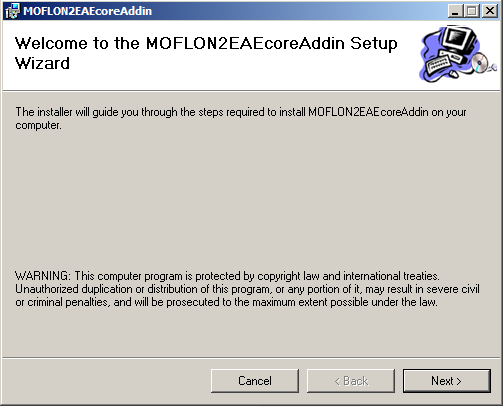
\includegraphics[width=0.3\textwidth]{pics/eaplugin_install.png}
	\caption{Install our plugin for EA.}
	\label{fig_eaPluginWizard}
\end{figure}
\end{enumerate}
\vspace{-1cm}

\section{Install Our Plugin for Eclipse}
\begin{enumerate}
\item[$\blacktriangleright$] Download and install Eclipse for Modeling
``Eclipse Modeling Tools (includes Incubating components)''
(Fig.~\ref{fig_downloadModelingPackage}) from:\\  
\url{http://www.eclipse.org/downloads/packages/}
\begin{figure}[!h]
	\centering
  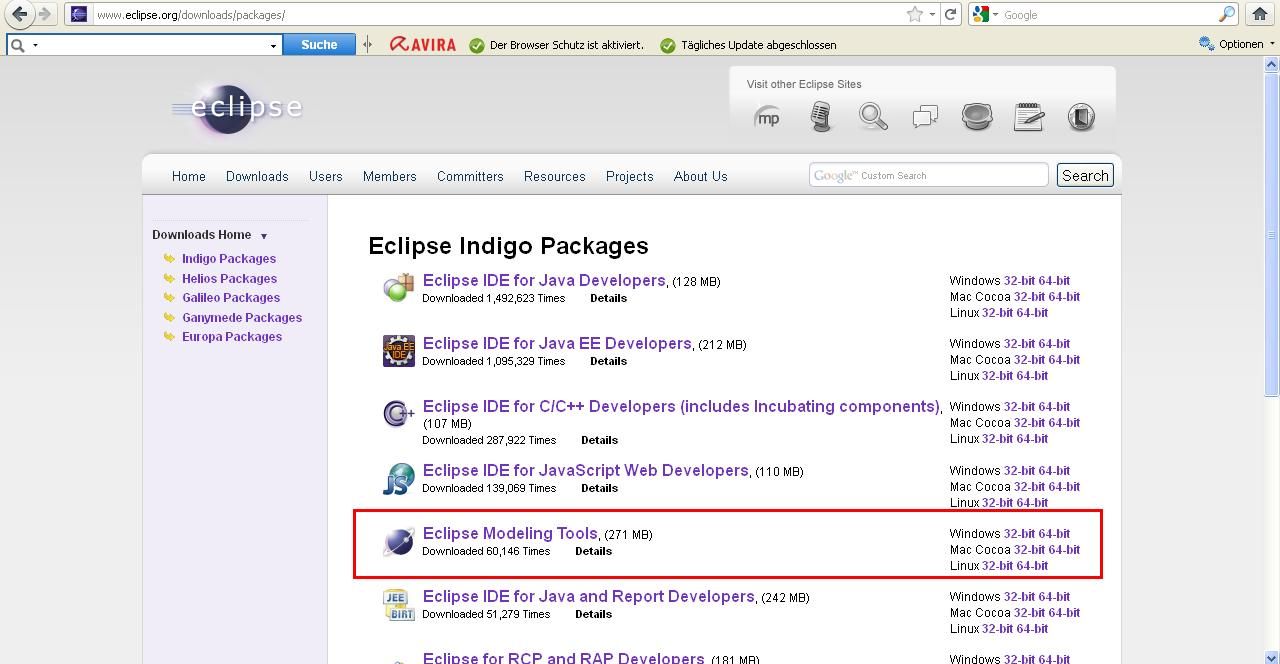
\includegraphics[width=0.7\textwidth]{pics/eclipse_modelingpackage.png}
	\caption{Download Eclipse Modeling Tools.}
	\label{fig_downloadModelingPackage}
\end{figure}
\vspace{-0.5cm}
\item[$\blacktriangleright$] Install our Eclipse Plugin from the following
update site\footnote{For a detailed tutorial on how to install Eclipse and
Eclipse Plugins please refer to
\url{http://www.vogella.de/articles/Eclipse/article.html}} 
\footnote{Please note: Calculating requirements and dependencies when installing
the plugin might take quite a while depending on your internet connection.}:
\url{http://www.moflon.org/fileadmin/download/moflon-ide/eclipse-plugin/update-site2}
\end{enumerate}

\section{Get a Simple Demo Running}

\begin{enumerate}
\item[$\blacktriangleright$] Go to ``Window/Open Perspective/Other\ldots'' and
choose Moflon (Fig.~\ref{fig_eclipse}).
\begin{figure}[!h]
	\centering
  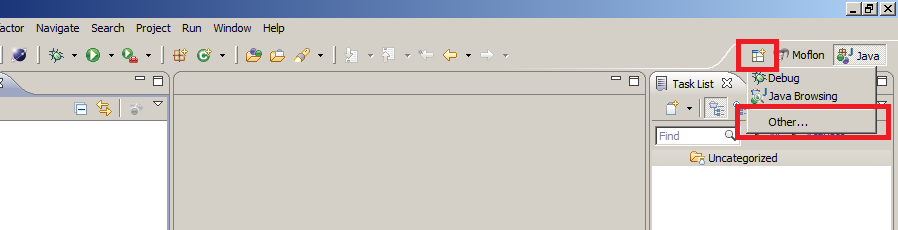
\includegraphics[width=0.7\textwidth]{pics/eclipse_firststart.png}
	\caption{Choose the Moflon Perspective.}
	\label{fig_eclipse}
\end{figure}

\item[$\blacktriangleright$] In the toolbar a new action set should have
appeared. Choose ``New Metamodel'' (Fig.~\ref{fig_eclipseNewMetamodel}).
The button with an ``L" shows you our logfile (important input for us if
something goes wrong!).
\begin{figure}[!h]
	\centering
  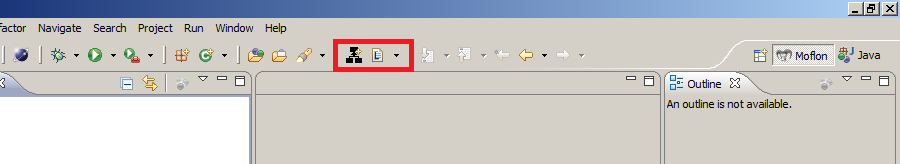
\includegraphics[width=0.8\textwidth]{pics/eclipse_metamodelButton.png}
	\caption{Eclipse New Metamodel}
	\label{fig_eclipseNewMetamodel}
\end{figure}

\item[$\blacktriangleright$] Enter ``Demo'' as the name of the new metamodel
project and confirm. 
An empty EA project file ``Demo.eap'' will be
created in a new project with a certain project structure
according to our conventions.

\newpage

\item[$\blacktriangleright$] Choose working sets as your top level element in
the package explorer (Fig.~\ref{fig_eclipseWorkingsets}).
We work a lot with working sets and use them to structure the workspace in
Eclipse.
\begin{figure}[!h]
	\centering
  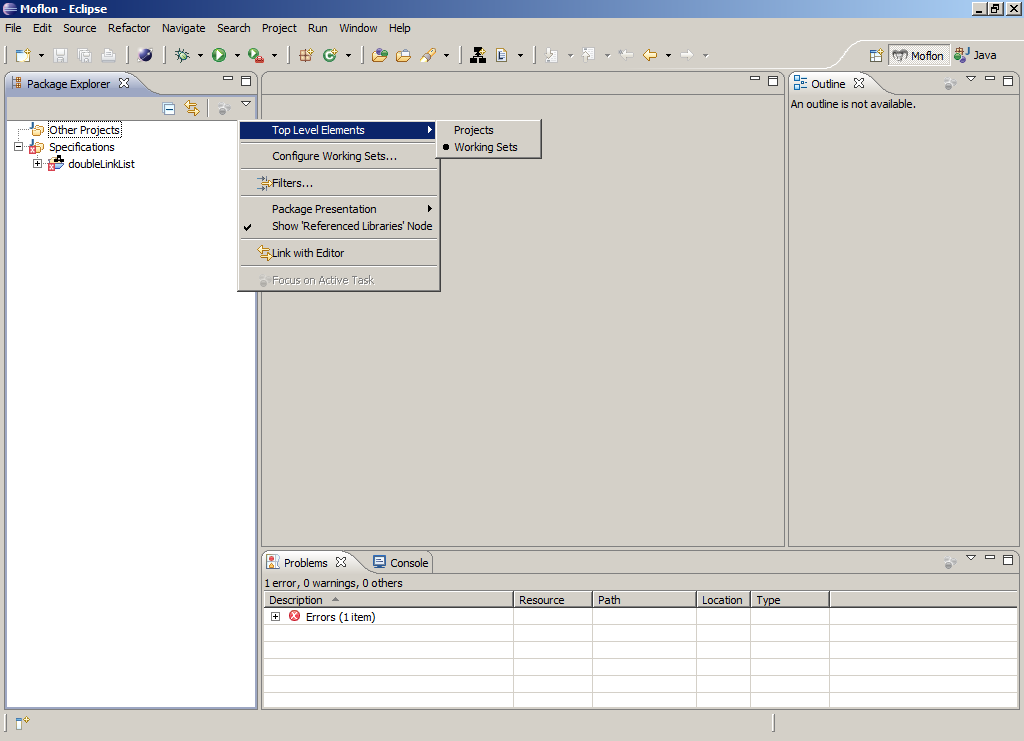
\includegraphics[width=0.6\textwidth]{pics/eclipse_workingsets.png}
	\caption{Choose Working Sets as Top Level Elements.}
	\label{fig_eclipseWorkingsets}
\end{figure}

\item[$\blacktriangleright$] Open the newly created project and replace the
``Demo.eap'' file with the Demo.eap that you will find in the
same folder as this tutorial. 
This EA file already contains our simple demo project.

\item[$\blacktriangleright$] Double click ``Demo.eap'' to start EA.
Please choose ``Ultimate" when starting EA for the first time.

\item[$\blacktriangleright$] In EA, choose ``Add-Ins/MOFLON::Ecore Addin/Export
all to Workspace'' (Fig.~\ref{fig_ea}).
\begin{figure}[!h]
	\centering
  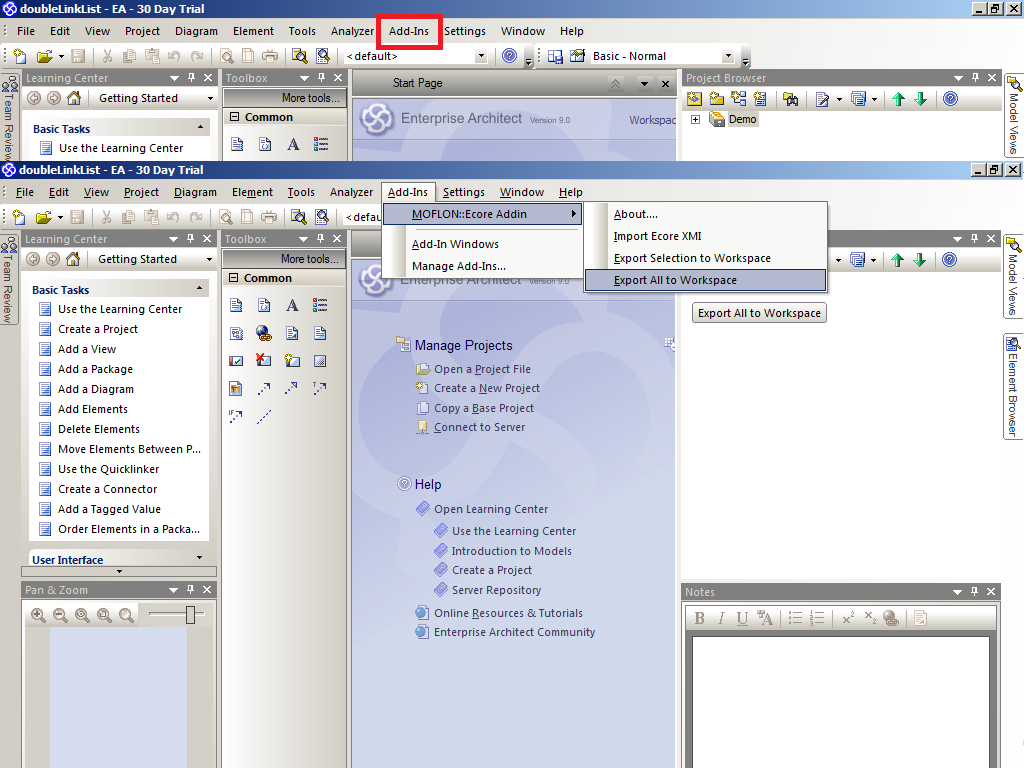
\includegraphics[width=0.65\textwidth]{pics/ea_firststart.png}
	\caption{Export from EA with our plugin.}
	\label{fig_ea}
\end{figure}

\newpage

\item[$\blacktriangleright$] Switch back to Eclipse, choose your Metamodel
project and press F5 to refresh.
The export from EA places all required files in a hidden folder in the
project, and refreshing triggers a build process that invokes our different
code generators automatically.
You should be able to monitor the progress in the lower right corner
(Fig.~\ref{fig_eclipsebuilding}).  
Pressing the symbol opens a monitor view that gives more details of the build
process. 
\begin{figure}[!h]
	\centering
  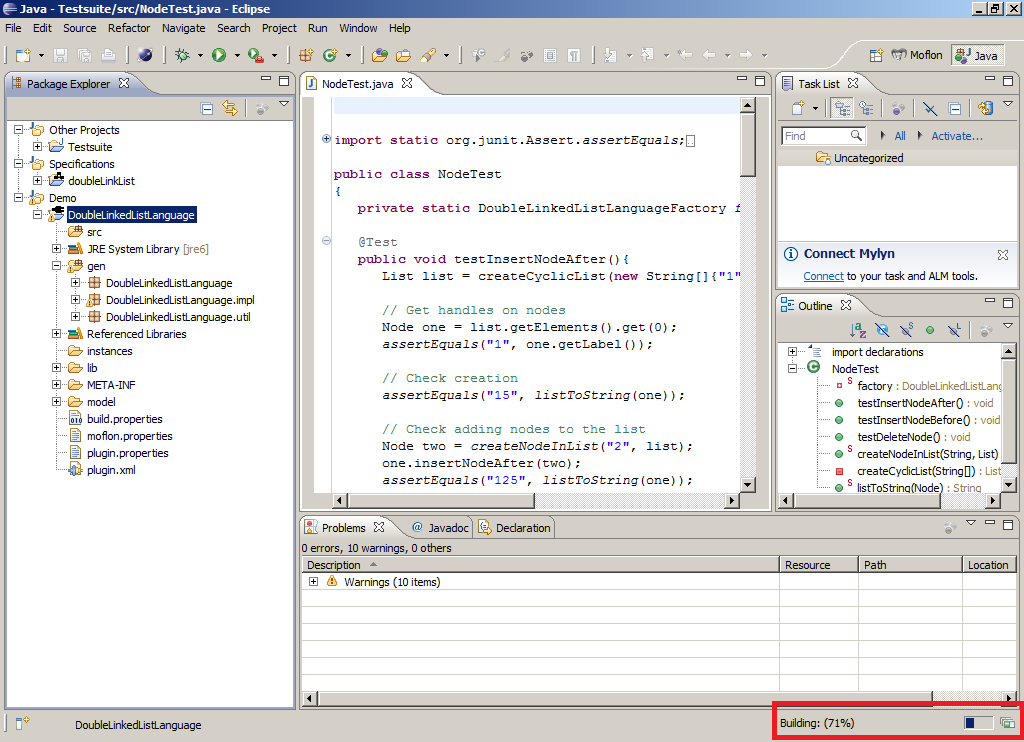
\includegraphics[width=0.6\textwidth]{pics/eclipse_building.png}
	\caption{Automatically building the workspace after a refresh.}
	\label{fig_eclipsebuilding}
\end{figure}
\end{enumerate}

\section{Validate Your Installation with JUnit}

\begin{enumerate}
\item[$\blacktriangleright$] Go to ``File/Import/General/Existing Projects
into Workspace'' (Fig.~\ref{fig_eclipseTestsuiteImport}) and choose the
Testsuite project that is also in the same folder as this tutorial. 
\begin{figure}[!h]
	\centering
  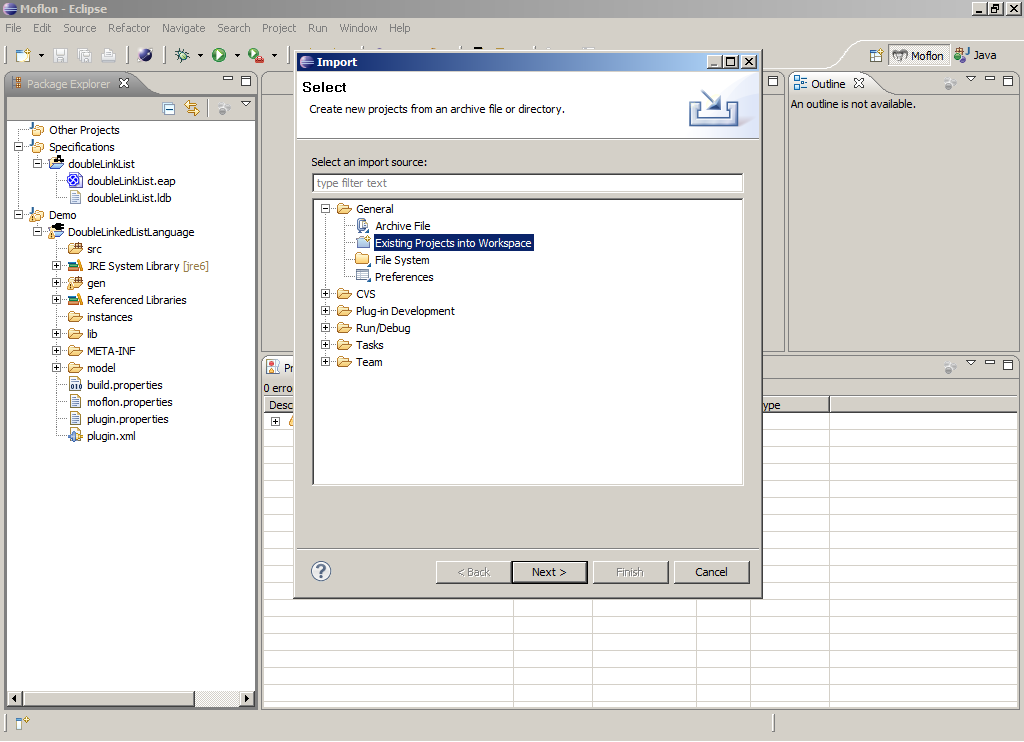
\includegraphics[width=0.6\textwidth]{pics/eclipse_testsuitimport.png}
	\caption{Import our Testsuite as an existing project.}
	\label{fig_eclipseTestsuiteImport}
\end{figure}

\newpage 

\item[] At this point, your workspace should resemble
Fig.~\ref{fig_eclipsepackageexplorer}.
\begin{figure}[!h]
	\centering
  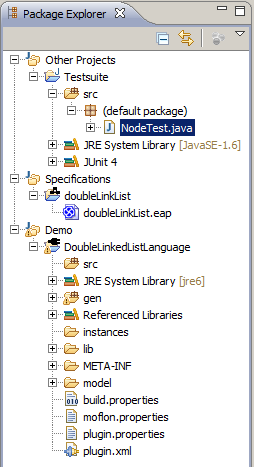
\includegraphics[width=0.2\textwidth]{pics/eclipse_packageexplorer.png}
	\caption{Workspace in Eclipse.}
	\label{fig_eclipsepackageexplorer}
\end{figure}

\item[$\blacktriangleright$] Right-click on the Testsuite project and select
``Run as/JUnit Test''.
Congratulations!  If you see a green bar  (Fig.~\ref{fig_eclipsetestsuiterun}),
then everything has been set-up correctly and you are now ready to start
metamodelling!
\begin{figure}[!h]
	\centering
  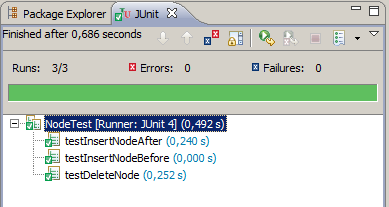
\includegraphics[width=0.2\textwidth]{pics/eclipse_testsuiterun.png}
	\caption{All's well that ends well\ldots}
	\label{fig_eclipsetestsuiterun}
\end{figure}
\end{enumerate}



\section{Project Structure and Setup}
Now that everything is installed and setup properly, let's take a closer look at
the different workspaces and workflow.  Before we continue, please make
a few slight adjustments to EA so you can easily compare your current workspace 
to our screenshots:
\begin{itemize}
  \item[$\blacktriangleright$] Select ``Tools/Options/Standard Colors'' in EA,
  and set your colours to reflect Fig.~\ref{fig_standardColoursEA}.
  \item[$\blacktriangleright$] In the same dialogue, select
  ``Diagram/Appearance'' and reflect the settings in
  Fig.~\ref{fig_standardAppearanceEA}.
  \item[$\blacktriangleright$] Last but not least, and still in the same
  dialogue, select ``Source Code Engineering'' and be sure to choose ``Ecore''
  as the default language for code generation (Fig.~\ref{fig_standardSCEEA}).
\end{itemize}
\newpage
%\usepackage{graphics} is needed for \includegraphics
\begin{figure}[!h]
\centering
\begin{minipage}[b]{0.3\textheight}
  \centering
  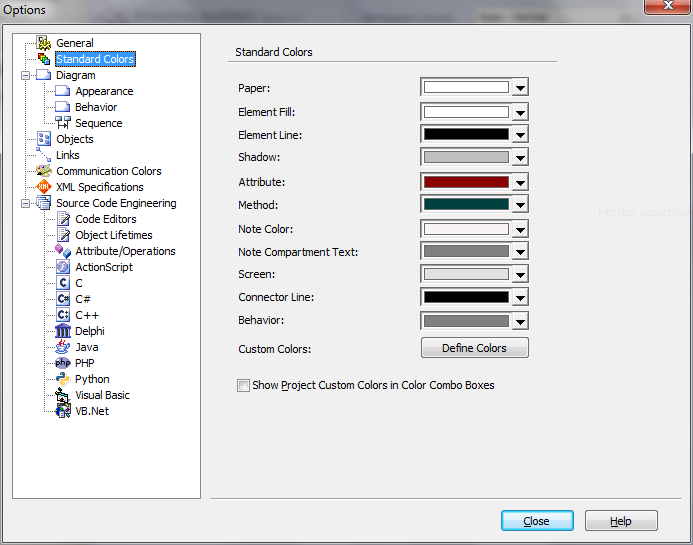
\includegraphics[width=\textwidth]{pics/standardColours}
  \caption{Our choice of standard colours for diagrams in EA.}
  \label{fig_standardColoursEA}
\end{minipage}
\\
\vspace{0.5cm}
\begin{minipage}[b]{0.3\textheight}
  \centering
  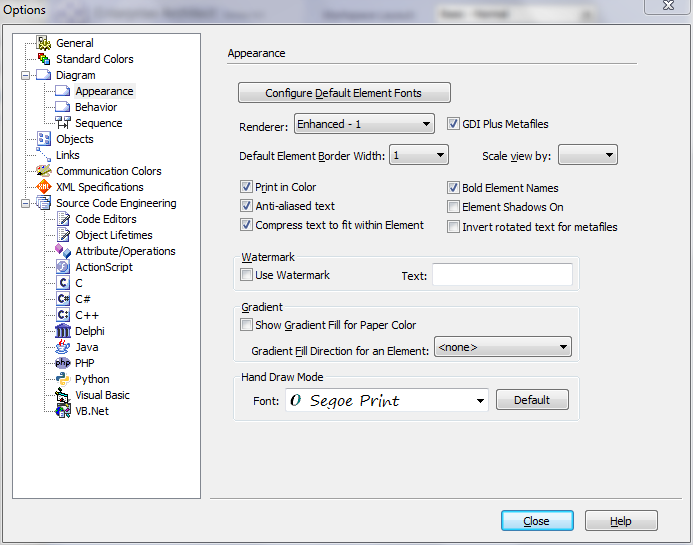
\includegraphics[width=\textwidth]{pics/standardAppearance}
  \caption{Our choice of the standard appearance for model elements in EA.}
  \label{fig_standardAppearanceEA}
\end{minipage}
\\
\vspace{0.5cm}
\begin{minipage}[b]{0.3\textheight}
  \centering
  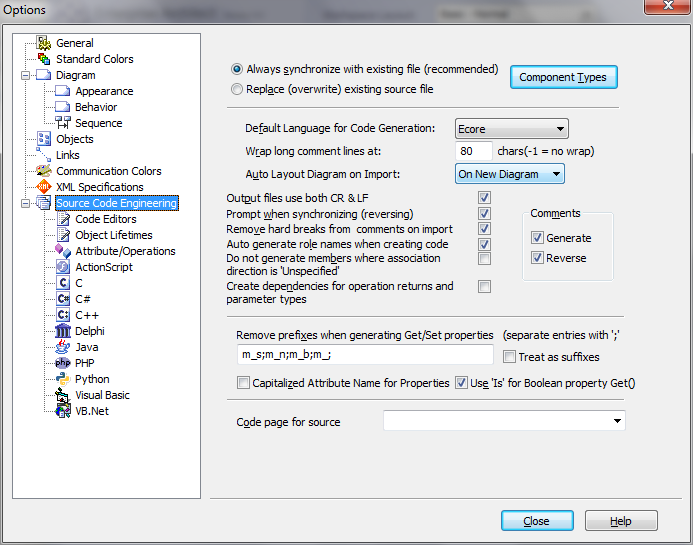
\includegraphics[width=\textwidth]{pics/standardCodeEngineering}
  \caption{Make sure you set the standard language to Ecore.}
  \label{fig_standardSCEEA}
\end{minipage}
\end{figure}

In your EA ``workspace'', actually referred to as an \emph{EA
project}\footnote{Words are set in italics when they represent concepts that are
introduced or defined  in the corresponding paragraph for the first time.}, take
a careful  look at the project structure:  The root node
\texttt{Demo}\footnote{Words set  in a \texttt{mono-space font} refer to things
that you should find in a tool,  dialogue, figure or code.} is called a
\emph{model} in EA lingo and is used as a  container to group a set of related
\emph{packages}. In our case, \texttt{Demo}  consists of a single package
\texttt{DoubleLinkedListLanguage}.  An EA project can however consist of
numerous models that in turn group  numerous packages.


Now switch to your \emph{Eclipse workspace} and note the two nodes named
\texttt{Spe\-ci\-fi\-ca\-tions} and \texttt{Demo}.  These nodes, used to group
related \emph{Eclipse projects} in an Eclipse workspace, are called
\emph{working sets}. The working set \texttt{Spe\-ci\-fi\-ca\-tions} contains
all \emph{metamodel projects} in a  workspace.
 A metamodel project contains a single EAP (EA project) file and is
used to communicate with EA and initiate codegeneration by simply pressing F5
or choosing ``refresh'' from the context menu.  In our case,
\texttt{Specifications} should contain a single metamodel project \texttt{Demo}
containing our EA project file  \texttt{Demo.eap}.

\begin{figure}[!h]
	\centering
  \includegraphics[width=0.8\textwidth]{pics/bothexplorers}
	\caption{From EA to Eclipse}
	\label{fig_fromEAtoEclipse}
\end{figure}

Figure~\ref{fig_fromEAtoEclipse} depicts how the Eclipse working set
\texttt{Demo} and its contents were generated from the EA model \texttt{Demo}.
Every model in EA is mapped to a working set in Eclipse with the same name. 
From every packages in the EA model, an Eclipse project is generated, also with
the same name.  These projects, however, are of a different
\emph{nature} than for example metamodel projects or normal Java projects, and
are called \emph{repository projects}.  A nature is Eclipse lingo for ``project
type'' and is visually indicated by a corresponding nature icon on the project
folder.  Our  metamodel projects sport a spanking little class diagram symbol. 
Repository projects are generated automatically  with a certain project
structure according to our conventions.  The  \texttt{model} subfolder is
probably most important, and contains an  \emph{Ecore model}.  Ecore is a
metamodelling language that provides building  blocks like \emph{classes} and
\emph{references} for defining the  static structure (concepts and relations
between concepts) of a system.  The  export function of our EA plugin generates
a valid Ecore model from the  corresponding EA model and persists it as an XML
file in the \texttt{model}  subfolder.  In our concrete example, this is the
\texttt{DoubleLinkedListLanguage.ecore} file.  Go ahead and double-click it to
open the file in a simple tree-view editor in Eclipse.  If you are really
interested in the nitty-gritty details or have a masochistic hang, right-click
the file and select ``Open With/Text Editor''. 

This Ecore model is used to drive a codegenerator that maps the model to Java
interfaces and classes.  The generated Java code that represents the model is
often referred to as a \emph{repository} and this is the reason why we refer to
such projects as repository projects.  A repository can be viewed as an
\emph{adapter} that enables building and manipulating concrete instances of a
specific model via a programming language like Java.  This is why we
indicate repository projects using a cute adapter/plug symbol on the project
folder.

Figure~\ref{fig_fromEAtoEclipse} depicts how the class \texttt{Node} in the EA
model is mapped to the Java interface \texttt{Node}.  Double-click
\texttt{Node.java} and take a look at the methods declared in the interface.
These correspond directly to the methods declared in the modelled \texttt{Node}
class.  Indicated by the source folders \texttt{src} and \texttt{gen}, we
advocate a clean separation of hand-written (this should go in \texttt{src}) and
generated code (lands automatically in \texttt{gen}).  As we shall see later in
the tutorial, hand-written code can also be integrated directly in generated
classes and, if marked appropriately, merged nicely by the codegenerator. 
This is sometimes more elegant for small helper functions but can quickly get
problematic especially in combination with source code management systems.

If you take a careful look at the code structure in \texttt{gen},
you'll find a \texttt{Foo\-Impl.java} for every \texttt{Foo.java}. Indeed, the 
subpackage \texttt{impl} contains Java classes that implement the interfaces in
the parent package.  Although this might strike you as unnecessary (why not
merge interface and implementation for simple classes?), this consequent
separation in interfaces and implementation allows for a clean and relatively
simple mapping of Ecore to Java, even in tricky cases like multiple inheritance
(allowed and very common in Ecore models).  A further package \texttt{util}
contains some auxiliary classes like a factory for creating instances of the
model.  If this is your first time of seeing generated code, you might be
shocked at the sheer amount of classes and code generated from our relatively
simple EA model.  You might be thinking: ``hey - if I did this by hand I
wouldn't need half of all this stuff!''.  Well you're right and you're wrong --
the point is that an automatic mapping to Java via a codegenerator scales quite
well.  This means for simple, trivial examples (like our double linked list), it
might be possible to come up with a leaner and simpler Java representation.  For
complex, large models with lots of mean pitfalls, however, this becomes a
daunting task.  The codegenerator provides you with years and years of
experience of professional programmers who have thought up clever ways
of handling multiple inheritance, an efficient event mechanism, reflection,
consistency between bidirectionally linked objects and much more.

A point to note here is that the mapping to Java is obviously not unique. 
Indeed there exist different standards of how to map a modelling language to a
general purpose programming language like Java.  We use a mapping defined and
implemented by the Eclipse Modelling Framework (EMF) which tends to favour
efficiency and simplicity.

Although getting the \emph{details} of mapping the static structure of our
models to Java might be extremely difficult, it seems for the most part pretty
straight  forward.  A fantastic productivity boost in any case but (yawn) not
exactly exciting.

Have you noticed the methods of the \texttt{Node} class in our EA model? 
Now hold on tight -- each method can be \emph{modelled} completely in EA and the
corresponding implementation in Java is generated automatically and placed in
\texttt{NodeImpl}.  Just in case you didn't get it: 
The behavioural or dynamic aspects of a system can be completely modelled in an
abstract, platform (programming language) independent fashion using a blend of
activity  diagrams and a ``graph pattern'' language called Story Driven
Modelling (SDM).  In our EA project, these ``Stories'', ``Story Models'' or
simply ``SDMs'' are  placed in SDM Containers named according to the method they
implement.  E.g.  \texttt{$\ll$ SDM Container$\gg$ insertNodeAfter SDM} for the
method  \texttt{insertNodeAfter(Node)} as depicted in
Fig.~\ref{fig_fromEAtoEclipse}.  We'll spend the rest of the tutorial
understanding why SDMs are so  {\huge crazily} cool!

\clearpage

To recap all we've discussed, let's consider the complete workflow as depicted
in Figure~\ref{fig_Overview}. We started with a concise model in EA, simple and
independent of any platform specific details (1).  Our EA model consists not
only of static aspects modelled as a class diagram (2), but also of dynamic
aspects modelled using SDM (3).  After exporting the model and codegeneration
(4), we basically switch from \emph{modelling}, to \emph{programming} in a
specific general purpose programming language (Java).  On this lower \emph{level
of abstraction}, we can flesh out the generated repository (5) if necessary, and 
mix as appropriate with hand-written code and libraries.  Our abstract specification of 
behaviour (methods) in SDM is translated to a series of method calls that form
the body of the corresponding Java method (6).
\begin{figure}[!h]
	\centering
  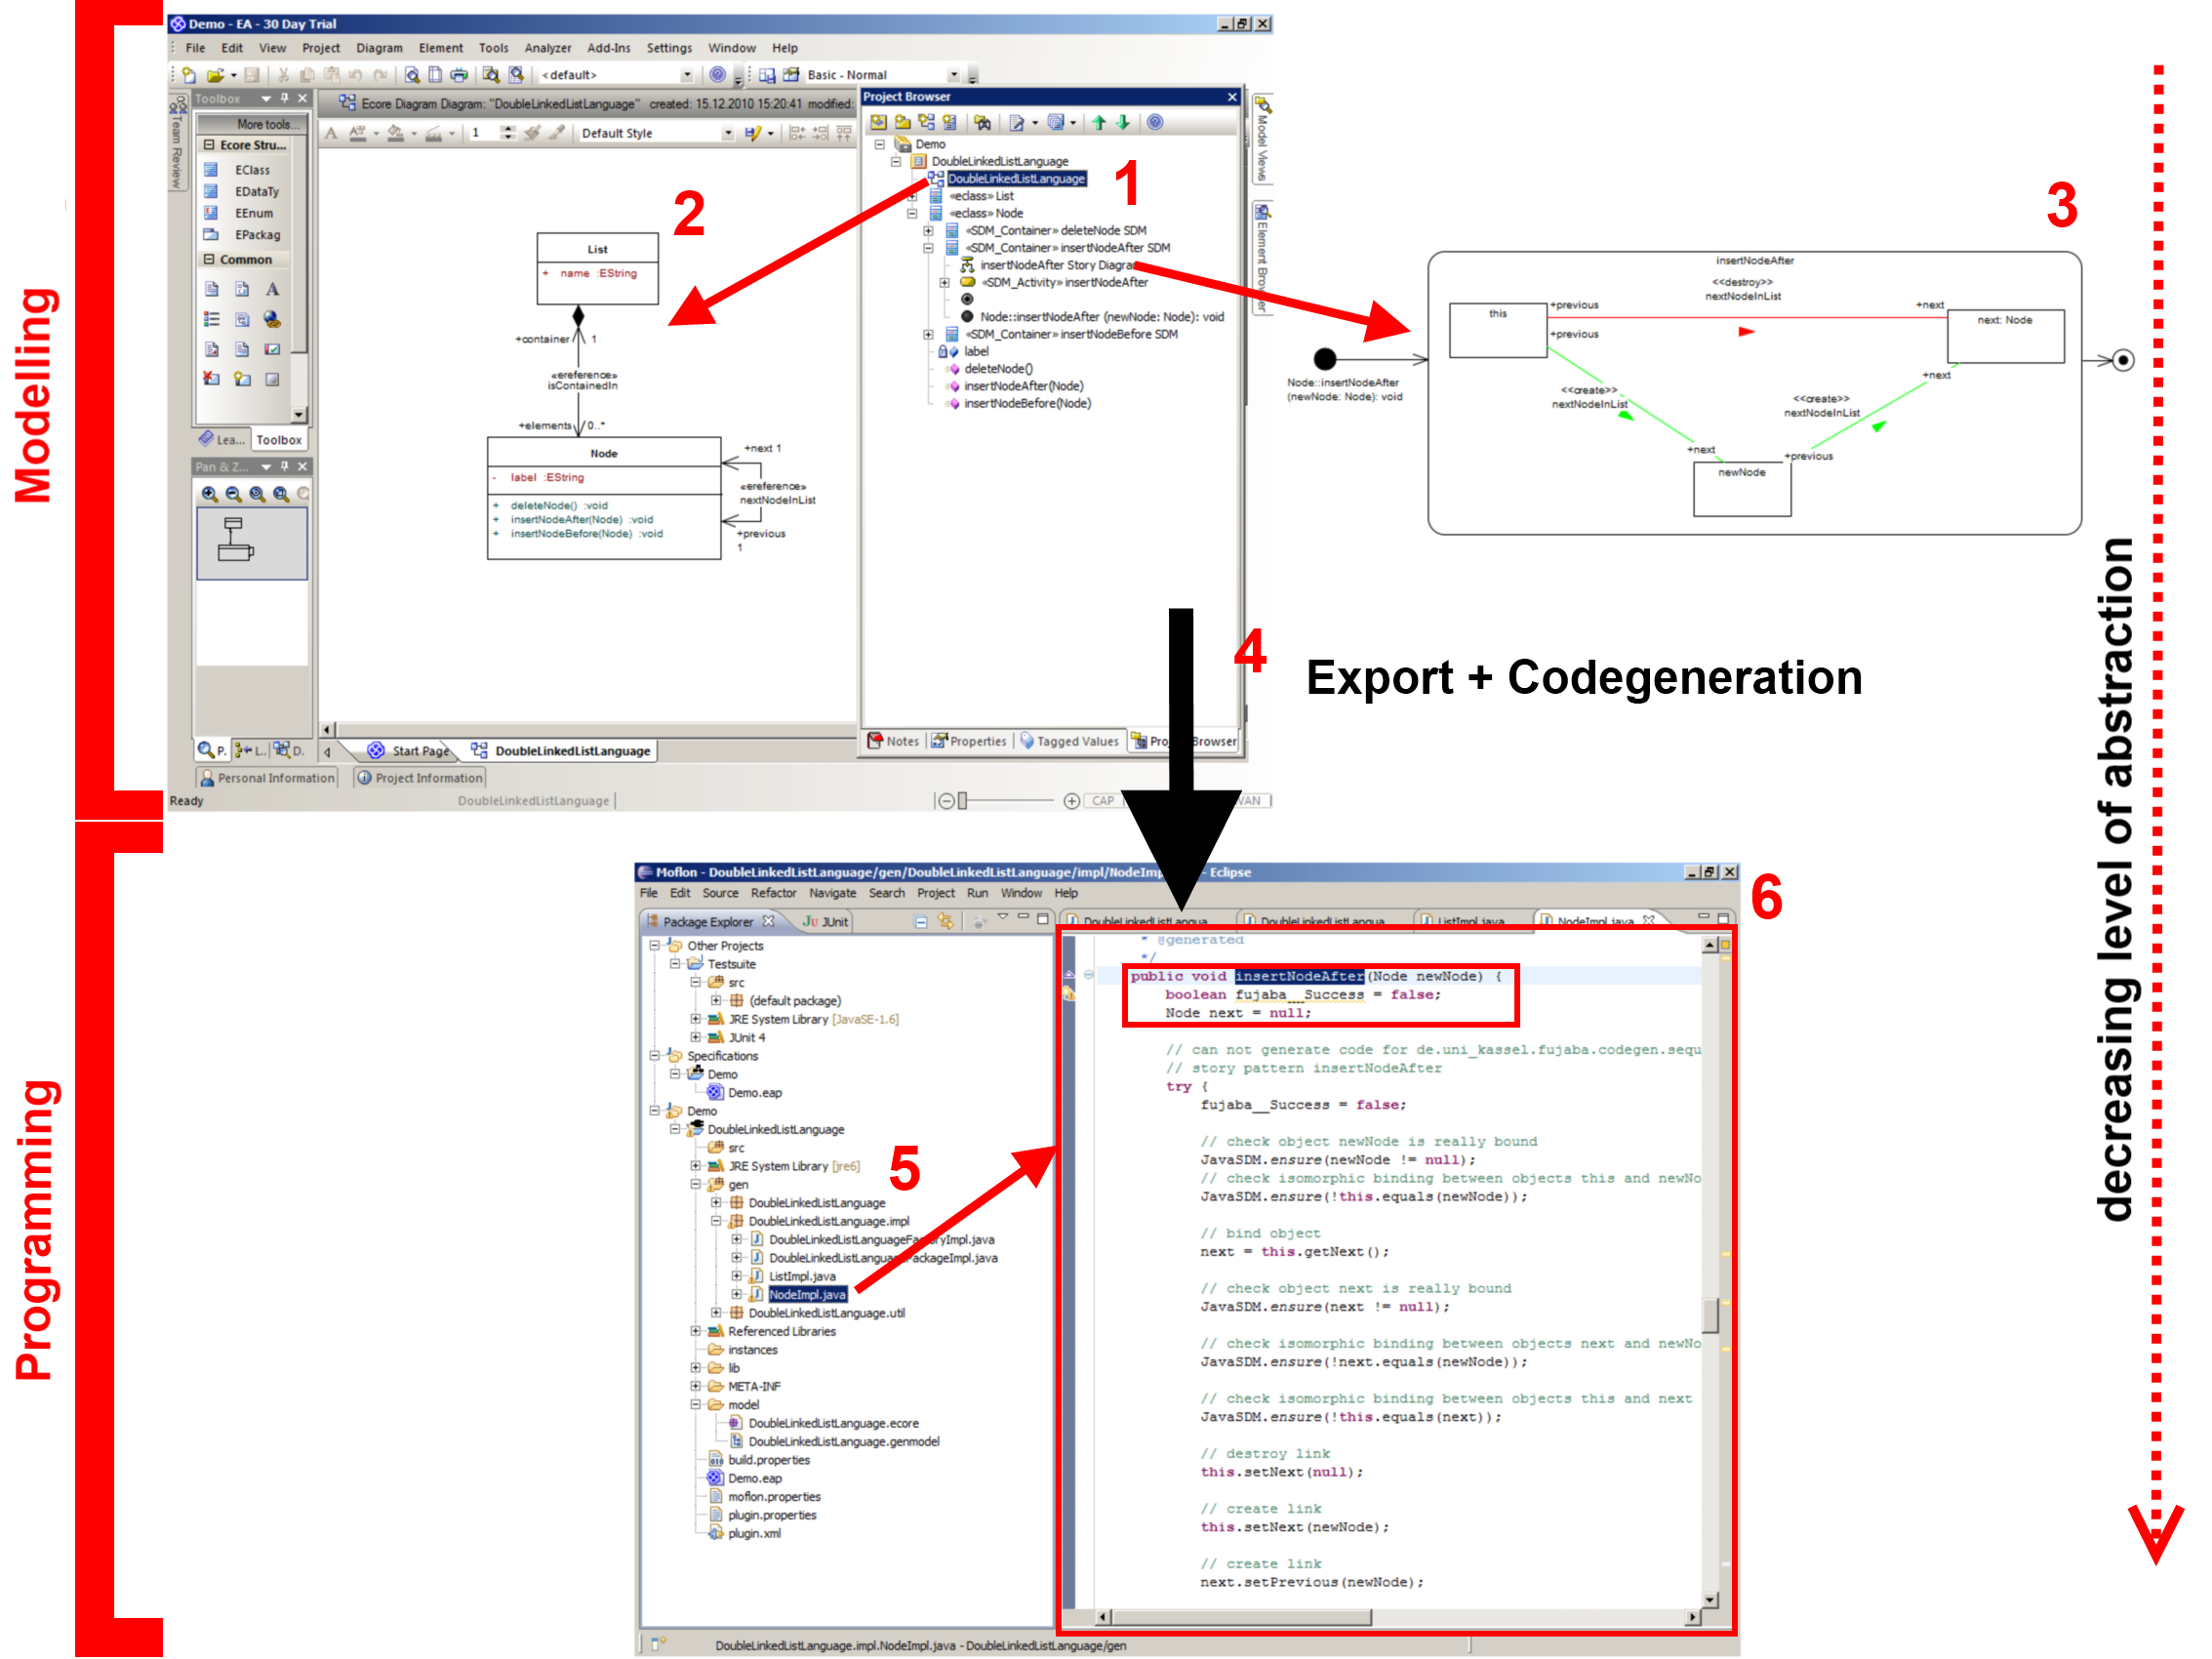
\includegraphics[width=1\textwidth]{pics/tafelbild}
	\caption{Overview}
	\label{fig_Overview}
\end{figure}


If you feel a bit lost at the moment please be patient, this first chapter has
been a lot about installation and tool support and only aims at giving a very
brief glimpse at the big picture of what is actually going on.    

In the following chapter, we shall go step-by-step through a hands-on example
and cover the core features of Ecore (static structure) and SDM (behaviour). 
We shall also give clear and simple definitions for the most important
metamodelling and graph transformation concepts, always referring to the
concrete example and providing lots of references for further reading.
\chapter{Modelling a Memory Box}
\label{chap:membox}

 The toughest part of learning a new language  is often building up a sufficient
vocabulary.  This is usually accomplished by repeating a long list of words
again and again till they stick.  A memory box is a simple but ingenious little
contraption to support this tedious process of memorisation.  As depicted in
Fig.~\ref{fig:membox_illustration}, it consists of a series of compartments or
partitions usually of increasing size.  The content to be memorised is written
on a series of cards  which are initially placed in the first partition.  All
cards in the first  partition should be repeated everyday and cards that have
been successfully  memorised are placed in the next partition.  Cards in all
other partitions are  only repeated when the corresponding partition is full and
cards that are  answered correctly are moved one partition forward in the box. 
Challenging  cards that have been forgotten are treated as brand new cards and
are always  placed right back into the first partition regardless of how far in
the box they  had progressed.  These ``rules'' are depicted by the green and red
arrows in  Fig.~\ref{fig:membox_illustration}. The basic idea is to repeat
difficult cards as often as necessary  and not to waste time on easy cards which
are only repeated now and then to keep them in memory.  The  increasing size of
the partitions represents how words are easily placed in our limited short term
memory and slowly move in our theoretically unlimited long term memory if
practised often enough.

%\usepackage{graphics} is needed for \includegraphics
\begin{figure}[htp]
\begin{center}
  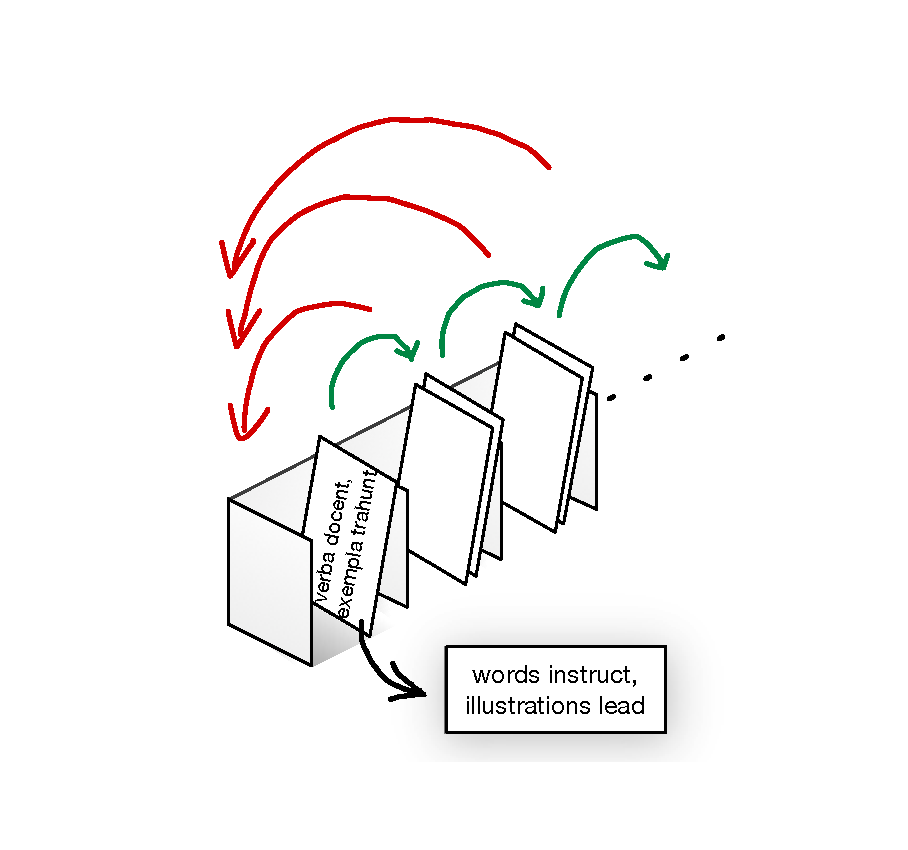
\includegraphics[width=0.4\textwidth]{pics/membox_illustration}
  \caption[]{Possible \emph{Concrete Syntax} of our Memory Box.}
  \label{fig:membox_illustration}
\end{center}
\end{figure}

A memory box is an interesting system, because it consists clearly of a static
structure (the box, partitions and their sizes, cards with their sides and
corresponding content) and a set of rules that describe the dynamic aspects 
(behaviour) of the system.  In the rest of the tutorial we shall build a
complete memory box from scratch in a model-driven fashion and use it to
introduce fundamental concepts in metamodelling and MDSD in general.  

\section*{A Language Definition Problem?}

Like in any area of study, metamodelling has its fair share of buzz words used
by experts to communicate concisely.  Although some concepts might seem quite
abstract for a beginner, a well defined vocabulary is important so we know
exactly what we are talking about.   

The first step is understanding that metamodelling equates to language
definition.  This means that the task of building a system like our memory box
can be viewed as defining a suitable language that can be used to describe the
system.  This language oriented approach has a lot of advantages including a
natural support for product lines (individual products are valid members of the
language) and a clear separation between platform independent and platform
specific details.      

So what constitutes a language?  The first question is obviously  how the
building blocks of your language actually ``look'' like.  Is your language to be
textual?  Visual?  This is referred to as the \emph{Concrete Syntax} of a
language and is basically an interface to end users who use the language.  
\marginpar{\emph{Concrete Syntax}}
In the case of our memory box, Fig.~\ref{fig:membox_illustration} can be viewed
as a possible concrete syntax.  As we are however building a memory box as a
software system, our actual concrete syntax  will probably be composed of GUI
elements like buttons, drop-down menus and text fields.   

Irrespective of how a language looks like, members of the language must adhere
to the same set of ``rules''.  
\marginpar{\emph{Grammar}}
For a natural language like English, this set of rules is usually called a
\emph{grammar}.  
In metamodelling, however, everything is represented as a graph of some kind
and, although the concept of a  \emph{graph grammar} is also quite well-spread
and understood, metamodellers  more often use a \emph{type graph} that defines
what types and relations  constitute a language. 
\marginpar{\emph{Graph Grammar}}
\marginpar{\emph{Type Graph}}
A graph that is a member of your language must \emph{conform to} the
corresponding type graph for the language.  To be more precise, it must be
possible to type the graph according to the type graph, i.e., the types and
relations used in the graph must exist in the type graph and not contradict the
structure defined there.  
\marginpar{\emph{Abstract Syntax}}
This way of defining membership to a language has many parallels to the
class-object relationship in the Object Oriented paradigm and should seem very
familiar for any programmer used to OO.  This type graph is referred to as the
\emph{Abstract Syntax} of a language. 

Very often, one might want to further constrain a language, beyond simple typing
rules.  
\marginpar{\emph{Static Semantics}}  
This can be accomplished with a further set of rules or constraints that
members of the language must fulfil in addition to being conform to the type
graph.
These further constraints are referred to as the \emph{Static Semantics}
of a language.    

With these few basic concepts, we can now introduce a further and central
concept in metamodelling, the \emph{metamodel} (basically a simple class
diagram). 
\marginpar{\emph{Metamodel}}
A metamodel defines not only the abstract syntax of a language but also some
basic constraints (a part of the static semantics).  
Thinking back to our memory box, we could define the types and relations we want
to allow, e.g.,  a box with partitions, cards, the box contains partitions that
contain cards. 
Multiplicities are an example for constraints that are no longer part of the
abstract syntax and belong to static semantics, but can nonetheless be expressed
in a metamodel.
For example, that a card can only be in one partition, or that a partition has
only one next partition or none.
\marginpar{\emph{Constraint Language}}  
More complex constraints that cannot be expressed in a metamodel are usually
specified using an extra \emph{constraint language} such as OCL (the Object
Constraint Language).
This goes beyond this tutorial however and we'll stick to metamodels without
using an extra constraint language.              

A short recap:  we have learnt that metamodelling starts with defining a
suitable language.  
For the moment, we know that a language comprises a concrete
syntax (how does the language look like),  an abstract syntax (types and
relations of the underlying graph structure), and static semantics (further
constraints that members of the language must fulfil).
\marginpar{\emph{Model}}
Metamodels are used to define the abstract syntax and a part of the static
semantics of a language, while \emph{models} are graphs that conform to some
metamodel (can be typed  according to the abstract syntax and adhere to the
static semantics). 

This tutorial is meant to be be hands-on so enough theory!  Lets
define, step-by-step, a metamodel for our memory box using our tool eMoflon.  
 
\section*{Abstract Syntax and Static Semantics with Ecore}

Switch to EA, choose \texttt{Demo} and click on the button \texttt{Add a
Package} as depicted in Fig.~\ref{fig:new_package}.   

\begin{figure}[htbp]
	\centering
  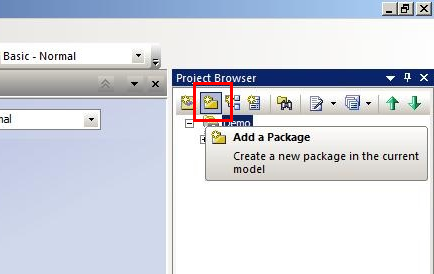
\includegraphics[width=0.5\textwidth]{pics/memBox01.png}
	\caption{Add a new package to \texttt{Demo}.}
	\label{fig:new_package}
\end{figure} 

In the dialogue that pops up (Fig.~\ref{fig:new_package_name}), choose
\texttt{Class View}, enter \texttt{Memory\-Box\-Language} as the name of the new
package and click \texttt{OK}. 

\begin{figure}[htbp]
	\centering
  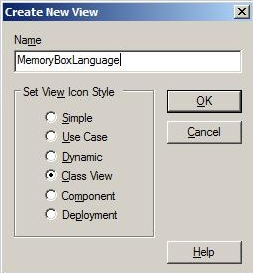
\includegraphics[width=0.3\textwidth]{pics/memBox02.png}
	\caption{Enter the name of the new package.}
	\label{fig:new_package_name}
\end{figure}

In your EA workspace the \texttt{Project Browser} should now look like
Fig.~\ref{fig:new_package_completed}.

\begin{figure}[htbp]
	\centering
  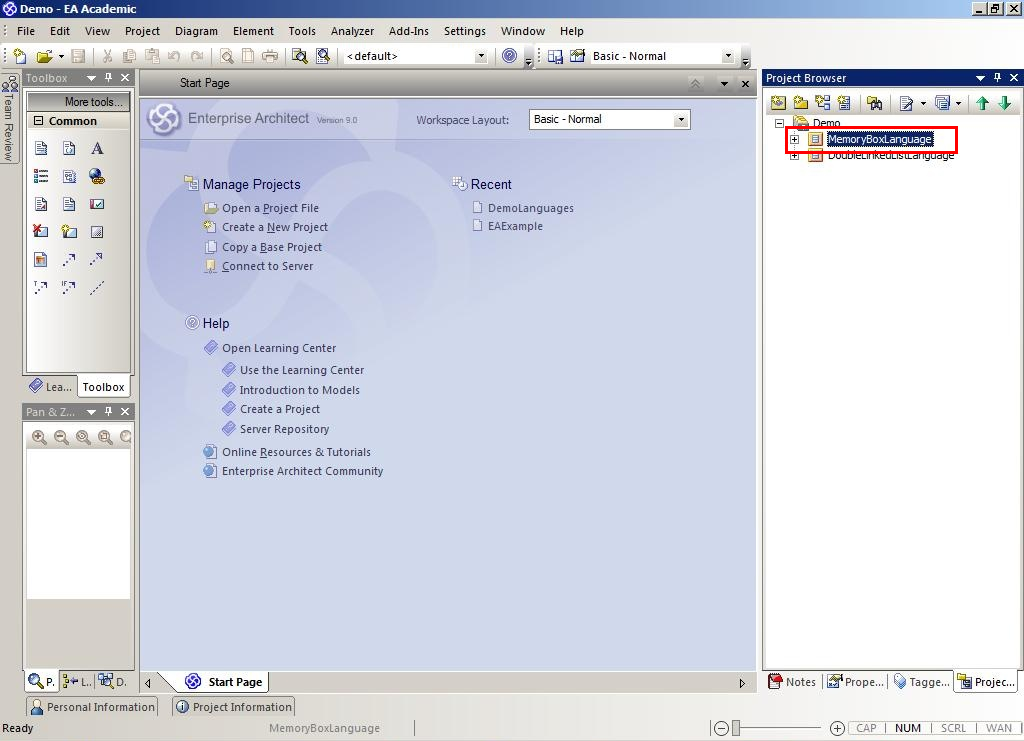
\includegraphics[width=0.5\textwidth]{pics/memBox03.png}
	\caption{State after creating the new package.}
	\label{fig:new_package_completed}
\end{figure}

\clearpage 

Now click the button \texttt{New Diagram} (Fig.~\ref{fig:diagram}).

\begin{figure}[htbp]
	\centering
  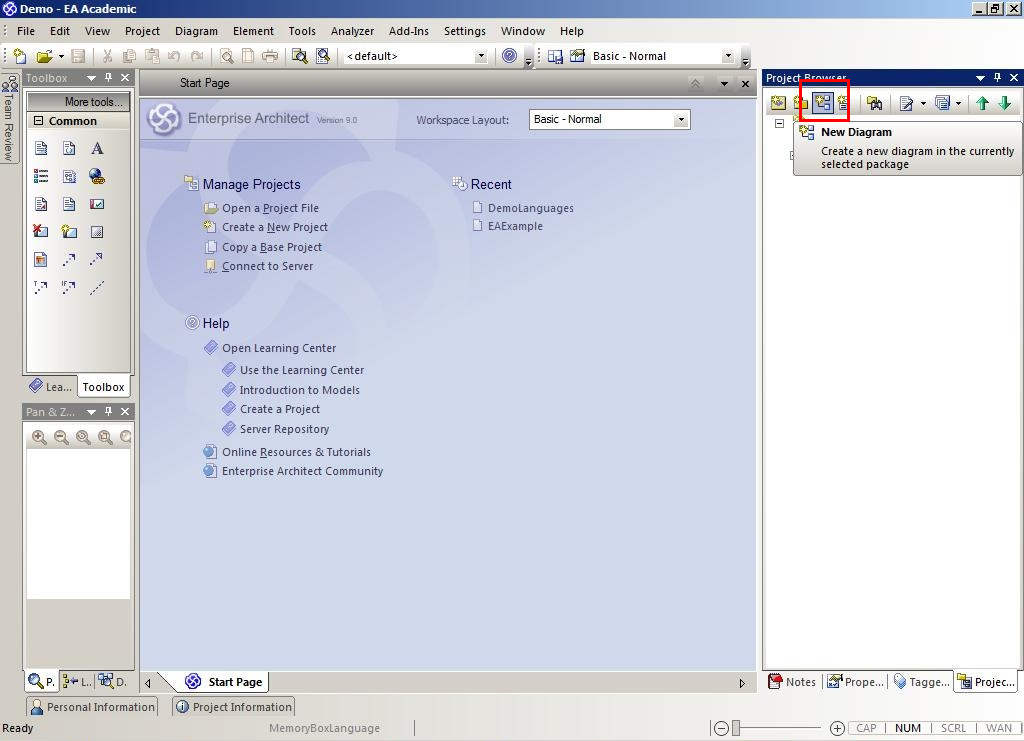
\includegraphics[width=0.7\textwidth]{pics/memBox04.png}
	\caption{Add a diagram.}
	\label{fig:diagram}
\end{figure}

In the dialog that pops up (Fig.~\ref{fig:diagram_type}), choose \texttt{Ecore
Diagram} and  \texttt{OK}. 


\begin{figure}[htbp]
	\centering
  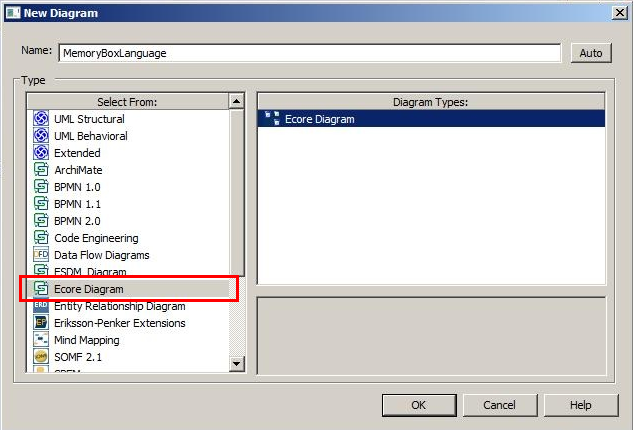
\includegraphics[width=0.8\textwidth]{pics/memBox05.png}
	\caption{Choose type of diagram.}
	\label{fig:diagram_type}
\end{figure}

In analogy to the ``everything is an object''
principle in the OO paradigm, in metamodelling, everything is a model.
\marginpar{\emph{Unification}}
This principle is called \emph{Unification} and has a lot of advantages.
If everything is a model, a metamodel that defines (at least a part of) a
language must be a model itself.
\marginpar{\emph{Meta-metamodel}}
\marginpar{\emph{Meta-Language}}
\marginpar{\emph{Modelling Language}}
This means that it conforms to some \emph{meta-metamodel} which defines a
\emph{(meta)modelling language} or \emph{meta-language}.
For metamodelling with eMoflon, we support \emph{Ecore} as a modelling language
and it defines types like \texttt{EClass} and \texttt{EReference}, which we will
be using to specify  our metamodels.
Other modelling languages include MOF, UML and Kermeta. 

\clearpage

After creating the new diagram, your  \texttt{Project Browser} should now
resemble Fig.~\ref{fig:diagram_completed}.  Double-click the newly
created diagram to ensure that it is open.

\begin{figure}[htbp]
	\centering
  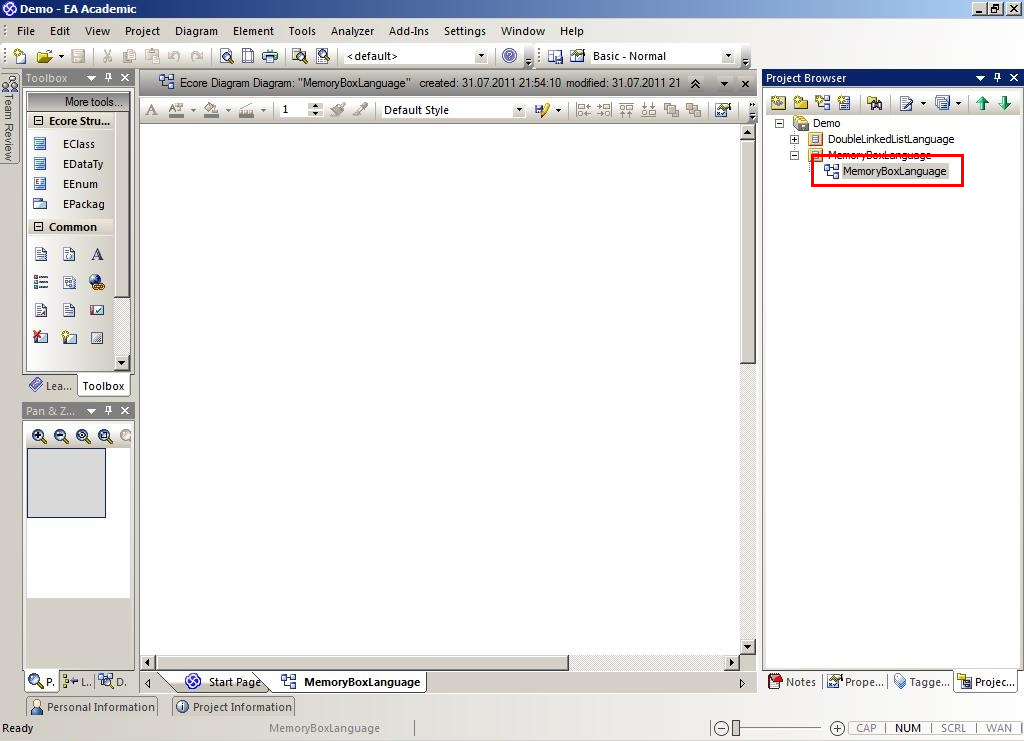
\includegraphics[width=0.7\textwidth]{pics/memBox06.png}
	\caption{State after creating diagram.}
	\label{fig:diagram_completed}
\end{figure}

To the left of the workbench in EA, a \emph{Toolbox} should have appeared
containing the types available in Ecore for metamodelling
(Fig.~\ref{fig:eclass}).  Click on \texttt{EClass} and click in the open
diagram (the main window in EA).

\begin{figure}[htbp]
	\centering
  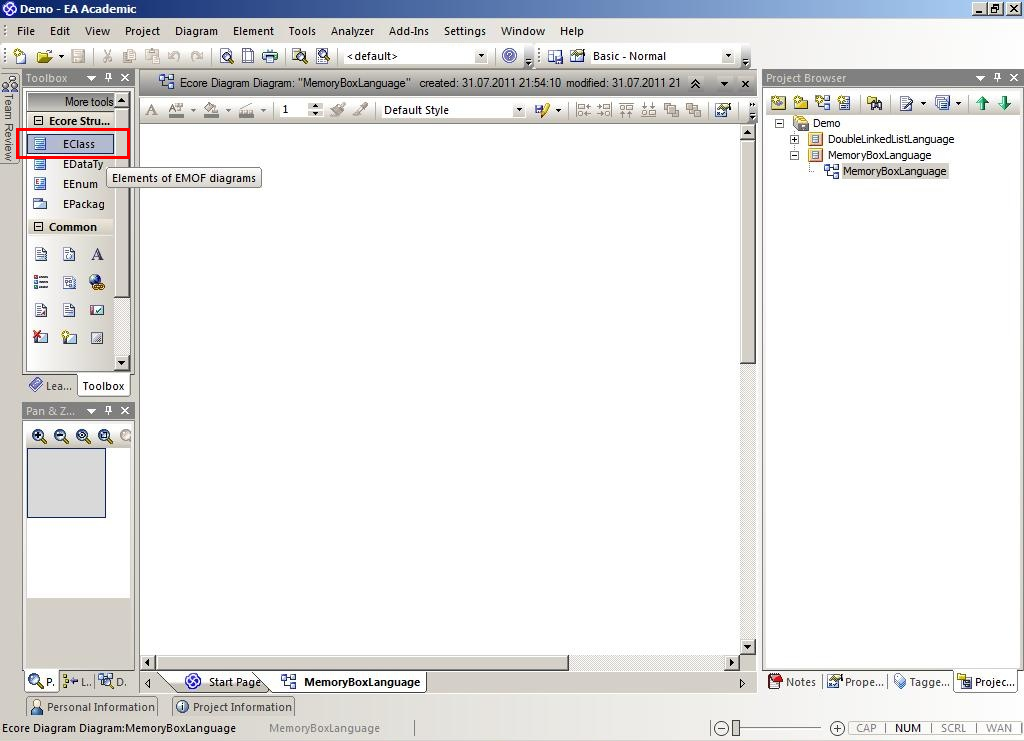
\includegraphics[width=0.7\textwidth]{pics/memBox07.png}
	\caption{Create an EClass.}
	\label{fig:eclass}
\end{figure}

\clearpage

In the dialogue that pops-up, enter \texttt{Box} as the name of the class and
click \texttt{OK} (Fig.~\ref{fig:eclass_properties}).  This dialogue can
always be invoked by double-clicking the class and contains many other
properties we'll be looking into later in the tutorial.  In general, a similar
``properties'' dialogue can be opened in the same fashion for almost every
element in EA.

\begin{figure}[htbp]
	\centering
  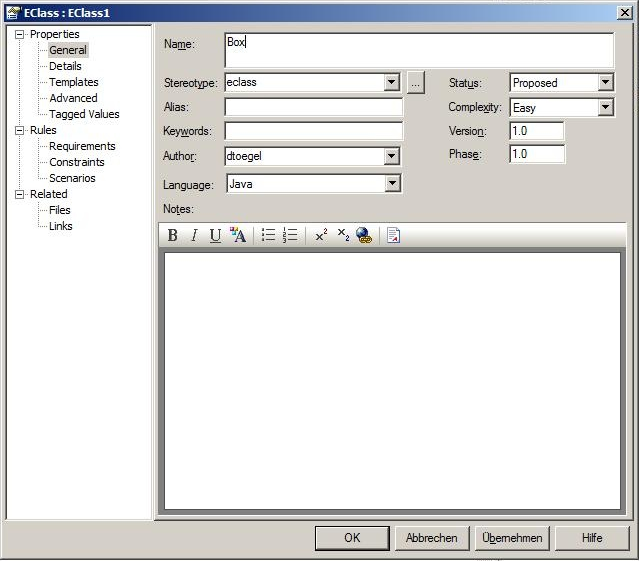
\includegraphics[width=0.6\textwidth]{pics/memBox08.png}
	\caption{Enter properties of EClass.}
	\label{fig:eclass_properties}
\end{figure}

After creating \texttt{Box}, your EA workspace should resemble
Fig.~\ref{fig:eclass_completed}. 

\begin{figure}[htbp]
	\centering
  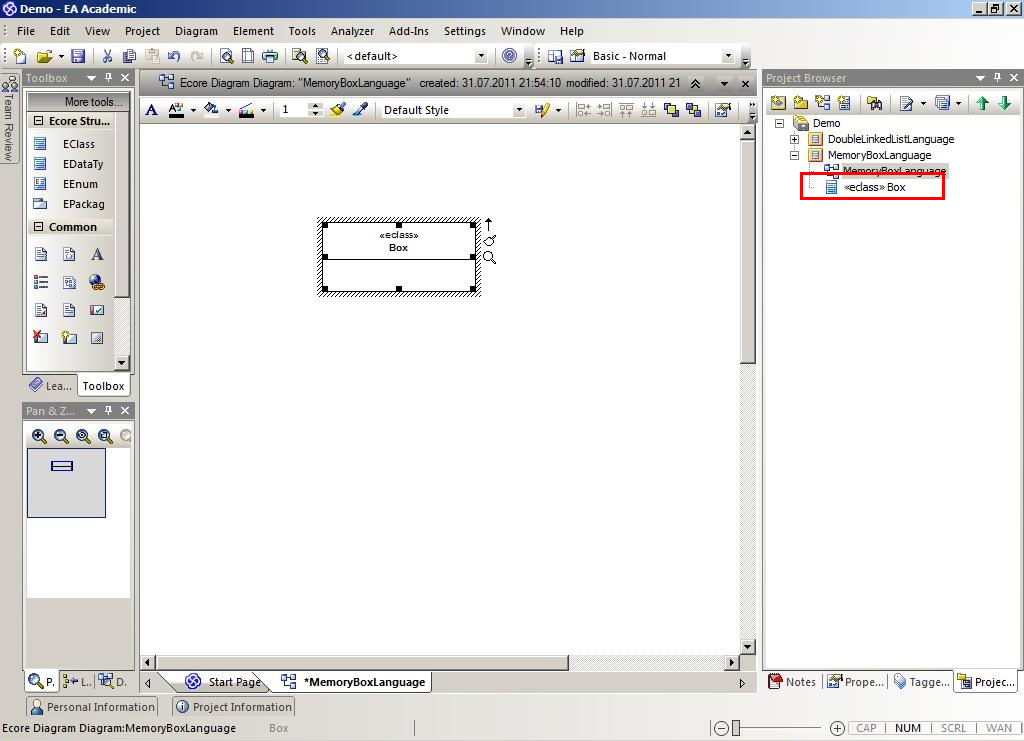
\includegraphics[width=0.7\textwidth]{pics/memBox09.png}
	\caption{State after creating \texttt{Box}.}
	\label{fig:eclass_completed}
\end{figure}

\clearpage

Now create \texttt{Partition} and \texttt{Card} in the same way, till your
workspace resembles Fig.~\ref{fig:all_eclasses}.  These are the main classes for
our memory box.

\begin{figure}[htbp]
	\centering
  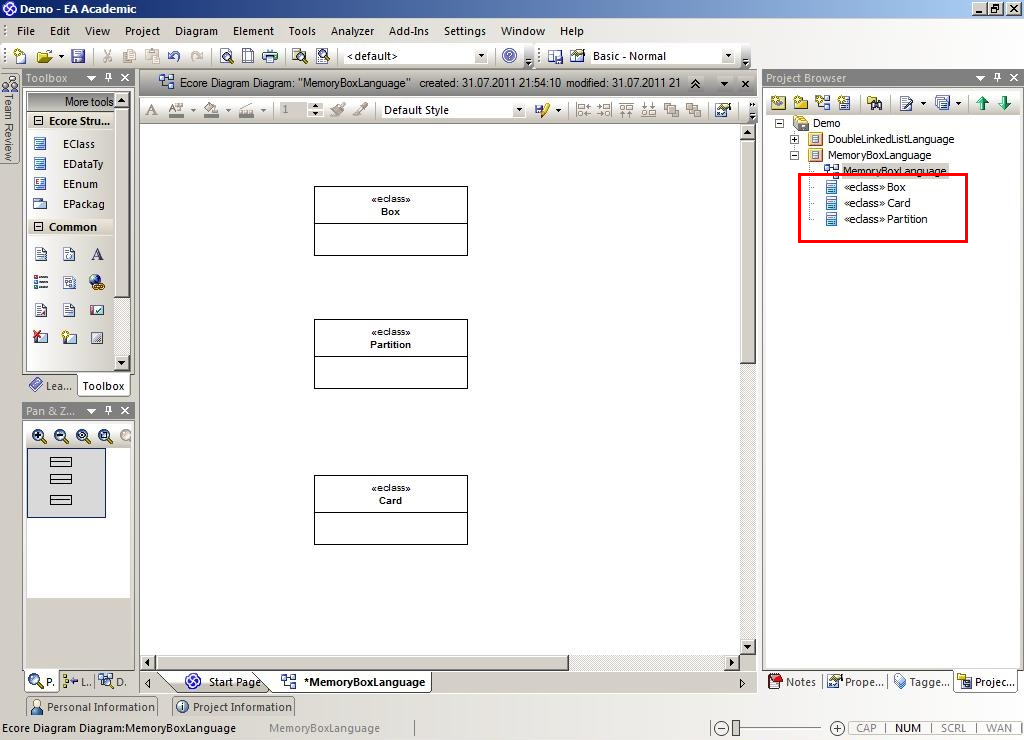
\includegraphics[width=0.7\textwidth]{pics/memBox10.png}
	\caption{Main classes in our metamodel.}
	\label{fig:all_eclasses}
\end{figure}

Now choose \texttt{Box}, right-click to call up the context menu and choose
\texttt{Att\-ri\-butes\ldots} (Fig.~\ref{fig:attribute}).

\begin{figure}[htbp]
	\centering
  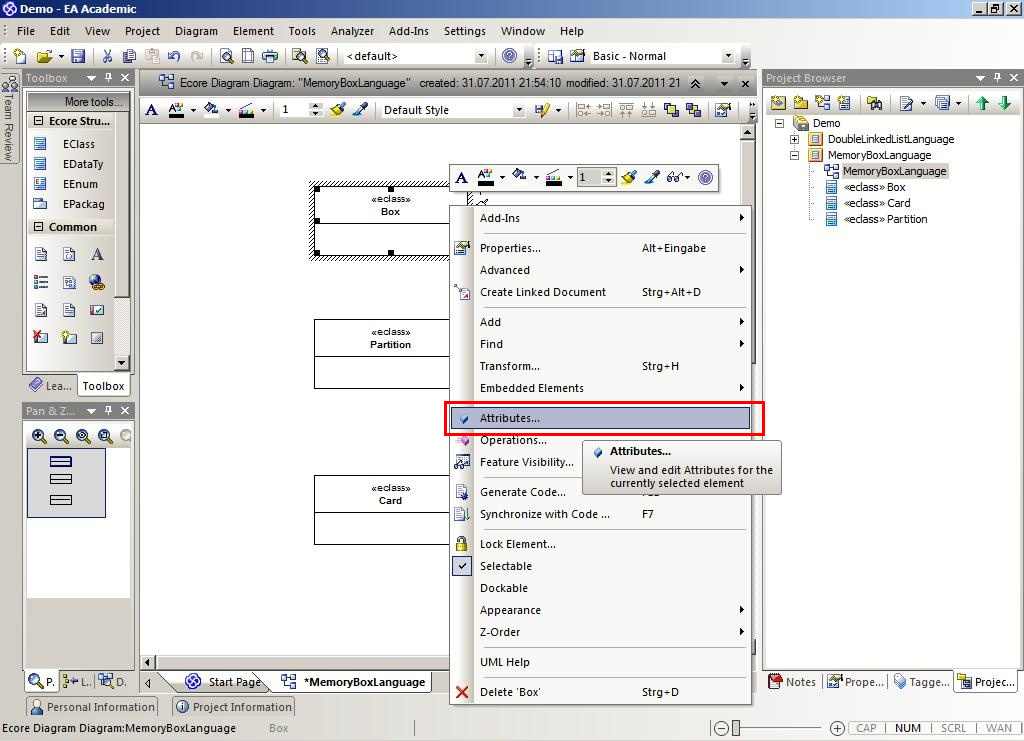
\includegraphics[width=0.7\textwidth]{pics/memBox11.png}
	\caption{Context Menu for a class.}
	\label{fig:attribute}
\end{figure}

\clearpage

In the dialogue that pops-up, enter \texttt{name} as the name of the attribute,
choose \texttt{EString} as its type and press \texttt{Save}
(Fig.~\ref{fig:attribute_properties}).  A new attribute for the same class can
be added by choosing \texttt{New}.

\begin{figure}[htbp]
	\centering
  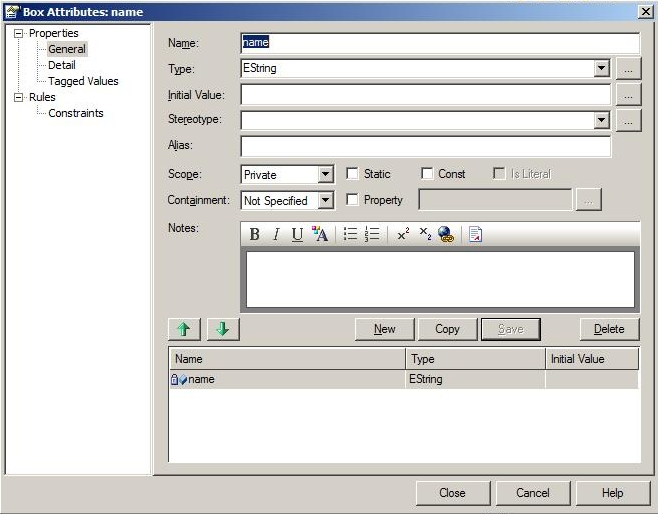
\includegraphics[width=0.7\textwidth]{pics/memBox13.png}
	\caption{Adding attributes to a class.}
	\label{fig:attribute_properties}
\end{figure} 

Add attributes to the other classes till your workspace resembles
Fig.~\ref{fig:attribute_completed}.

\begin{figure}[htbp]
	\centering
  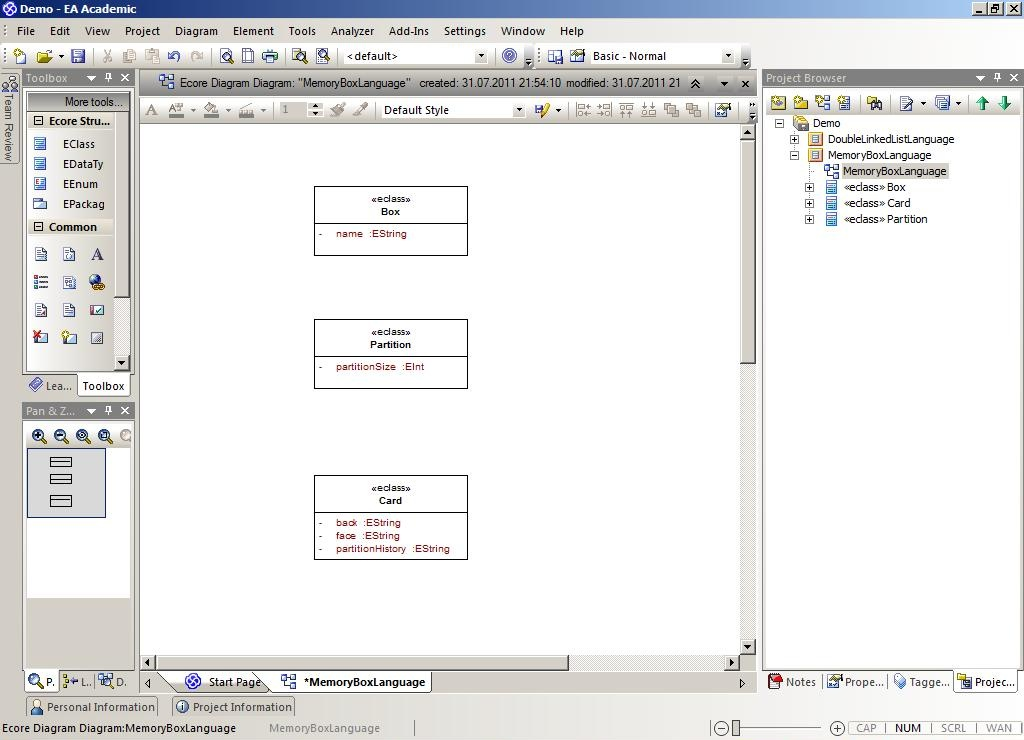
\includegraphics[width=0.73\textwidth]{pics/memBox14.png}
	\caption{Main classes with attributes.}
	\label{fig:attribute_completed}
\end{figure}

\clearpage

Now choose \texttt{EPackage} from the toolbox and add it to the current diagram
just like how we added EClasses. Enter \texttt{facade} as the name of the
package. 

Ecore supports packages that can be used to structure and group classes
in a metamodel.  In our case, we need  a util class that implements helper
methods for our memory box.  These methods  will be implemented by hand in Java
and the util class thus represents a kind of  interface or ``facade'' between
our model and hand-written code.  We shall soon  see how our Eclipse Plugin
offers extra support if one follows this naming  convention for packages
containing hand-written code. 

To add a class to our new package, select it in the Project Browser and then
press the button \texttt{Create Element} (Fig.~\ref{fig:epackage_newelement}).  

\begin{figure}[htbp]
	\centering
  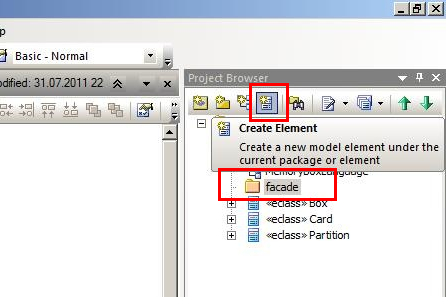
\includegraphics[width=0.6\textwidth]{pics/memBox19.png}
	\caption{Add a class to the package.}
	\label{fig:epackage_newelement}
\end{figure}

In the dialogue that pops-up, the correct toolbox should be preselected.  Enter
\texttt{MemoryBoxUtil} as the name of the class and click \texttt{Create}
(Fig.~\ref{fig:epackage_createelement}).

\begin{figure}[htbp]
	\centering
  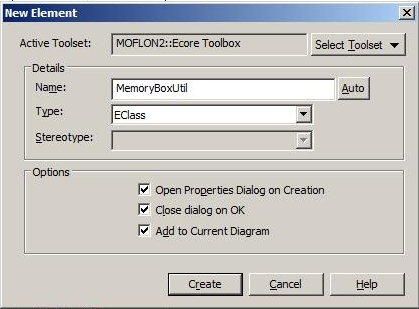
\includegraphics[width=0.5\textwidth]{pics/memBox20.png}
	\caption{Enter name of class to create.}
	\label{fig:epackage_createelement}
\end{figure}

\clearpage

Your workspace should now resemble Fig.~\ref{fig:epackage_completed}.  Every
subpackage like \texttt{facade} can also contain diagrams that can be created
and added using the Project Browser just like how we created the current
diagram. In this way an arbitrary nesting of packages is possible.

\begin{figure}[htbp]
	\centering
  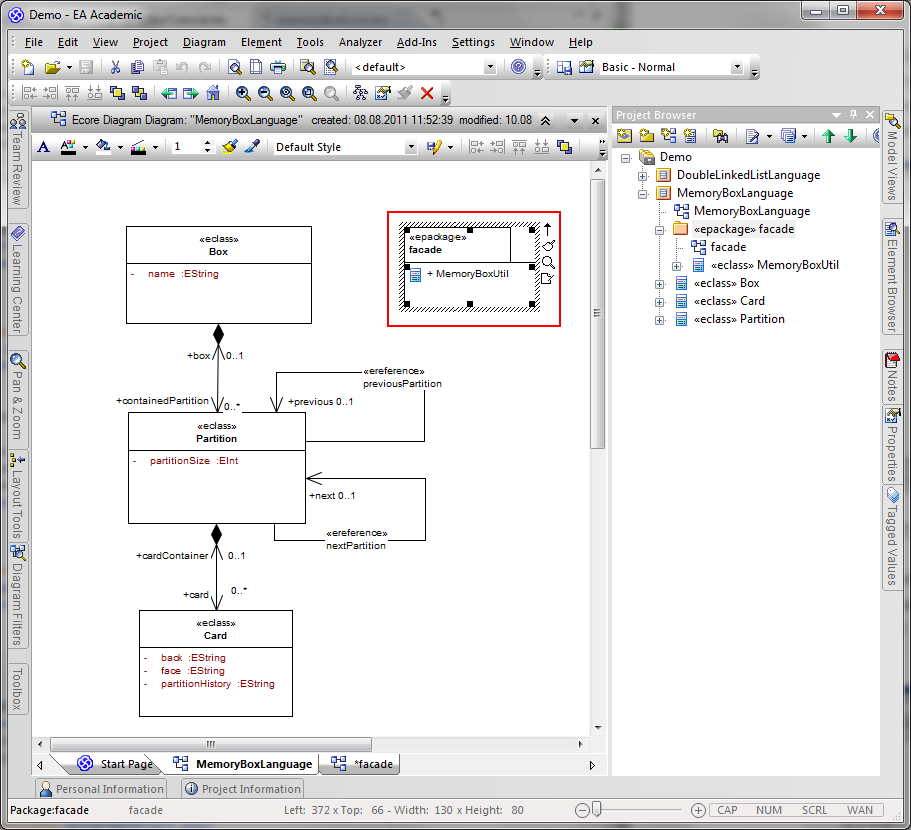
\includegraphics[width=0.7\textwidth]{pics/memBox22.png}
	\caption{Workspace after adding package.}
	\label{fig:epackage_completed}
\end{figure}

A fundamental gesture in EA is \emph{Quick Link}.  Quick Link is used to create
links between elements in a context sensitive manner.  To use Quick Link,
choose an element and note the little black arrow in its top-right corner
(Fig.~\ref{fig:quicklink}).

\begin{figure}[htbp]
	\centering
  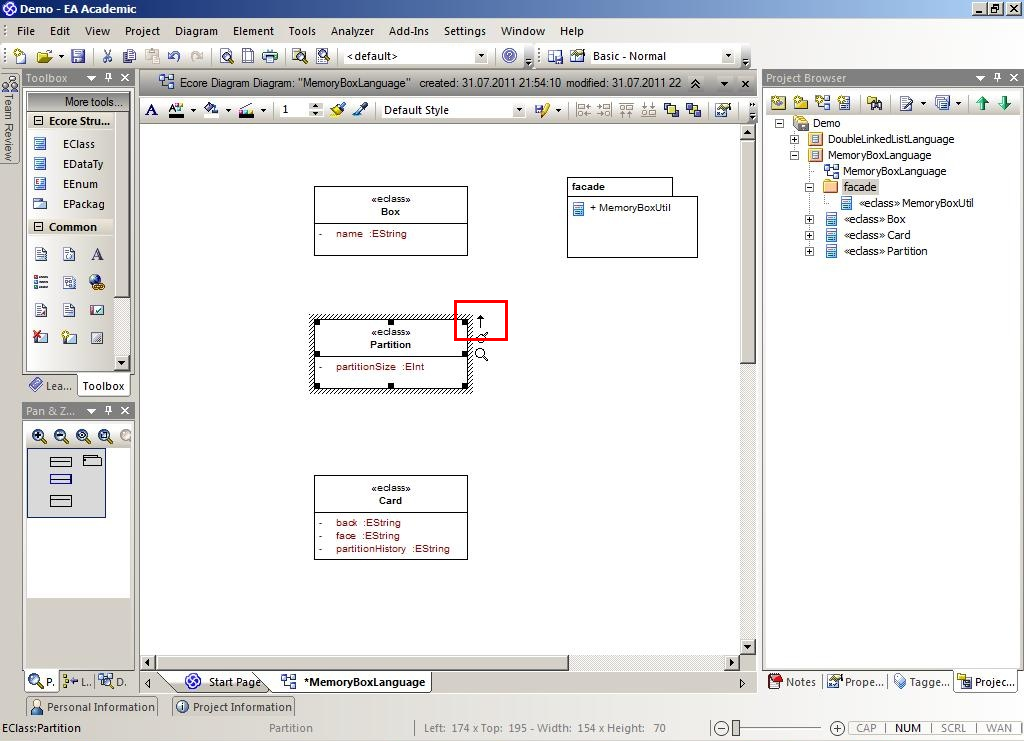
\includegraphics[width=0.7\textwidth]{pics/memBox23.png}
	\caption{Quick Link is a central gesture in EA.}
	\label{fig:quicklink}
\end{figure}

\clearpage

Now click on the black arrow and pull to another element you wish to ``quick
link" to.  In this case quick link from \texttt{Partition} to \texttt{Box}.  In
the context-menu that pops-up, choose \texttt{EReference}.
(Fig.~\ref{fig:ereference}). 

\begin{figure}[htbp]
	\centering
  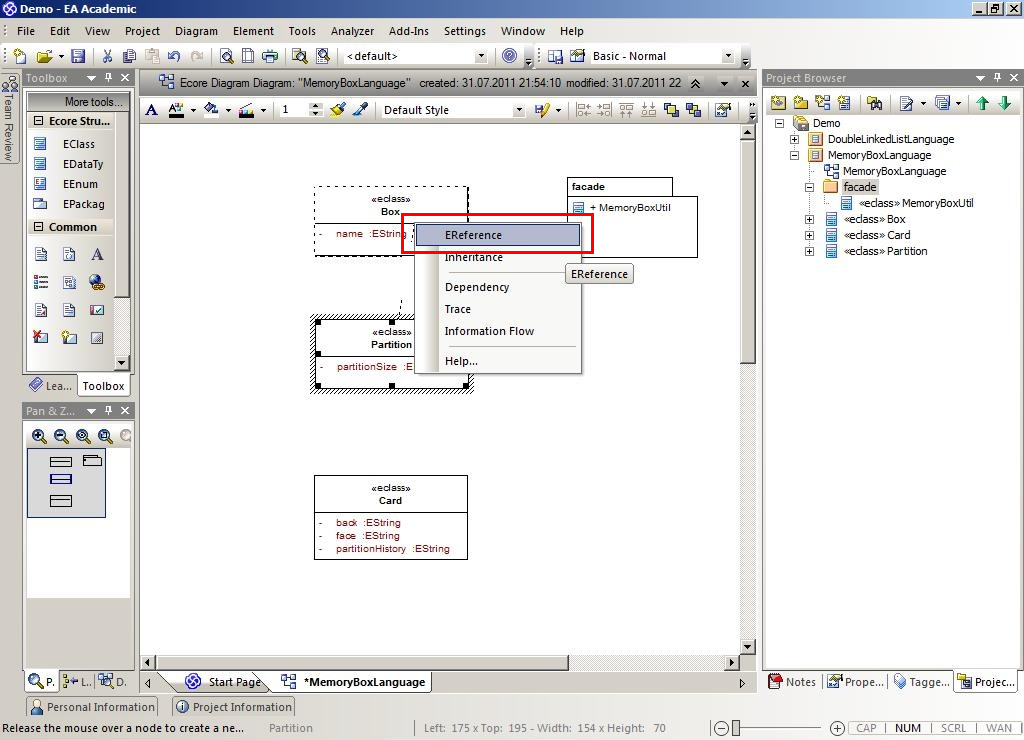
\includegraphics[width=0.6\textwidth]{pics/memBox24.png}
	\caption{Create a reference via Quick Link.}
	\label{fig:ereference}
\end{figure}

In the dialogue that pops-up (Fig.~\ref{fig:ereference_properties}), the
direction of the reference can be set.  The default is bidirectional and this is
ok for our \texttt{Box}-\texttt{Partition} connection.  A \texttt{Name} can also
be entered, which is only used for documentation purposes and is not relevant
for codegeneration.

\begin{figure}[htbp]
	\centering
  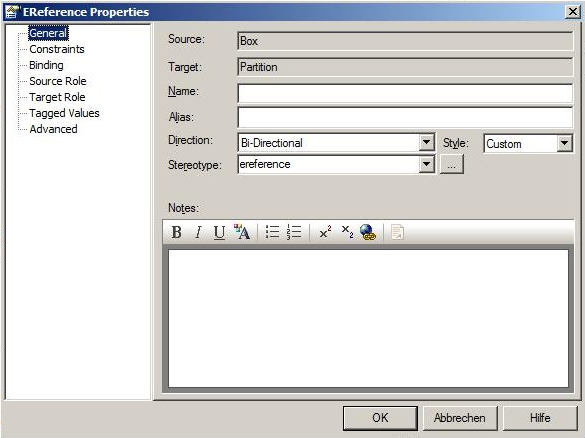
\includegraphics[width=0.6\textwidth]{pics/memBox25.png}
	\caption{Enter properties of the reference.}
	\label{fig:ereference_properties}
\end{figure}
	
\clearpage

In the same dialogue choose \texttt{Source Role} and enter the values in
Fig.~\ref{fig:ereference_properties} to set the properties for the ``source''
end of the reference (the \texttt{Box} role).  Important is a name for the role
(\texttt{box}), the \texttt{Multiplicity}, \texttt{Aggregation} and
\texttt{Navigability}.  Repeat the process for the \texttt{Target Role}.
  
\begin{figure}[htbp]
	\centering
  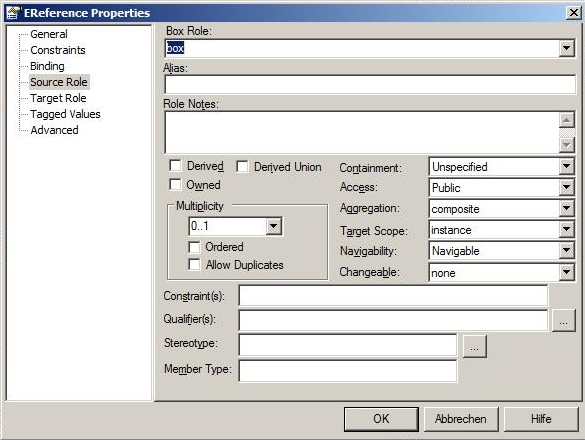
\includegraphics[width=0.5\textwidth]{pics/memBox26.png}\\
  \vspace{0.5cm}
  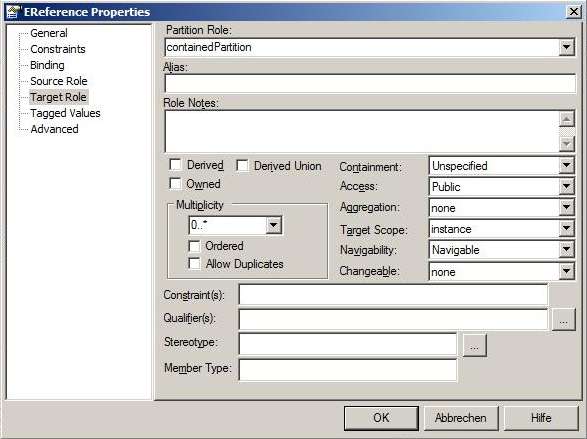
\includegraphics[width=0.5\textwidth]{pics/memBox27.png}
	\caption{Enter properties for source and target of reference.}
	\label{fig:reference_ends}
\end{figure}

Navigable ends are mapped to class attributes with getters and setters in Java
and therefore \emph{must} have a specified name and  multiplicity for successful
codegeneration.  
Corresponding Values for non-navigable ends can  be regarded as additional
documentation and do not have to be specified.
 
The multiplicity of a reference controls if the relation is mapped to a Java
Collection (\texttt{*},  \texttt{1..*}, \texttt{0..*}), or a single valued class
attribute (\texttt{1}, \texttt{0..1}).

In Ecore, the aggregation values of a reference can either be \texttt{none} or
\texttt{com\-po\-site}.  Composite means that the current role is that of a
\emph{container} for the opposite role.  In our case for example, \texttt{box}
is a container for \texttt{partitions}.\\  This has a series of
consequences: (1) every element must have a container, (2) an element cannot be
in more than one container at the same time, and (3) a container's contents are
deleted together with the container.  Non-composite (\texttt{none}) means that
the current role is not that of a container and the rules for containment do not
hold (reference is a simple ``pointer'').

\clearpage

If you've done everything right, your workspace should now resemble
Fig.~\ref{fig:ereference_completed} with a relation between \texttt{Box} and
\texttt{Partition}.

\begin{figure}[htbp]
	\centering
  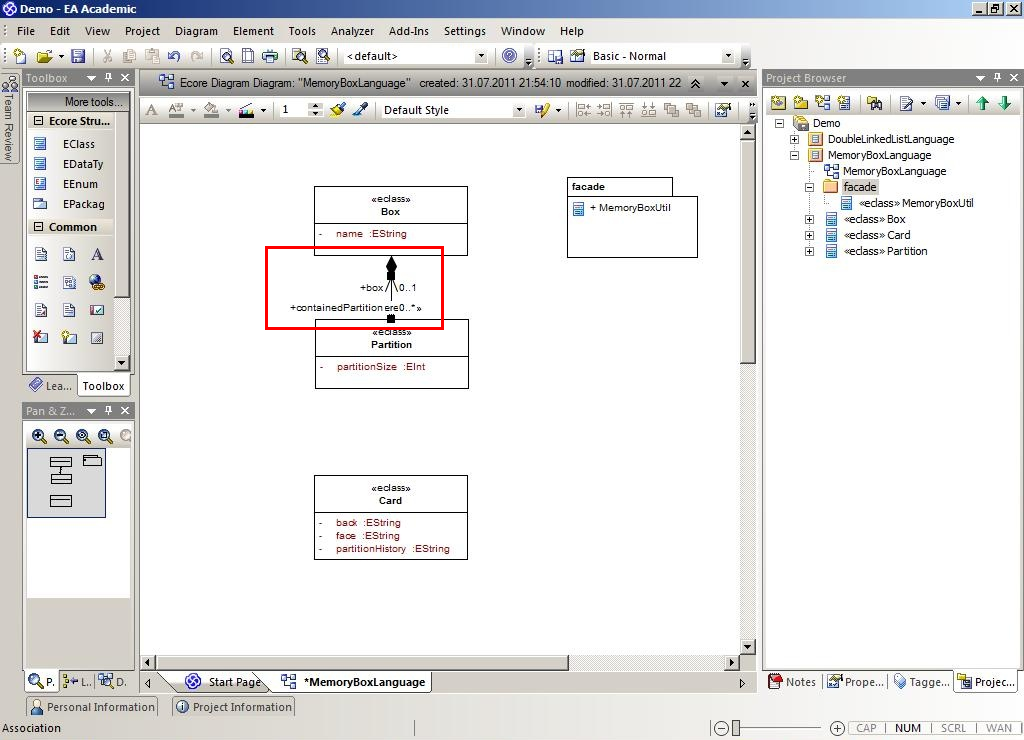
\includegraphics[width=0.7\textwidth]{pics/memBox28.png}
	\caption{\texttt{Box} contains \texttt{Partition}s.}
	\label{fig:ereference_completed}
\end{figure}

Create a bidirectional reference\footnote{To be precise, \emph{all} references
in Ecore are actually unidirectional.  A ``bidirectional'' reference in our
metamodel is in reality mapped to two \texttt{EReferences} that are opposites of
each other.  
We however believe it is simpler to handle these pairs as single references and
prefer this concise concrete syntax.} between \texttt{Partition} and \texttt{Card}
and two unidirectional self-references for \texttt{Partition} according to
Fig.~\ref{fig:ereferences_all}.
 
\begin{figure}[htbp]
	\centering
  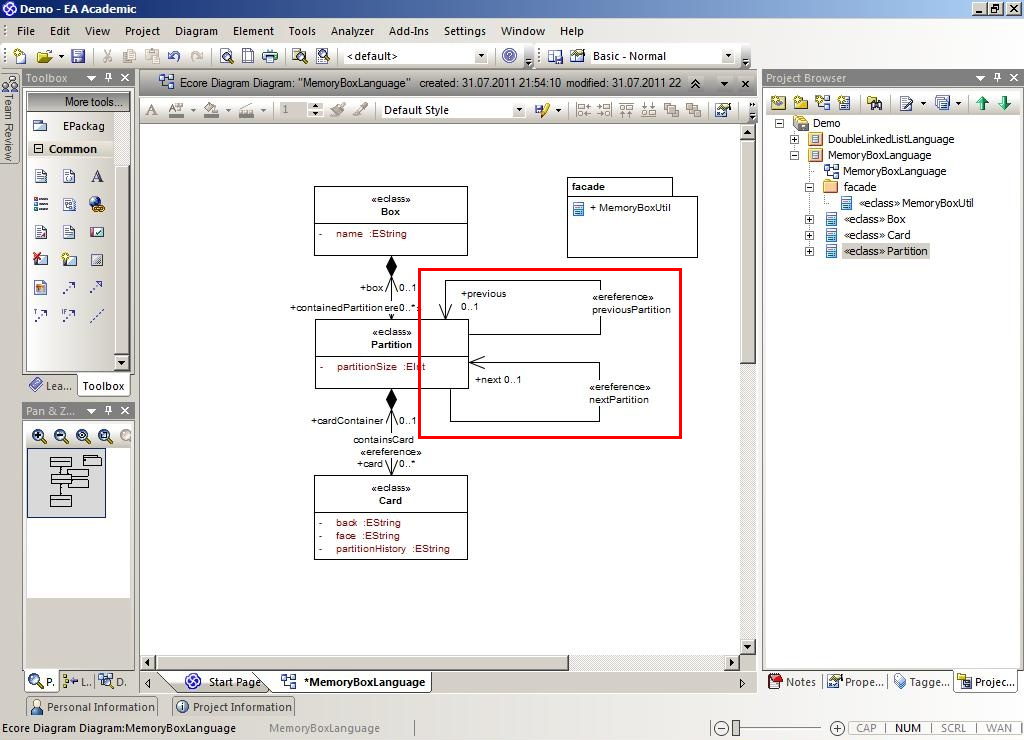
\includegraphics[width=0.7\textwidth]{pics/memBox34.png}
	\caption{All relations in our metamodel.}
	\label{fig:ereferences_all}
\end{figure}

\clearpage

Every system has, in addition to its static structure, certain dynamic aspects
that describe the system's behaviour and how it evolves over time or reacts to
external stimulus.
\marginpar{\emph{Dynamic Semantics}}
In a language, these rules that govern the dynamic behaviour of a system are
referred to collectively as the \emph{Dynamic Semantics} of the language.  
Although these rules can be defined as a set of separate \emph{Model
Transformations}, we take a holistic approach and advocate integrating the
transformations directly in the metamodel as operations.
This fits nicely to the object oriented paradigm and is quite natural in many
cases.  In the next few steps we shall define the \emph{signatures} of some
operations for our memory box.  We will of course use SDMs to \emph{implement}
the methods later.

Right-click \texttt{Partition} to invoke the context-menu depicted in
Fig.~\ref{fig:add_operation} and choose \texttt{Operations\ldots}.

\begin{figure}[htbp]
	\centering
  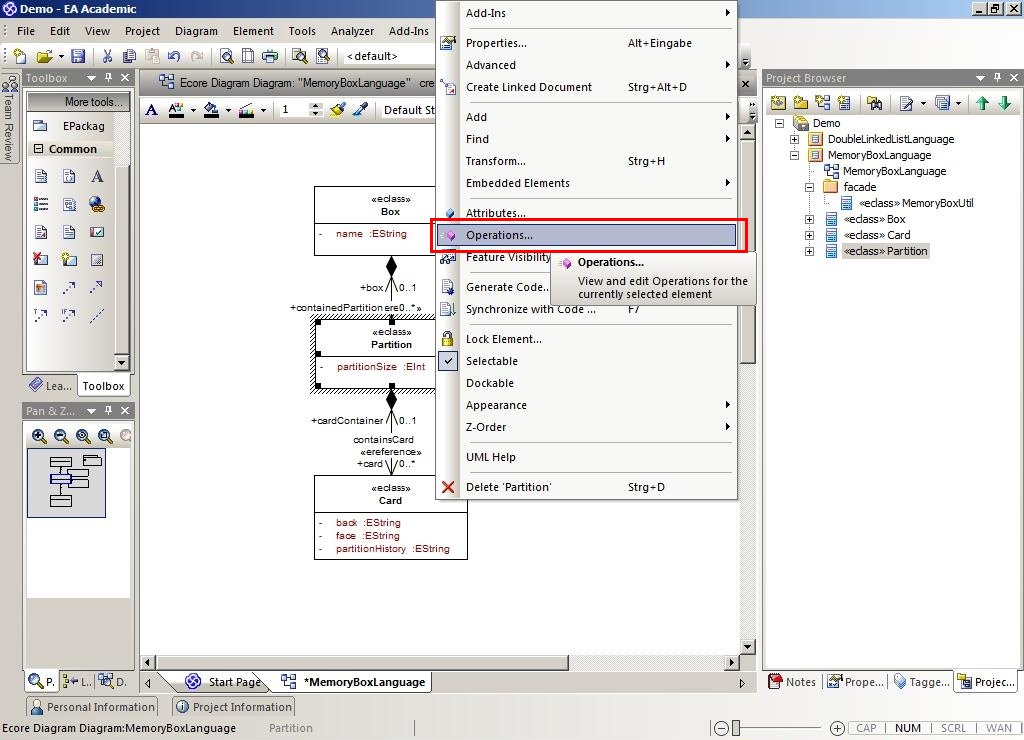
\includegraphics[width=0.6\textwidth]{pics/memBox35.png}
	\caption{Add an operation.}
	\label{fig:add_operation}
\end{figure}
 
In the dialogue that pops-up (Fig.~\ref{fig:operation_properties}), enter
\texttt{empty} as the \texttt{Name} of the operation, leave the \texttt{Return
Type} as \texttt{void}.  Press \texttt{Save}.
 
\begin{figure}[htbp]
	\centering
  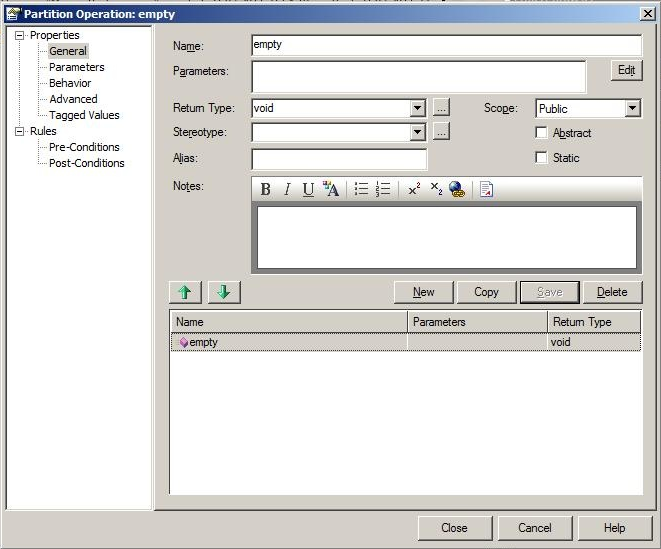
\includegraphics[width=0.45\textwidth]{pics/memBox37.png}
	\caption{Properties for operation.}
	\label{fig:operation_properties}
\end{figure}

\clearpage

In the same dialogue, press \texttt{New} to add further operations and enter the
values in Fig.~\ref{fig:operation_parameters}.  Parameters can be added by
pressing \texttt{Edit} and entering the name and choosing the type of each
Parameter in a separate dialogue.

\begin{figure}[htbp]
	\centering
  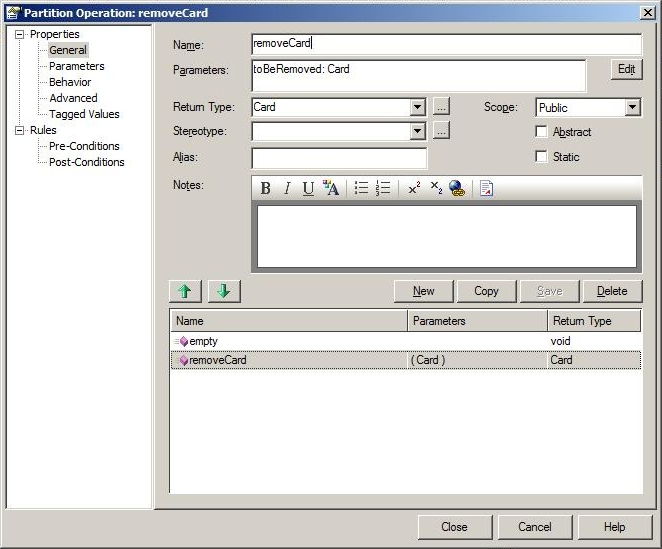
\includegraphics[width=0.6\textwidth]{pics/memBox38.png}
	\caption{Parameters and Return Type.}
	\label{fig:operation_parameters}
\end{figure}

Repeat the process for the values in Fig.~\ref{fig:operation_partition}.  The
\texttt{Return Type} can be chosen via the drop-down menu for primitives
(\texttt{EBoolean}), or via the \texttt{\ldots} button for types in the
metamodel (\texttt{Card}). 

If you've done everything right, your dialogue should
now contain three methods \texttt{check}, \texttt{empty}, and
\texttt{removeCard} with corresponding parameters and return types as in
Fig.~\ref{fig:operation_partition}.

\begin{figure}[htbp]
	\centering
  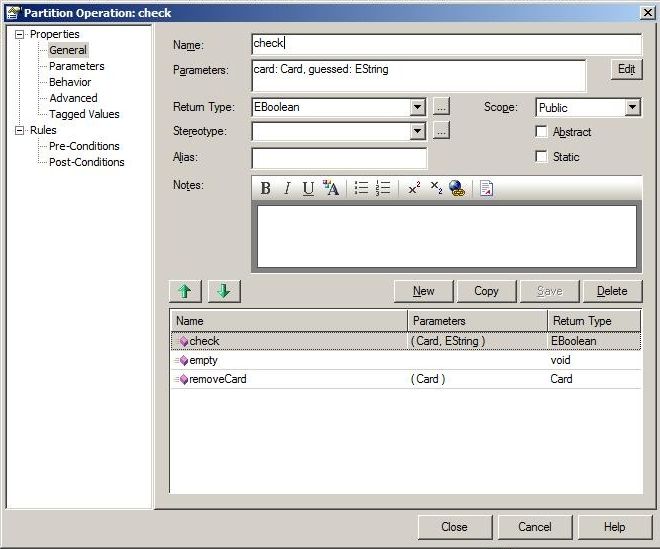
\includegraphics[width=0.6\textwidth]{pics/memBox39}
	\caption{All operations in \texttt{Partition}.}
	\label{fig:operation_partition}
\end{figure}

\clearpage

Add all operations analogously for \texttt{Box} and \texttt{Card} so that your
metamodel closely resembles Fig.~\ref{fig:metamodel_complete}.
 
\begin{figure}[htbp]
	\centering 
  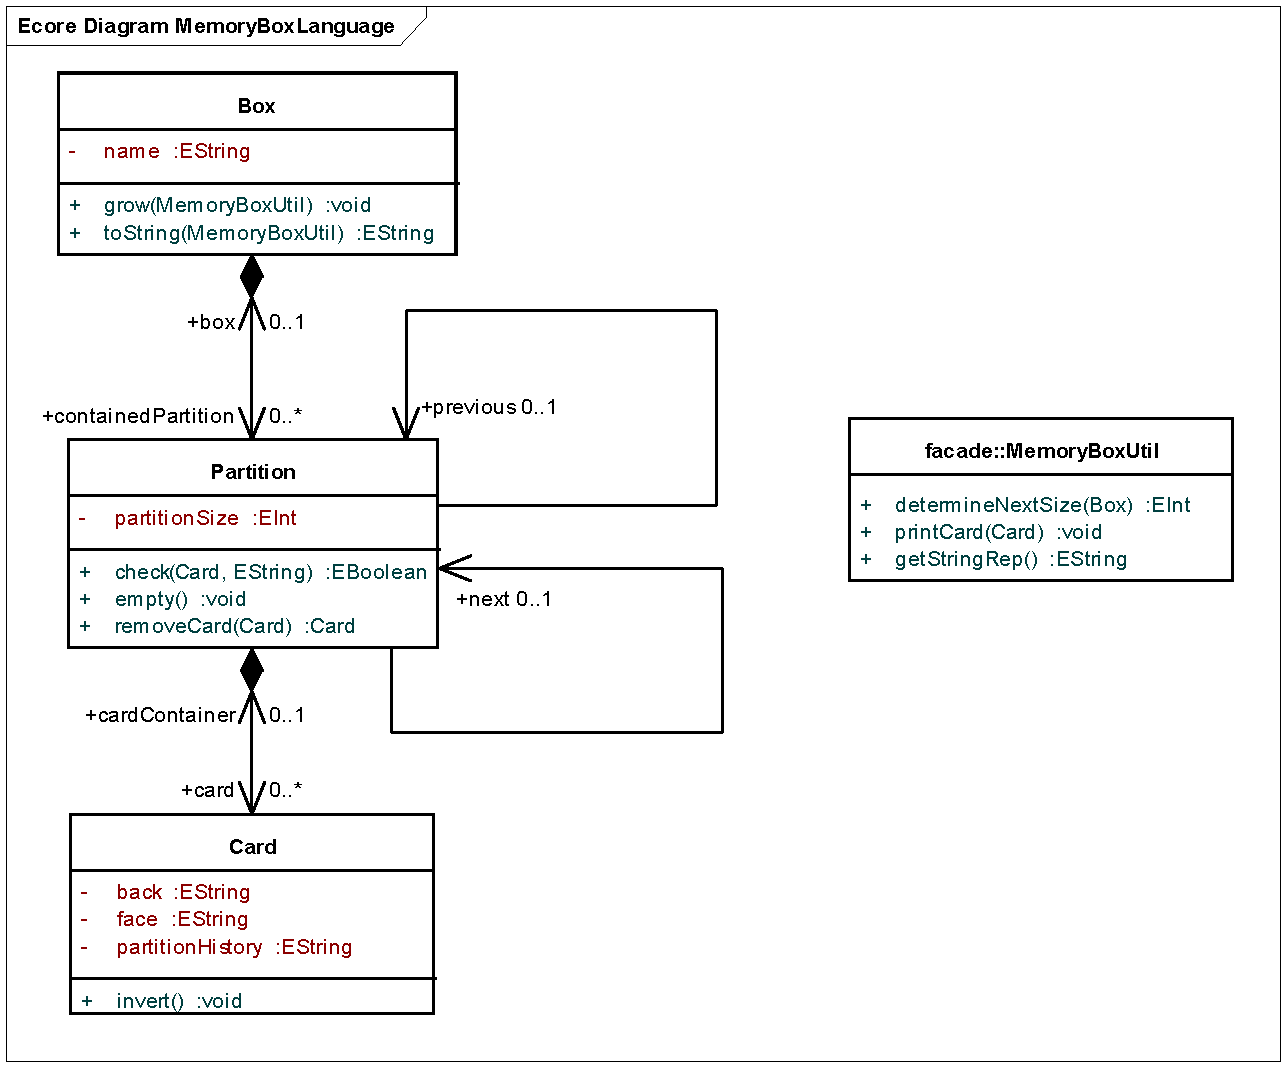
\includegraphics[width=\textwidth]{pics/memBox44} 
	\caption{Complete metamodel for our memory box.}
	\label{fig:metamodel_complete}
\end{figure}

Lets take a step back and review our metamodel.  We have modelled a \texttt{Box}
that contains arbitrary many \texttt{Partition}s.  A \texttt{Partition} in the
\texttt{Box} has a \texttt{next} and \texttt{previous} \texttt{Partition} that
can be set or not. Finally, \texttt{Partition}s contain \texttt{Card}s.

A \texttt{Box} has a \texttt{name}, and can be extended by calling
\texttt{grow}. A \texttt{Box} can print out its contents via \texttt{toString}. 
We'll see later in the tutorial why these two methods need our
\texttt{MemoryBoxUtil} as a parameter.

The main method of the memory box is \texttt{Partition::check} that takes a
\texttt{Card} and the user's guess as an \texttt{EString} and returns
\texttt{true} or \texttt{false} depending on if the guess was correct or not.
A \texttt{Partition} can also \texttt{empty} itself of all \texttt{Cards}, or
\texttt{remove} a particular \texttt{Card}.  Last but not least, a
\texttt{Partition} has a \texttt{partitionSize} that can be used to indicate
that the \texttt{Partition} is full and is ready to be revised.

\clearpage

A \texttt{Card} contains the actual content to be learnt as a question on the
card's \texttt{face} and the answer on the card's \texttt{back}. A \texttt{Card}
also maintains a \texttt{partition\-History} which can be used to keep track of
how often a \texttt{Card} has been answered correctly/wrongly.  This might
indicate how difficult the \texttt{Card} is for a specific user.
When learning a language, it makes sense to be able to swap the target and
source langauge and this is supported by \texttt{Card} via \texttt{invert}
(turns the card around).

Now try to export the metamodel for codegeneration in Eclipse.  To do this
right-click on \texttt{MemoryBoxLanguage} and choose ``Add-In/MOFLON::Ecore
Addin/Export Selection to Workspace''.  Then switch to your Eclipse workspace
and refresh the metamodel workspace.

If you have done everything right, a new project \texttt{MemoryBoxLanguage}
should be created in the \texttt{Demo} working set in your Eclipse workspace.
If this is not the case please ensure that your metamodel is identical with
Fig.~\ref{fig:metamodel_complete}.  If you believe everything is correct and
things still don't work then feel free to contact us at
\url{contact@moflon.org}.  If code is generated successfully, take a look at all
the stuff that has been generated under \texttt{/gen}, especially the default
implementation for all methods that just throws an
\texttt{OperationNotSupported} exception.  We shall see later in the tutorial
that the EMF codegenerator actually supports merging hand-written
implementations of methods with generated code.  With eMoflon however, we can
also model a large part of the dynamic semantics and only need to implement
small helper methods for e.g. string manipulation by hand.

Let's move on and model the dynamic behaviour of our memory box!
\section{Dynamic Semantics with SDM}
\label{sec:sdm_intro}

The core idea when modelling behaviour is to regard dynamic aspects of a system
(let's call this a model as from now on) as bringing about a change of
state.
This means a model in state $S$ can evolve to state $S^*$ via a
transformation $\Delta: S \stackrel{\Delta}{\rightarrow}S^*$.
In this light, dynamic or behavioural aspects of a model are synonymous with
\emph{model transformations}, and the dynamic semantics of a language equate
simply to a suitable set of model transformations.
This approach is once again quite similar to OO where objects have state and can
\emph{do} things via methods that manipulate their state.        

So how do we model model transformations?  There are quite a few possibilities.
We could employ a suitably concise imperative programming language with which we
simply say in a step-by-step manner how the system morphs.
There actually exist quite a few very successful languages and tools in this
direction.

But isn't this almost like just programming directly in Java?
There must be a better way to do this\ldots  From the relatively mature
area of graph grammars and graph transformations we take a \emph{declarative}
and \emph{rule-based} approach.  
Declarative in this context means that we do not want to specify exactly how and
in what order changes to the model must be carried out to achieve a
transformation. 
We just want to say under what conditions the transformation can be executed
(precondition), and the state of the model after executing the transformation
(post condition). 
The actual task of going from precondition to postcondition should  be taken
over by a transformation engine and all related details are basically regarded
as a black box.         

Ok - so a model transformation is of the form $(pre, post)$.  Inspired by string 
grammars, let's call this black box transformation a \emph{rule}, and
consequently the precondition the left-hand side of the rule $L$ and the
postcondition the right-hand side $R$.  

A rule $r: (L,R)$ can be \emph{applied} to a model (a typed graph) $G$ by:
\begin{enumerate}
  \item Finding an occurrence of the precondition $L$ in $G$ via a \emph{match}
  $m$,
  \item Cutting out $Destroy := (L\setminus R)$ i.e., the elements that are
  present in the precondition but not in the postcondition are to be deleted,
  from $G$ to form  $(G\setminus Destroy)$ and
  \item Pasting $Create := (R\setminus L)$ i.e., new elements that are
  present in the postcondition but not in the precondition and are to be
  created, into the hole in $(G\setminus Destroy)$ to form a new graph $H =
  (G\setminus Destroy) \cup Create$.
\end{enumerate}

Rule application is denoted as $G \stackrel{r}{\Rightarrow} H$ and is depicted
in Fig.~\ref{fig:rule_application}. 

%\usepackage{graphics} is needed for \includegraphics
\begin{figure}[htp]
\begin{center}
  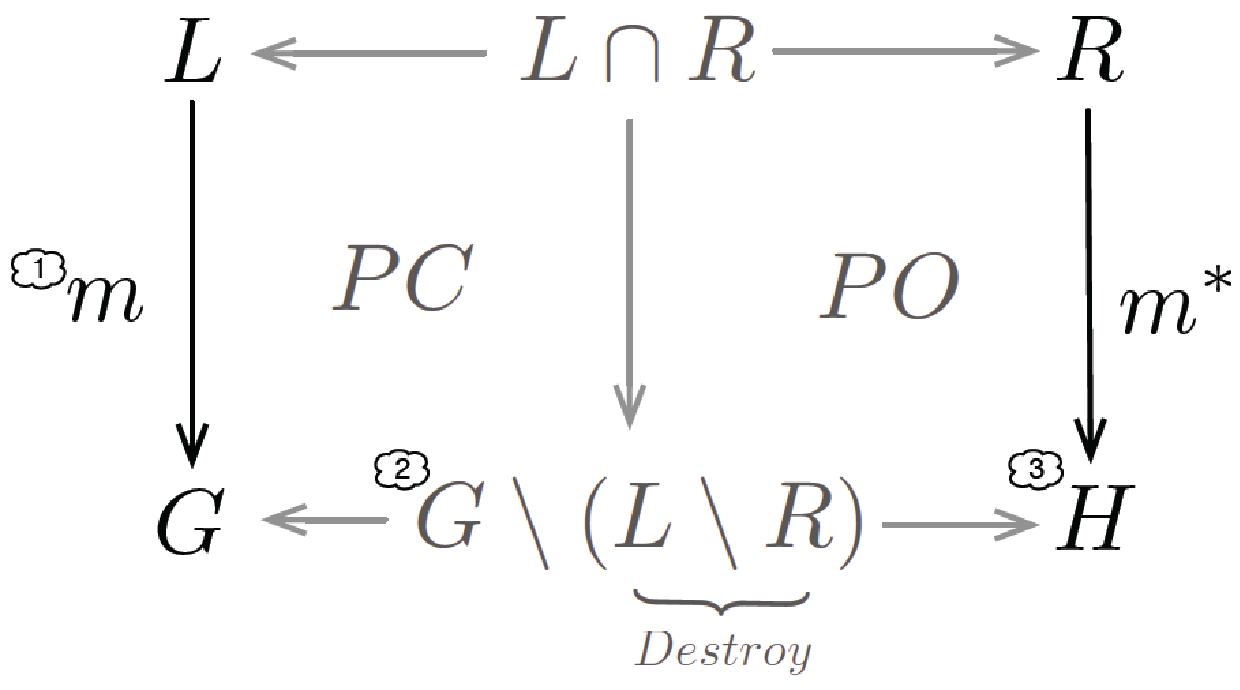
\includegraphics[width=0.6\textwidth]{pics/rule_application}
  \caption[]{Applying a rule $r: (L,R)$ to $G$ to yield $H$} 
  \label{fig:rule_application}
\end{center}
\end{figure}

(1) is called \emph{graph pattern matching}, (2) is called building a
\emph{push-out complement} $PC = (G\setminus Destroy)$, so that $L \cup
(G\setminus Destroy) = G$ and (3) is called building a \emph{push-out} $PO = H$,
so that $(G\setminus Destroy) \cup R = H$. A push-out is a generalised union
defined on typed graphs.  As we are dealing with graphs here, it is not such a
trivial task to define (1) -- (3) in precise terms with conditions when a rule
can be applied and not, and there exists substantial theory with exactly that
goal. As this formalisation of rule application involves two push-outs: one
(deletion) when cutting out $Destroy := (L\setminus R)$ from $G$ to yield
$(G\setminus Destroy)$, and one (creation) when inserting $Create := (R\setminus
L)$ in $(G\setminus Destroy)$ to yield $H$, this is referred to as a
\emph{double push-out}.  
We won't go into further details in this tutorial, but the interested reader can
refer to \cite{EEPT06} for the exciting details.  

Now that we know what rules are, let's take a look at a simple example for our
memory box. How would a rule look like for moving a card from one partition to
the next?  Fig.~\ref{fig:rule_example} depicts the rule $moveCard$.
  
%\usepackage{graphics} is needed for \includegraphics
\begin{figure}[htp]
\begin{center}
  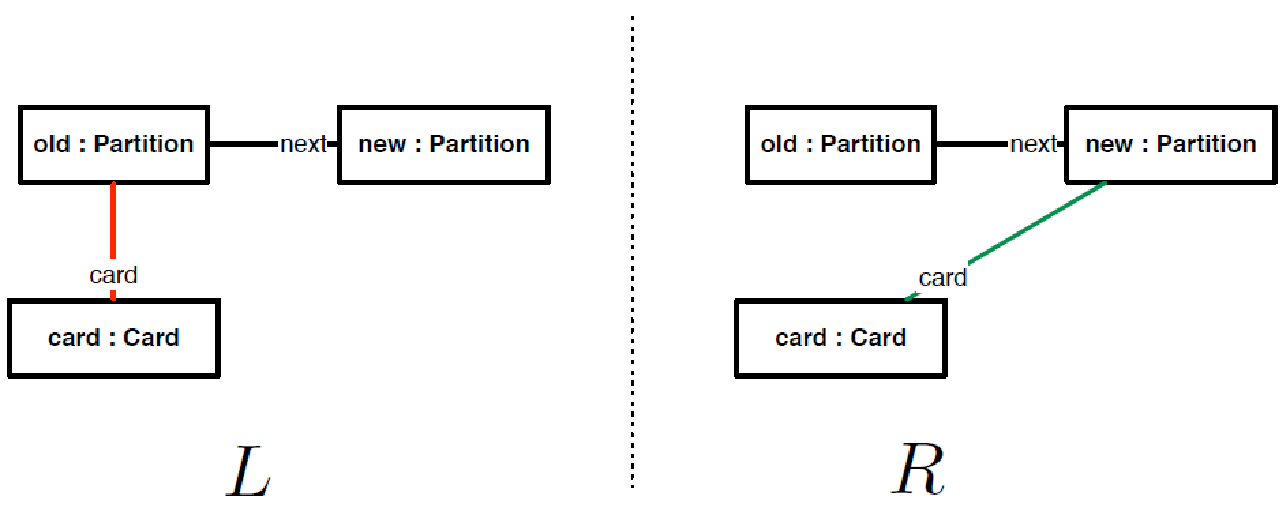
\includegraphics[width=0.9\textwidth]{pics/rule_example}
  \caption[]{Rule $moveCard$ as a graph transformation rule.}	
  \label{fig:rule_example}
\end{center}
\end{figure}

\clearpage

As already indicated by the colours used for $moveCard$ we employ a compact
representation of rules that is formed by merging $(L,R)$ into a single
\emph{story pattern} composed of  $Destroy := (L\setminus R)$ in red, $Retain := 
L\cap R$ in black, and $Create := (R\setminus L)$ in  green
(Fig.~\ref{fig:rule_compact}).
%\usepackage{graphics} is needed for \includegraphics
\begin{figure}[htp]
\begin{center}
  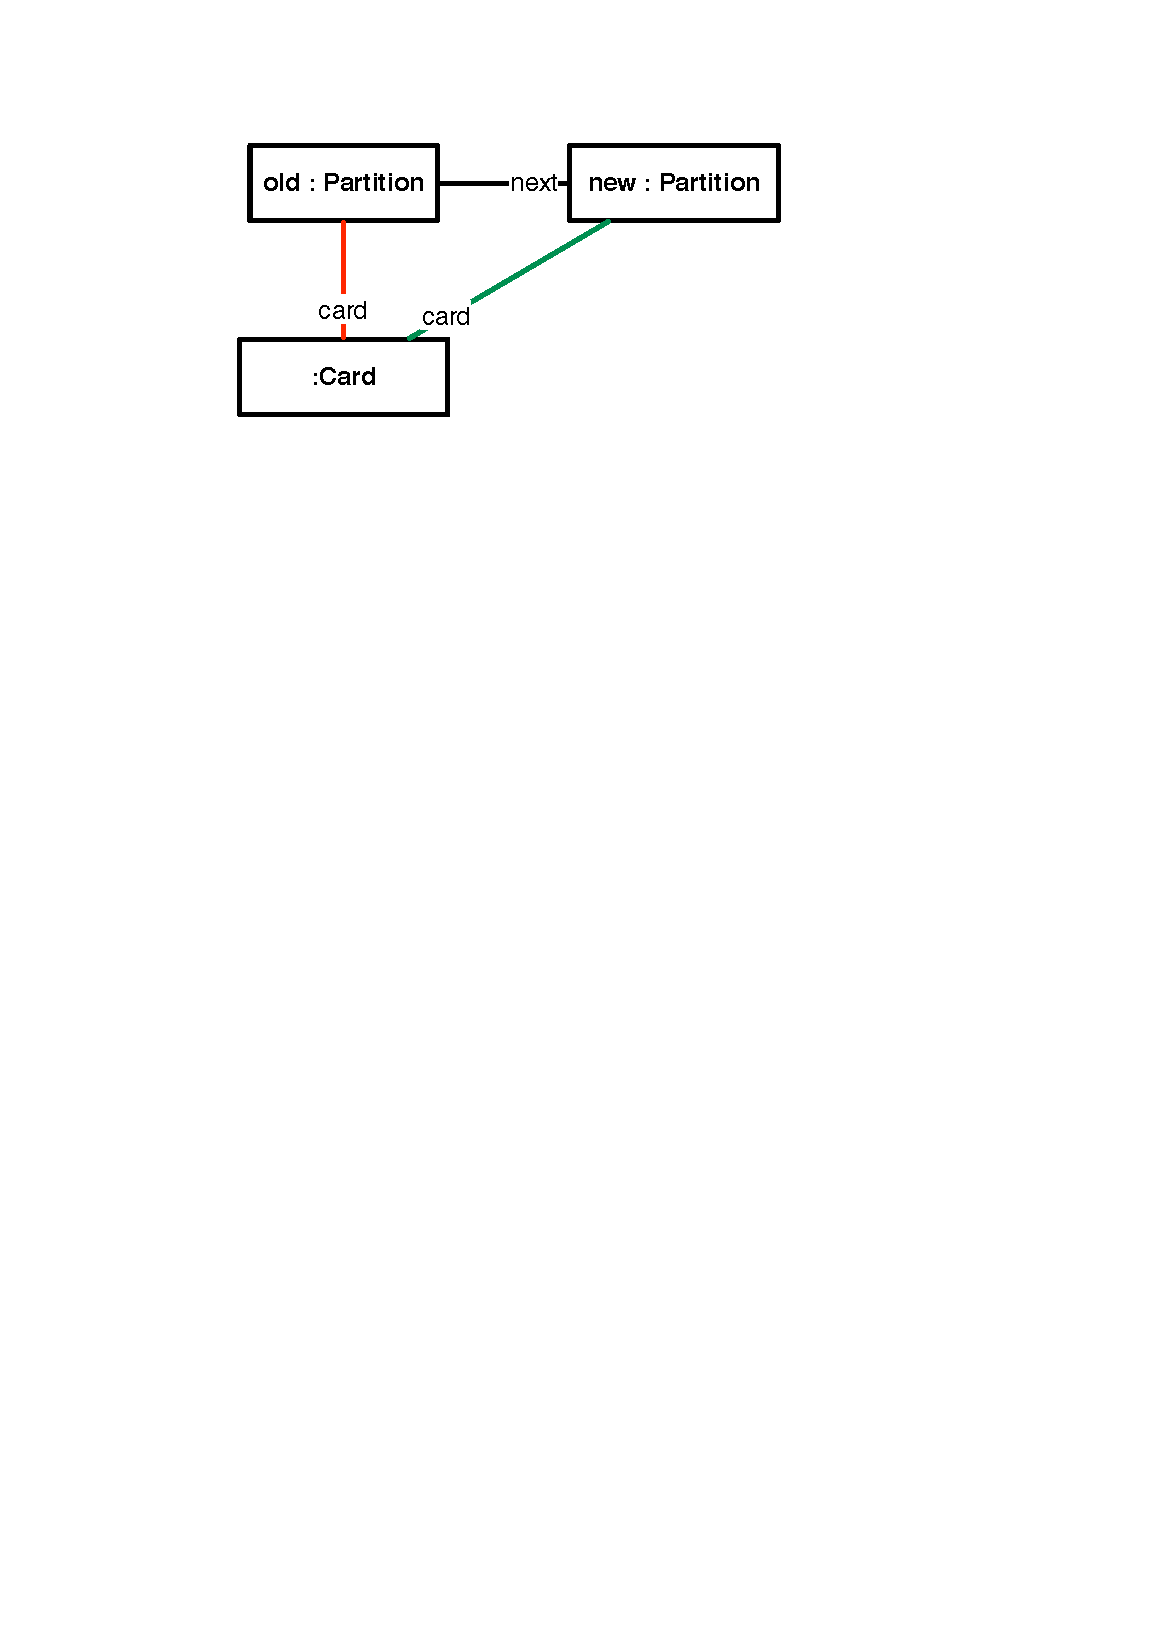
\includegraphics[width=0.45\textwidth]{pics/rule_compact}
  \caption[]{Compact representation of $moveCard$ as a Story Pattern.}
  \label{fig:rule_compact}
\end{center}
\end{figure}

 As we shall see in a moment, this  representation is quite intuitive and one can
just forget the details of rule application and think in terms of what is to be
deleted, retained and created. Applying $moveCard$ to a memory box according to
steps (1) -- (3) is depicted in Fig.~\ref{fig:rule_app_example}.

%\usepackage{graphics} is needed for \includegraphics
\begin{figure}[htp] 
\begin{center}
  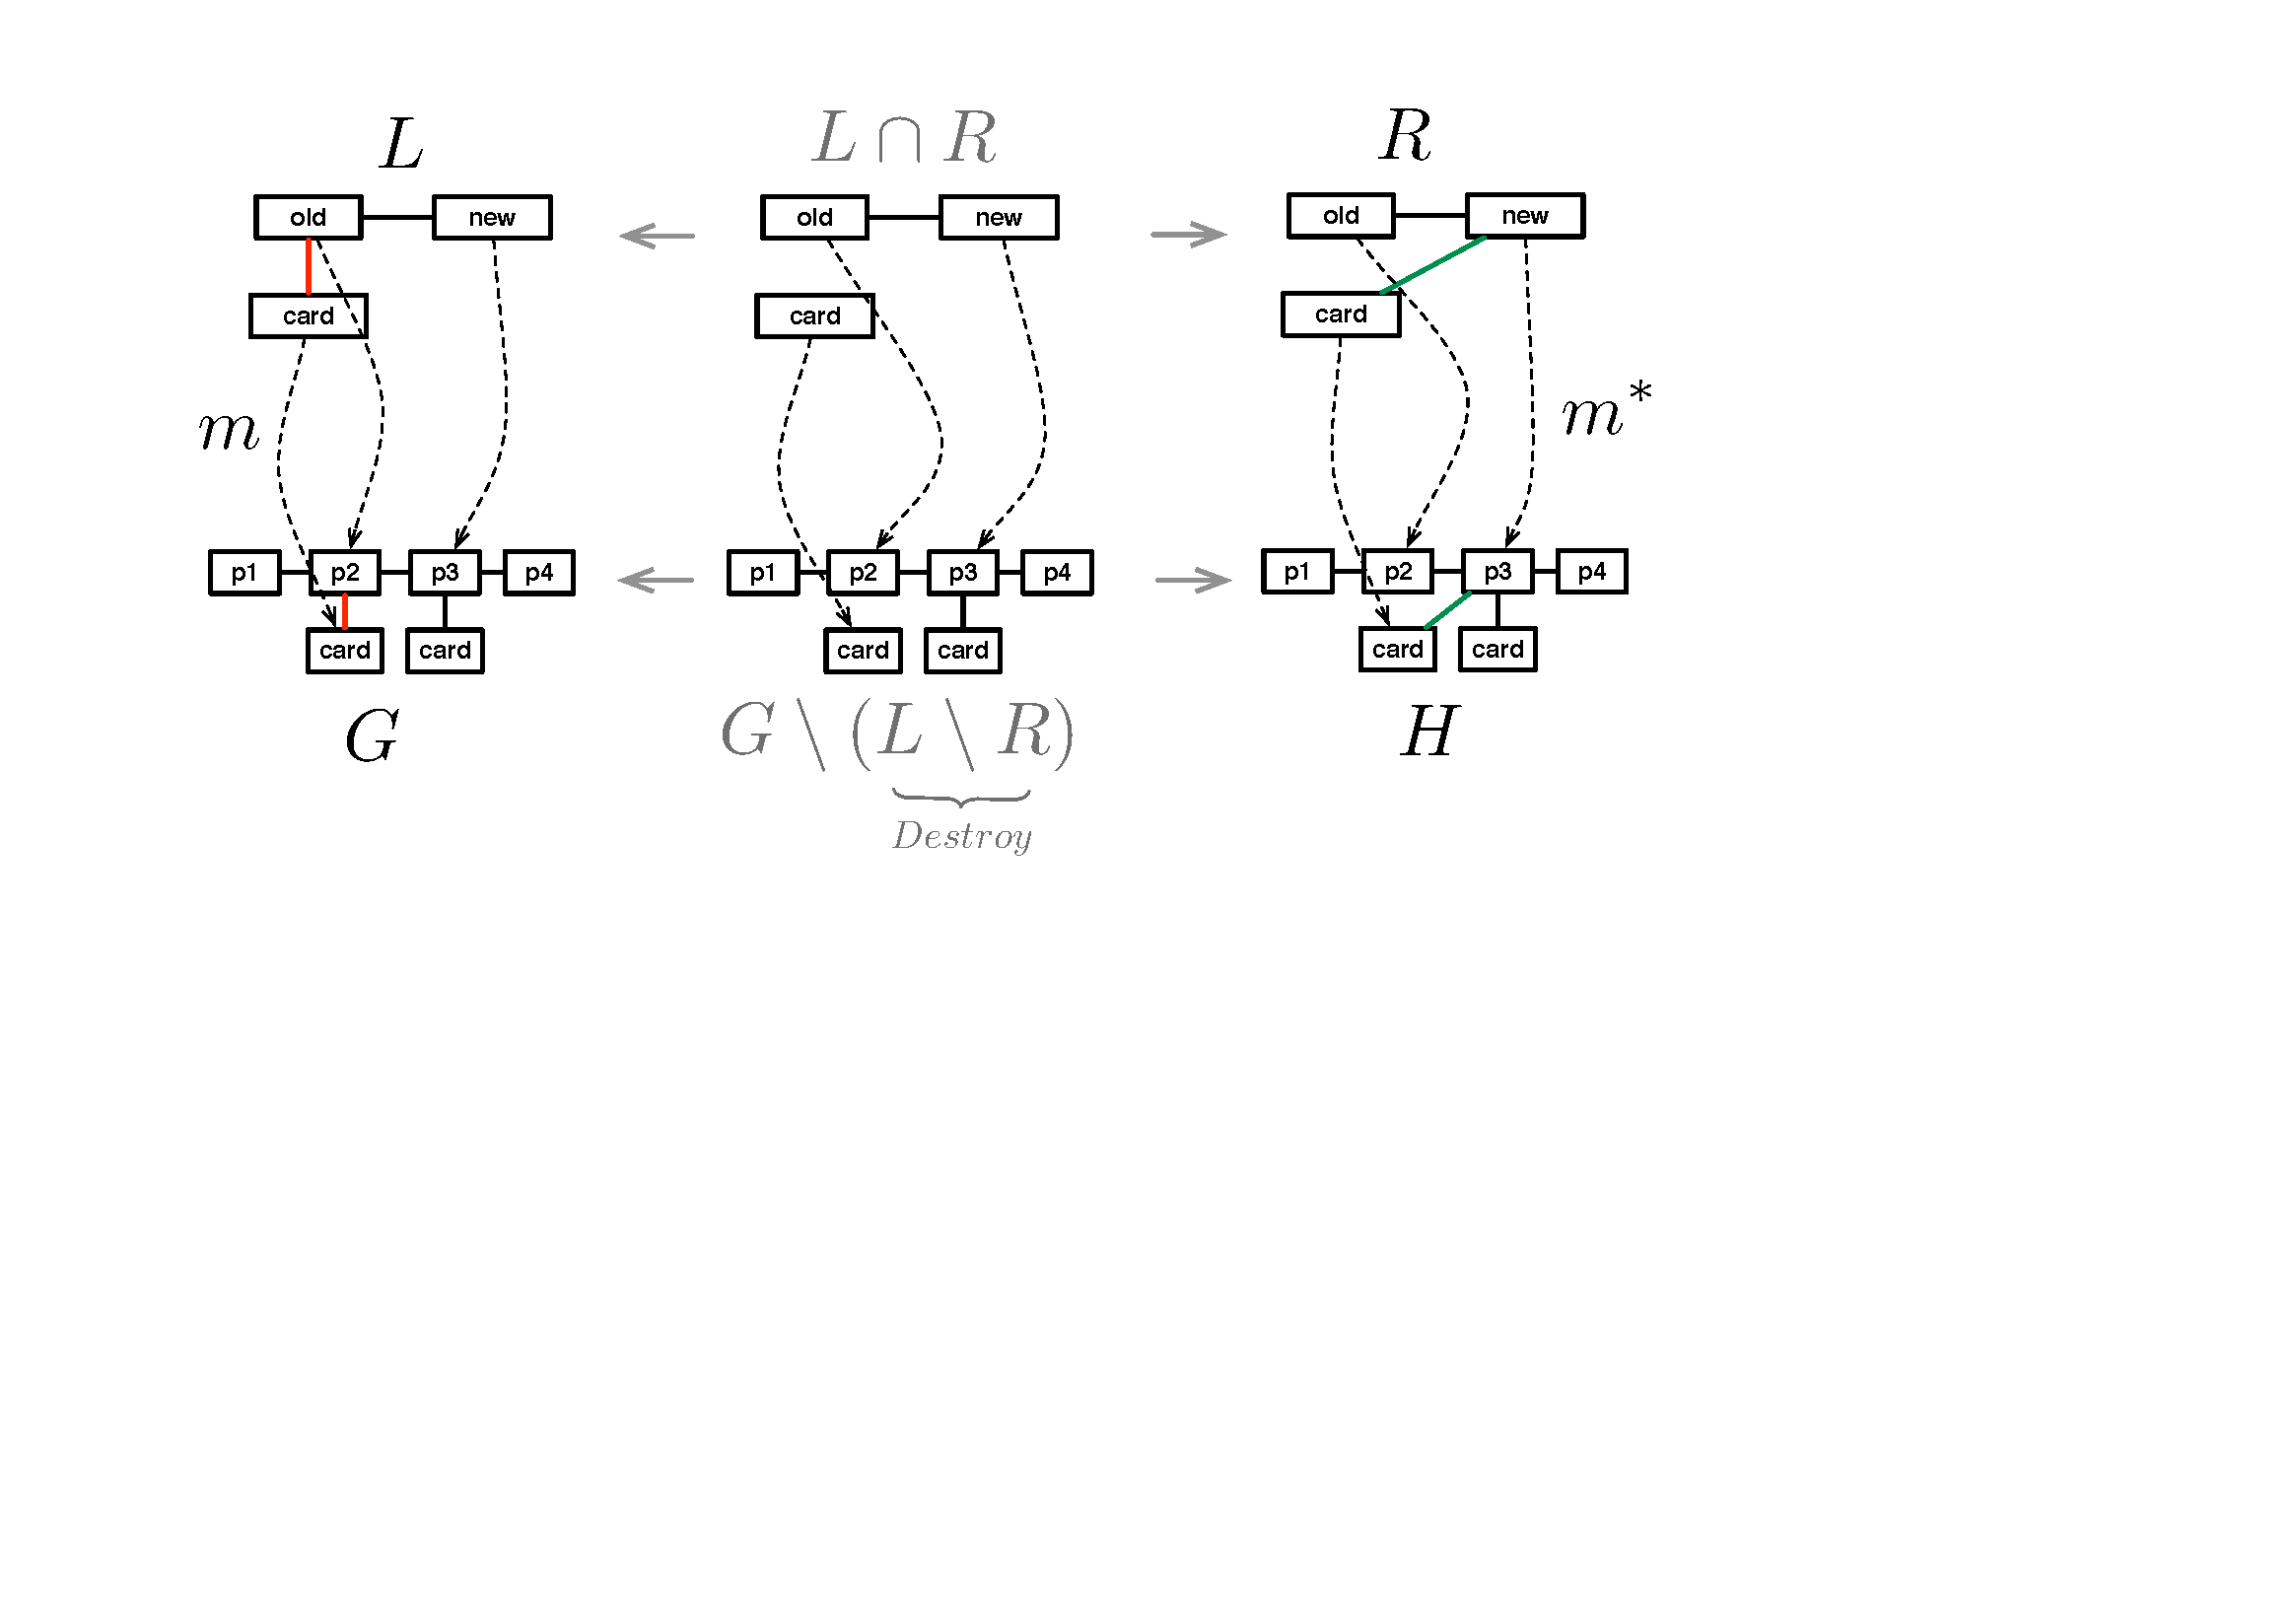
\includegraphics[width=\textwidth]{pics/rule_app_example}
  \caption[]{Applying $moveCard$ to a memory box.}
  \label{fig:rule_app_example}
\end{center}
\end{figure}

\clearpage 

One last thing before we continue with our memory box; individual rules still
have to be applied in a suitable sequence to realise complex model
transformations that consist of many steps.  This is realised with simplified
activity diagrams, where a single activity node is a pattern as discussed above,
and activity edges join nodes to form a control flow.   This can be viewed as
two layers:  an imperative layer to define the top-level control flow via
activity diagrams (if-else statements, loops etc), and a pattern layer
consisting of a story pattern in each activity node that specifies, via a graph
transformation rule, how the model is to be manipulated in that step.         

Enough theory! Grab your mouse and let's get cracking with SDMs\ldots
\subsection{Removing cards from a partition}

In EA, open the main diagram (double-click in the project browser) and carefully do the following: (1) \emph{Click once} on \texttt{Partition} to select it, then (2) \emph{click once} on the method \texttt{removeCard} to choose it (Fig.~\ref{fig:sdm_start}). 
\note{Create an SDM} 
(3) \emph{Double-click} on the chosen method to indicate that you want to implement it.

\begin{figure}[htp]
\begin{center}
  \includegraphics[width=0.4\textwidth]{pics/sdmBilder/removeCard/sdm01RAW}
  \caption{Double-click a method to implement it.}  
  \label{fig:sdm_start}
\end{center}
\end{figure}
 
If you did everything right, a new \emph{activity diagram} should be created \note{Activity Diagram} with a cute little \emph{start node} labelled with the signature of the method \note{Start Node} as depicted in Fig.~\ref{fig:sdm_skeleton}.  Inspect your project browser and note that an \texttt{SDM\_Container} has been created for the method \texttt{removeCard} to contain the diagram.  
If you're at any time unhappy with an SDM\footnote{As you might have already noticed, we use ``SDM'' interchangeably to mean our graph transformation language or a concrete transformation (a story model) used to implement a method and consisting of an activity diagram and a pattern in each story node.  
This will all be explained in detail.}, you can always delete the appropriate container in the project browser and start from scratch, following the steps described previously to create a skeleton for a new SDM.  
Also note the new \note{SDM Toolbox} toolbox \texttt{SDM} that has been automatically opened up for the diagram and placed to the left above the common toolbox. 

\begin{figure}[htp]
\begin{center}
  \includegraphics[width=0.9\textwidth]{pics/sdmBilder/removeCard/sdm02RAW}
  \caption{Generated SDM diagram and start node.}  
  \label{fig:sdm_skeleton}
\end{center}
\end{figure}

Now it's time to complete our very first activity. 
Choose the start node, and note the small black arrow that appears (Fig.~\ref{fig:sdm_quicklink}).  

\clearpage
Similar to quick linking which we learnt when creating our metamodel, a further fundamental gesture in EA is \emph{Quick
\note{Quick Create} 
Create}. 
To quick create an element, pull the arrow and click on an empty spot in the diagram where the new element is to be created.  
This is basically quick linking to a non-existent element if you wish.

\begin{figure}[htp]
\begin{center}
  \includegraphics[width=0.5\textwidth]{pics/sdmBilder/removeCard/sdm03RAW}
  \caption{Quick link in SDM diagram to create new activity node.}  
  \label{fig:sdm_quicklink}
\end{center}
\end{figure}

EA notices that there is nothing to quick link to and pops up a small context-sensitive dialogue, not for creating a link as in the case of quick linking, but for creating an element that can be connected to the indicated source element. 

As indicated in Fig.~\ref{fig:sdm_new_activity_node} choose \texttt{Append StoryNode} to create an \emph{activity node}.  
We
\note{Activity}
\note{Activity Node}
\note{Activity Edge}
shall refer to the whole activity diagram simply as an \emph{activity} that always starts with a start node, terminates with a \emph{stop node} and consists of activity nodes connected via \emph{activity edges}.  
If you quick created correctly, you should now have a start node, an activity node called \texttt{ActivityNode 1} and an edge connecting the start node and the activity node.

\begin{figure}[htp]
\begin{center}
  \includegraphics[width=0.8\textwidth]{pics/sdmBilder/removeCard/sdm04RAW}
  \caption{Create new activity node.}  
  \label{fig:sdm_new_activity_node}
\end{center}
\end{figure}

Complete the activity by quick creating a stop node as depicted in Fig.~\ref{fig:sdm_stop_node}.

\begin{figure}[htp]
\begin{center}
  \includegraphics[width=\textwidth]{pics/sdmBilder/removeCard/sdm05RAW}
  \caption{Complete activity with a stop node.}  
  \label{fig:sdm_stop_node}
\end{center}
\end{figure}

If you did that right as well you should now have a complete activity that models the procedural \emph{control flow} of our method.  
The semantics of our activities is pretty straightforward -- the control flow starts in the start node and flows along edges and connected activity nodes till it terminates in a stop node.  
The complete activity is depicted in Fig.~\ref{fig:sdm_complete_control_flow_simple} now with the activity node connected via an activity edge to the newly created stop node.

\label{story-pattern}

Integrated as an atomic step in this overall control flow, a single graph
\note{Story Pattern}
transformation step can be embedded in some activity nodes as a \emph{story pattern}.  
These story patterns are declarative transformation rules as introduced in Sec.~\ref{sec:sdm_intro}.  
As not all activity nodes can contain story
\note{Story Node}
patterns (e.g. start and stop nodes), those that can are called \emph{story nodes}. 

\begin{figure}[htp]
\begin{center}
  \includegraphics[width=\textwidth]{pics/sdmBilder/removeCard/sdm06RAW.pdf}
  \caption{Control flow modelled as a simple activity diagram.}  
  \label{fig:sdm_complete_control_flow_simple}
\end{center}
\end{figure}

To create a story pattern, double click the story node \texttt{ActivityNode 1} in Fig.~\ref{fig:sdm_complete_control_flow_simple} to prompt the dialogue depicted in Fig.~\ref{fig:story_pattern}.  
Enter \texttt{remove\-Card\-From\-Partition} as the name of the story node, check \texttt{Create this Object} and click \texttt{OK}.

\begin{figure}[htpb]
\begin{center} 
  \includegraphics[width=0.45\textwidth]{pics/sdmBilder/removeCard/sdm07RAW.png}
  \caption{Start modelling story pattern in activity node.}  
  \label{fig:story_pattern}
\end{center}
\end{figure}

The activity node should now have a single \emph{object variable} \texttt{this}
\note{Object Variable}
(Fig.~\ref{fig:tool_box}). 
Object variables are, as the word ``variable'' indicates, place holders for actual objects in a model.  
During \emph{pattern matching},
\note{Pattern Matching}
actual objects in the  current model are assigned to the object variables in the pattern according to  the indicated type of the object variable and other conditions\footnote{We shall learn what conditions can be specified in a
few pages.}. 
In our case, the current story pattern consists of only one object variable, which is assigned (per convention) to \texttt{this} in Java (the object whose method is invoked).

\begin{figure}[htp]
\begin{center}
  \includegraphics[width=0.8\textwidth]{pics/sdmBilder/removeCard/sdm09RAW}
  \caption{Add a new object variable from the tool-box.}  
  \label{fig:tool_box}
\end{center}
\end{figure}

To create an object variable that can be assigned to other objects, choose \texttt{SDM ObjectVariable} from the toolbox as indicated in
Fig.~\ref{fig:tool_box} and click \emph{in the} activity node \texttt{removeCardFromPartition} (Fig.~\ref{fig:object_variable_properties}). 


\begin{figure}[htp]
\begin{center}
  \includegraphics[width=0.8\textwidth]{pics/sdmBilder/removeCard/sdm10RAW}
  \caption{Specify properties of the added object variable.}  
  \label{fig:object_variable_properties}
\end{center}
\end{figure}

In the dialogue that pops up, choose \texttt{toBeRemoved} as the name of the object variable and \texttt{Card} as its type using the corresponding drop-down menus. 
Because \texttt{toBeRemoved} is a parameter of the method, it is offered as a possible name in the drop-down menu and can be directly chosen to prevent annoying mistakes due to typing the name of the parameter wrongly.

In the dialogue, note the option \texttt{Bound} that must be set.
For the pattern matcher, bound object variables do not need to be assigned as they already have a fixed value from the context of the method.  
We have already seen two cases  for bound object variables: the assignment to \texttt{this} (the current  partition who owns the method), and assignments to parameters of the 
\note{Binding State}
method that  are specified when invoking the method.  
Please note that the assignment or \emph{binding} is in both cases implicit and via the \emph{name} of the bound object variable. 

\begin{figure}[htp]
\begin{center}
  \includegraphics[width=0.55\textwidth]{pics/sdmBilder/removeCard/sdm11RAW}
  \caption{Create a link variable.}   
  \label{fig:link_variable}
\end{center}
\end{figure}

Models consist not only of objects but also of \emph{links}.  
To match links one can thus create \emph{link variables} in story patterns that act as place 
\note{Link Variable}
holders for links in a model.  
To create a link variable between the current partition, whose \texttt{removeCard} method is invoked, and the card to be removed, which is passed in as a parameter of the method, choose the object variable \texttt{this} and quick link it to the object variable \texttt{toBeRemoved}.  
In the quick link dialogue choose \texttt{Create LinkVariable} (Fig.~\ref{fig:link_variable}).

In the property dialogue that pops up, choose the offered link type (according to the metamodel, there is only one possible link type between a partition and a 
\note{Binding Operator}
card), and set the \emph{Binding Operator} to \texttt{Destroy} (Fig.~\ref{fig:link_variable_properties}). 
Every object or link variable's binding operator can be set to one of \texttt{Check Only, Create, Destroy}.

\begin{figure}[htp] 
\begin{center} 
 \includegraphics[width=0.6\textwidth]{pics/sdmBilder/removeCard/sdm12RAW.png}
  \caption{Specify properties for created link variable.}  
  \label{fig:link_variable_properties}
\end{center}
\end{figure}



For a rule $r: (L, R)$, as discussed in Sec.~\ref{sec:sdm_intro}, this marks the variable as belonging to the set of elements to be retained ($L\cap R$), the set of elements to be newly created ($R\setminus L$), or the set of elements to be deleted ($L\setminus R$).
 
According to the signature of the method \texttt{removeCard}, we should return the card that has been deleted.  
Although this might strike you as slightly odd, considering that we already passed in this exact card as an argument, it still makes sense as it allows for chaining method calls: \begin{quote}\texttt{aPartition.removeCard(aCard).invert()}\end{quote}
In any case, a return value for an SDM can be specified in the stop node.
\note{Return Values}
As depicted in Fig.~\ref{fig:stop_node_return_value}, double-click the stop node to prompt the \texttt{Edit StopNode} dialogue.
\note{Expressions}
In the \texttt{Expression} field, choose \texttt{ParameterExpression}, and \texttt{toBeRemoved} as the parameter.  
In many different dialogues, we employ a simple context-sensitive expression language for specifying required values.  
We have intentionally avoided creating a full-blown sub-language and limit expressions to a few simple types\footnote{We also do not support nesting expressions}.  
The philosophy here is to keep things simple and concentrate on what SDMs are good for -- expressing structural change.  
Our approach is to provide a clear and type-safe interface to a general purpose language (in our case Java) and support a simple \emph{fallback} as soon as things get low-level and difficult to express as a pattern.  

\begin{figure}[htp]
\begin{center}
  \includegraphics[width=0.95\textwidth]{pics/sdmBilder/removeCard/sdm14RAW.png}
  \caption{Adding a return value to the stop node.}  
  \label{fig:stop_node_return_value}
\end{center}
\end{figure}

The alternative approach would be to support arbitrary expressions, for example, in a script language like JavaScript or in an appropriate DSL\footnote{A DSL is a Domain Specific Language: a language designed for a specific task which is usually simpler than a general purpose language like Java and more suitable for the exact task.} designed for this purpose. 
In a few pages we'll learn the other expression types
\note{Parameter Expression}
we support and how to use them, for the moment, a \emph{Parameter Expression} is used to refer to one of the parameters of the current method, which is exactly what we needed and have used for our \texttt{removeCard} SDM.
If you've done everything right, your complete SDM should now look like Fig.~\ref{fig:sdm_complete_control_flow} with the return value indicated below the stop node.

Let's take a step back and review briefly what we have specified:  if \texttt{p.remove\-Card(c)} is invoked for a partition \texttt{p} with a card \texttt{c} as argument, the specified pattern will \emph{match} if the card is contained in the partition.
After determining a match for all variables, the link between the partition and the card is deleted, effectively ``removing'' the card from the partition.  

If the card is \emph{not} contained in the partition, the pattern won't match and nothing happens. 
In both cases the card that was passed in is simply returned.

\begin{figure}[htbp]
\begin{center}
  \includegraphics[width=0.7\textwidth]{pics/sdmBilder/removeCard/sdm15}
  \caption{Complete SDM for \texttt{Partition::removeCard}.}  
  \label{fig:sdm_complete_control_flow}
\end{center}
\end{figure}

Congratulations!  You have specified your very first SDM.  
Don't forget to export and generate code in your Eclipse workspace. 
Inspect the generated implementation for the method\footnote{The generated method is in \texttt{/Learning\-Box\-Language/\-gen/\-Learning\-Box\-Language/\-impl/\-Partition\-Impl.java/\-remove\-Card}} and see if you can get a feel for what the generated code does. 
Notice all the null checks that are generated automatically -- only a very conscientious (and probably slightly paranoid) programmer would program so defensively!

If you're unable to export or generate code successfully, compare your SDM carefully with Fig.~\ref{fig:sdm_complete_control_flow} and make sure you haven't forgotten anything.

In the following sections, we shall explore further features of SDM that allow for really expressive and powerful patterns.

\subsection{Checking a card}

The next method we shall model with SDMs is probably the most important: a user decides to try a card in the learning box and looks at the question on the card (\texttt{Card.face}), makes a guess and \emph{checks} to see if the guess was correct by comparing with the answer on the back of the card (\texttt{Card.back}).
If the guess was correct the card can be \emph{promoted} by moving it to the \emph{next} partition, if it was wrong the card is \emph{penalized} by moving it to the \emph{previous} partition.

As you're almost an SDM wizard already, try, using concepts we have already learnt, to create the control flow for \texttt{Partition::check} as depicted in Fig.~\ref{fig:sdm_check_start}.

\begin{figure}[htbp]
\begin{center}
  \includegraphics[width=\textwidth]{pics/sdmBilder/check/sdm16RAW.pdf}
  \caption{Activity diagram for \texttt{Partition::check}.}
  \label{fig:sdm_check_start}
\end{center}
\end{figure}

To check if the guess was correct, create an object variable that is bound to
the argument \texttt{card}, representing the card the user has picked from the
learning box.  Remember that this binding is implicitly specified by choosing the
name of the argument as the name of the object variable
(Fig.~\ref{fig:sdm_check_addCard}).

\begin{figure}[htbp]
\begin{center}
  \includegraphics[width=\textwidth]{pics/sdmBilder/check/sdm17RAW}
  \caption{Add the card to be checked.}
  \label{fig:sdm_check_addCard}
\end{center}
\end{figure}

Now that we have the card to be checked, we need to compare the user's guess to
\note{Attribute Constraint}
the actual answer on the back of the card.  To do this we need to specify an
\emph{Attribute Constraint}.  An attribute constraint is a
non-structural condition that must be satisfied for a story pattern to match,
and can be specified by choosing the \texttt{Attribute Constraint} tab as
depicted in Fig.~\ref{fig:sdm_check_att_constraint}.  In this dialogue, choose
the attribute to be used in formulating the constraint (\texttt{back}) and the
type of \texttt{Expression} used to express the constraint.  As we shall compare
the back of the card with the user's guess, passed in as a parameter, we need a
\texttt{ParameterExpression} to refer to this value.  In the previous section,
we already used parameter expressions to specify the return value in a stop
node.  Now choose the parameter (\texttt{guessed}) and the type of
constraint or \emph{operation} to be executed -- in this case an equality check
(\texttt{==}). Press the button labelled \texttt{Add} and admire your first
attribute constraint (Fig.~\ref{fig:sdm_check_att_constraint})!

\begin{figure}[htbp]
\begin{center}
  \includegraphics[width=0.8\textwidth]{pics/sdmBilder/check/sdm18RAW}
  \caption{Add an attribute constraint with a parameter expression.}
  \label{fig:sdm_check_att_constraint}
\end{center}
\end{figure}

Let's get back to the control flow for a bit.  We need to specify that the card
is to be penalised if the guess was wrong (the story node
\texttt{Check\-If\-Guess\-Is\-Correct} did not match) and to be promoted if it
was correct (a match could be found, i.e., all constraints/conditions both
\note{Edge Guards}
structural and non-structural could be fulfilled).  Such an if/else construct is
specified in SDMs via \emph{Edge Guards}.  To add a guard to the edge leading
from \texttt{Check\-If\-Guess\-Is\-Correct} to \texttt{penalize\-Card}, double
\note{Guard Type}
click the edge and choose the \emph{Guard Type} in the dialogue
(Fig.~\ref{fig:sdm_check_guard}).  

Choose \texttt{Failure}, repeat the process
for the edge leading to \texttt{promoteCard} and choose \texttt{Success}.

\begin{figure}[htbp]
\begin{center}
  \includegraphics[width=0.75\textwidth]{pics/sdmBilder/check/sdm19}
  \caption{Add a transition with a guard.}
  \label{fig:sdm_check_guard}
\end{center}
\end{figure}


The next feature of our tool we shall learn is a means of coping with large
patterns.  It might be nice to visualise \emph{small} story patterns directly in
their story nodes, but for large patterns or complex surrounding control flow,
such diagrams would get very cumbersome and unwieldy pretty quickly.  This is
indeed a popular argument against visual languages and it might already have
crossed your mind (``this is cute, but it'll \emph{never} scale!'').  With the
right tools and concepts however, even huge diagrams can be mastered.  We
\note{Extracting Patterns}
support \emph{extracting} story patterns to their own extra diagrams and
recommend this for most cases (unless the pattern is really concise and
only contains about 2-3 object variables).

\begin{figure}[htbp]
\begin{center}
  \includegraphics[width=0.75\textwidth]{pics/sdmBilder/check/sdm21}
  \caption{Extract a story pattern for more space and a better overview.}
  \label{fig:sdm_check_extract_storypattern}
\end{center}
\end{figure}

To extract an empty or already
partially modelled story pattern, just double-click the corresponding story node
(\texttt{promoteCard}) and choose \texttt{Extract Story Pattern}
(Fig.~\ref{fig:sdm_check_extract_storypattern}). Note the new diagram that is
immediately opened and created in the project browser
(Fig.~\ref{fig:sdm_new_sub_diagram}).

\begin{figure}[htbp]
\begin{center}
  \includegraphics[width=0.75\textwidth]{pics/sdmBilder/check/sdm_new_storypattern_diagram.png}
  \caption{A new sub diagram is created automatically.}
  \label{fig:sdm_new_sub_diagram}
\end{center}
\end{figure}

\begin{figure}[htbp]
\begin{center}
  \includegraphics[width=\textwidth]{pics/sdmBilder/check/sdm22RAW}
  \caption{Add an object variable per drag and drop.}
  \label{fig:sdm_check_bound_card}
\end{center}
\end{figure}

Yet another EA gesture is good old \emph{Drag and Drop} from the project
\note{Drag \& Drop}
browser\footnote{Remember the other two gestures we have learnt:  Quick Link
and Quick Create.}, which we use as an alternative to the SDM toolbox.
To create an object variable, simply drag and drop the class
\texttt{Card} from the project browser and into the extracted story
pattern diagram (Fig.~\ref{fig:sdm_check_bound_card}).  A dialogue should pop-up
asking if you want to (1) create a simple link (referring to \texttt{Card} as a
class) or (2) create an Object (as an instance of \texttt{Card}), or (3), if you
want to create a subclass.  In our case we want to create an object(variable)
and so (2) is nearest in meaning.  As this \texttt{Paste Element} dialogue is a
bit annoying, EA  allows you to choose a default for \emph{all} drag and drop
gestures.  Go ahead and check \texttt{All Drag and Drop} so that option (2) is
used next time as the default.  Furthermore, you should also check
\texttt{Only show this dialog when Ctrl+Mouse drag is used}, so that the
default is used \emph{without} popping up this dialogue for confirmation. Don't worry,
if you ever need options (1) and (3), for example when metamodelling, you  just
need to hold \texttt{Ctrl} when dragging to invoke the dialogue and change  the
settings to suit the current modelling activity.

After creating the object, you will be asked to set the object variable properties. Set its \texttt{Name} to ''card'' and its \texttt{Binding State} to ''Bound'' (Fig.~\ref{fig:sdm_new_card_properties}).

\begin{figure}[htbp]
\begin{center}
  \includegraphics[width=0.5\textwidth]{pics/sdmBilder/check/sdm23.png}
  \caption{Object variable properties of the new card.}
  \label{fig:sdm_new_card_properties}
\end{center}
\end{figure}

The main advantage of drag and drop is that the \texttt{Object Variable
Pro\-per\-ties} dialogue that now pops-up should have the type of the object
variable pre-configured. Choosing the type in the project browser and dragging it in
is for most people a more natural gesture than choosing the type from a long
drop-down menu and can really be a great time saver for large
metamodels\footnote{Drag and drop is also possible in embedded story patterns
(still visualised in their story nodes).  You must ensure however, that the
object variable is \emph{completely} contained inside the story node and does
not stick out over any edge}.

Let's move on with the current pattern. Remember that we want to promote the
card.  As a first step drag and drop two further object variables for
\texttt{this} (the current partition) and the next partition according to
(Fig.~\ref{fig:sdm_check_complete_sp}).  An important point to note here is
that \texttt{this} and \texttt{card} are visually differentiated from
\texttt{nextPartition} by their bold border lines. This is how we differentiate
\emph{bound} \note{Bound vs. Unbound} variables (\texttt{this, card}) from
\emph{unbound} or \emph{free} variables like \texttt{nextPartition}.  We already know that matches for bound variables are completely determined by the current
context (argument of the method, current ``this" object).  Matches for unbound
variables on the other hand, have to be determined by the pattern matcher.  Such
matches are ``found'' by navigating and searching in the current model for
possible matches that satisfy all specified constraints (e.g. type of the
variable, links connecting it to other variables and attribute constraints).

\begin{figure}[htbp]
\begin{center}
  \includegraphics[width=0.8\textwidth]{pics/sdmBilder/check/sdm25.pdf}
  \caption{All object variables for story pattern \texttt{promoteCard}.}
  \label{fig:sdm_check_complete_sp}
\end{center}
\end{figure}

In our case, the next partition has to be determined, by navigating from
\texttt{this} via the \texttt{next} link in the metamodel.  Make sure the bound
checkbox for \texttt{nextPartition} is left empty and quick link from
\texttt{this} to \texttt{nextPartition}, or vice-versa, to create a
\texttt{next} link variable as indicated in
Fig.~\ref{fig:sdm_check_link_variable}.

\begin{figure}[htbp]
\begin{center}
  \includegraphics[width=0.85\textwidth]{pics/sdmBilder/check/sdm26}
  \caption{Create a link variable.}
  \label{fig:sdm_check_link_variable}
\end{center}
\end{figure}

If you've done everything right, your story pattern should now closely resemble
Fig.~\ref{fig:sdm_check_complete_activity_node}.  Take a step back and reflect
on what the pattern expresses.

\begin{figure}[htbp]
\begin{center}
  \includegraphics[width=0.8\textwidth]{pics/sdmBilder/check/sdm30}
  \caption{Complete story pattern for activity node \texttt{promoteCard}.}
  \label{fig:sdm_check_complete_activity_node}
\end{center}
\end{figure}

Now repeat the process for the story node \texttt{penalizeCard}: extract the
story pattern, and create all variables as depicted in
Fig.~\ref{fig:sdm_check_complete_penalize}.  This pattern is quite similar to
\texttt{promoteCard} but moves the card from \texttt{this} to \texttt{previous}
instead of \texttt{next}.  Just like before, \texttt{previousPartition} is
unbound and must be determined by navigating from \texttt{this} along the link
\texttt{previous}.

\begin{figure}[htbp]
\begin{center}
  \includegraphics[width=0.8\textwidth]{pics/sdmBilder/check/sdm38}
  \caption{Story pattern for activity node \texttt{penalizeCard}.}
  \label{fig:sdm_check_complete_penalize}
\end{center}
\end{figure}

To complete our SDM, we need to signalise, as a return value, if the guess was
correct or not (and consequently if the card was promoted or penalised).  To do
\note{Literal Expression}
this, double-click the stop node after \texttt{promoteCard} and choose
\texttt{LiteralExpression} as the type of expression
(Fig.~\ref{fig:sdm_check_literal_exp}).

\begin{figure}[htbp]
\begin{center}
  \includegraphics[width=0.6\textwidth]{pics/sdmBilder/check/sdm39}
  \caption{Add a return value with a literal expression.}
  \label{fig:sdm_check_literal_exp}
\end{center}
\end{figure}

\emph{Literal expressions} can be used
to specify arbitrary text.  This should actually be used only for
\emph{literals} like 42, ``foo'' or \texttt{true} but can of course be (mis)used
for formulating any (Java) expression that will simply be transferred
``literally'' into the  generated code. This is obviously sort of
dirty\footnote{It defeats, for example, any attempt to guarantee type safety.}
and should be avoided if possible.

\begin{figure}[htbp]
\begin{center}
  \includegraphics[width=0.8\textwidth]{pics/sdmBilder/check/sdm40}
  \caption{Complete SDM for \texttt{Partition::check}.}
  \label{fig:sdm_check_finish}
\end{center}
\end{figure}

Type in \texttt{true} as the value of the expression
(Fig.~\ref{fig:sdm_check_literal_exp}) and complete the SDM by returning
\texttt{false} after penalising a card.  Please ensure that your SDM (the
control flow) closely resembles Fig.~\ref{fig:sdm_check_finish}.  As always,
export the project, generate code and inspect the implementation for
\texttt{check}.  We strongly recommend that you even write a simple JUnit test
(take a look at our simple test case in Sec.~\ref{sec:junit} for inspiration)
to take your brand new SDM for a test-spin.

\subsection{Emptying a partition of all its cards}
\label{sec:empty}

The next SDM we shall specify should \emph{empty} a partition of all its cards,
deleting the cards in the process.  To do this we obviously need a construct for
repeating the action for all cards in the partition.  In SDM, this is
\note{For Each}
accomplished via a \emph{For Each} story node.  A for each story node performs
the specified actions for \emph{every} match of its story pattern.  To create a
for each story node, create the initial diagram and start node for the method
\texttt{Partition::empty} and quick create an activity node choosing
\texttt{ForEach} as its type (Fig.~\ref{fig:sdm_foreach}).

\begin{figure}[htp]
\begin{center}
  \includegraphics[width=0.5\textwidth]{pics/sdmBilder/empty/sdm42RAW}
  \caption{A for each loop in SDM.}  
  \label{fig:sdm_foreach}
\end{center}
\end{figure}

A for each story node is visualised as a double node to indicate the
potential repetition (Fig.~\ref{fig:sdm_end}). Complete the story pattern as
indicated in Fig.~\ref{fig:sdm_end}.  Please note that the \texttt{card} that is
deleted in each match is unbound and both the \texttt{card} and link to
\texttt{this} are set to \texttt{destroy}.  Even more important, note that the
guard that terminates the for each story node has an \texttt{[end]} guard. 
Indeed, a for each story node \emph{must} have an end activity edge which is
taken when all matches for the story pattern have been handled.

There are two interesting points to note: First of all, how would the pattern be
interpreted if the story node where a normal story node and not a for each?
\note{Non-Determinism}  
Well, the pattern would specify that \emph{a} card should
be matched and deleted from the current partition.  Note that the \emph{exact}
card is not specified and indeed the actual choice of the card is
\emph{non-deterministic} or random.  This is a common property of graph
transformations and pattern matching and is something that takes some getting
used to. In general, there are no guarantees concerning the choice and order of
valid matches.

\begin{figure}[htp]
\begin{center}
  \includegraphics[width=0.6\textwidth]{pics/sdmBilder/empty/sdm47}
  \caption{Complete story pattern with \texttt{[end]} guard.}  
  \label{fig:sdm_end}
\end{center}
\end{figure}

The second point is if we need to destroy the link between \texttt{this} and
\texttt{card}.  Would the pattern be interpreted differently if we just
destroyed \texttt{card} and left the link?  The answer is no, the pattern would
yield the same result, regardless of if the link is explicitly destroyed or not.
This is because the transformation engine we use\footnote{CodeGen2 which is
part of Fujaba \url{http://www.fujaba.de/}} ensures that there are never any
\note{Dangling Edges}
\emph{dangling edges} in a model.  As deleting only \texttt{card} would result
in a ``dangling edge'' attached to \texttt{this}, the link is deleted as well.
Explicitly destroying the link or not is therefore a matter of taste, but \ldots
why not be as explicit as possible?

\subsection{Turning a card around} 

The next SDM \emph{inverts} a card by swapping its back and face values.  This
therefore ``turns the card around'' in the learning box, which makes sense when
learning, for example, a new language.  You're no longer an SDM beginner so try
to model the SDM depicted in Fig.~\ref{fig:sdm_invert}.

\begin{figure}[htp]
\begin{center}
  \includegraphics[width=0.7\textwidth]{pics/sdmBilder/invert/sdm54}
  \caption{Swap back and face of the card.}  
  \label{fig:sdm_invert}
\end{center}
\end{figure}

Something new here is that we use \emph{assignments} to set the attributes of
\note{Assignments}
\texttt{temp} in \texttt{Initialize temp} and to swap the attributes of
\texttt{this} in \texttt{Swap variables}.  An assignment is an attribute
constraint with \texttt{:=} as operation.  Although it might be slightly
confusing to refer to an assignment as a constraint, if you think a while about
it \emph{everything} can be viewed as a constraint that can be fulfilled via
different strategies.  In this case, an assignment is fulfilled not by searching
\note{Assertion}
for a match, as in the case of an assertion (\texttt{==, >, <, \ldots}), but by
\emph{performing} the assignment.  Similarly, non-context elements (set to
create or destroy) can be viewed as structural constraints that are fulfilled by
creating or destroying the corresponding element.  A constraint is therefore
a unifying concept similar to ``everything is an object'' from OO and
``everything is a model'' from metamodelling and has the usual advantages.  If
\note{Unification} 
you're interested in why unification is considered cool check out \cite{BEZ05}.

A last point before we move on to the next SDM.  Did you notice that
\texttt{temp} is bound in the story pattern of \texttt{Swap variables}?  This is
a new case for bound variables that we haven't treated yet.  Till now we have
seen object variables that can be (1) bound to an argument of the method that is
set when the method is invoked, or (2) bound to the current object
\texttt{this} whose method is invoked.  In both cases, the object to be matched
is completely determined by the context of the method and does not need to be
determined by the pattern matcher.  

Setting \texttt{temp} as bound in
\texttt{Swap variables} is a third case in which an object variable is bound
to the value already determined in a \emph{previous activity node}.  This means
that in our case, the object variable \texttt{temp} in \texttt{Swap variables}
is to be bound to the value determined for the unbound object variable
\texttt{temp} in \texttt{Initialize temp}.  This way, you can always refer to
previous matches for object variables in the preceding control flow.  Please
note that the reference or mapping is again implicit via the same \emph{name} of
the object variable.  As in the case of arguments of the method, the editor
provides rudimentary support via a drop-down menu which can be used
to choose the name of an object variable and avoid possible mistakes when
typing by hand.

\subsection{Growing the box by adding a new partition}
\label{sec:sdm_grow}	
	
In this SDM, we shall specify how our learning box is built up and how the
contained partitions are connected.  This controls how cards move back and
forward in the box.  Although very different behaviour can be implemented, we
shall implement the classical rules as depicted in
Fig.~\ref{fig:membox_illustration}.

Start off by creating the simple control flow and story pattern depicted in
Fig.~\ref{fig:sdm_grow_1}.  This matches the box (\texttt{this}), and
\emph{any} two partitions in the box.
	
\begin{figure}[htbp]
\begin{center}
  \includegraphics[width=\textwidth]{pics/sdmBilder/grow/sdm57.pdf}
  \caption{Context elements for SDM.}  
  \label{fig:sdm_grow_1}
\end{center}
\end{figure}

As already indicated by the chosen names of the object variables
\texttt{first\-Partition} and \texttt{last\-Partition\-In\-Box}, we actually
want the pattern matcher to determine the first and the last partition in the box.
But how do we specify this?  As explained in section \ref{sec:empty}, the
current story pattern will simply determine two partitions
non-deterministically.  

SDMs provide a declarative means of identifying the first and last
partition via \emph{Negative Application Conditions}, also simply
referred to as \mbox{NACs}\footnote{Pronounced $\backslash 'nak \backslash$}.
A \mbox{NAC} is a negative element that should \emph{not} be present in a valid
\note{\mbox{NACs}}
match.  In the theory of algebraic graph transformations \cite{EEPT06},
\mbox{NACs} can be complex graphs that are much more general and powerful.  In
our implementation\footnote{To be more precise CodeGen2 from Fujaba.}, however,
we only support single negative elements (object or link variables).

To create an appropriate \mbox{NAC} that constrains the possible matches for
\texttt{lastPartitionInBox} to exactly the last partition in the box, create a
new object variable \texttt{nextPartition} of type \texttt{Partition} and set
\note{Binding Semantics}
its \emph{Binding Semantics} to \texttt{negative} (Fig.~\ref{fig:sdm_grow_2}).  
The object variable should be visualised as being cancelled or struck out.
 
\begin{figure}[htbp]
\begin{center}
  \includegraphics[width=0.9\textwidth]{pics/sdmBilder/grow/sdm58RAW}
  \caption{Adding a negative element.}  
  \label{fig:sdm_grow_2}
\end{center}
\end{figure}
 
Now quick link \texttt{nextPartition} to \texttt{lastPartitionInBox} and choose
the link type carefully, so that \texttt{nextPartition} plays the role of
\texttt{next} with respect to \texttt{lastPartitionInBox}.  Now complete the
story pattern so that it closely resembles Fig.~\ref{fig:sdm_grow_3}.  The
\mbox{NACs} can be interpreted as follows:  The first/last partition in the box
is \emph{a} partition in the box that has no previous/next partition.  The
valid matches are made unique and thus deterministic by construction, i.e., if
you \emph{grow} the box via this method, there will always be exactly one first
and one last partition.  

\begin{figure}[htbp]
\begin{center}
  \includegraphics[width=\textwidth]{pics/sdmBilder/grow/sdm65}
  \caption{Determining the first and last partition with NACs.}  
  \label{fig:sdm_grow_3}
\end{center}
\end{figure}
 
Note how the newly created partition
\texttt{newPartition} is hung into the box (it becomes the next partition of the
current last partition and has as its previous partition the first partition
in the box) according to the arrows in Fig.~\ref{fig:membox_illustration}.
  
All that is missing to complete our SDM is an assignment to set the size of the
new partition.  We already know that an assignment is an attribute
constraint with \texttt{:=} as operator so go ahead and invoke the corresponding
dialogue.  As the new size must be calculated depending on the rest of the
partitions in the box (partitions usually get bigger) we call a helper function
\note{MethodCallExpression}
via a \emph{MethodCallExpression}.  A MethodCallExpression is used to invoke a
method that is defined in a class in the current EA project.  Enter the values
in Fig.~\ref{fig:sdm_grow_4} choosing the argument \texttt{helper} as target and
\texttt{determineNextSize} as the method to be invoked.  Parameters can be
specified by just choosing the appropriate parameter declaration between
guillemets (e.g. \texttt{<Box box>}) via the drop-down menu and typing in the
value (this is basically a literal expression). So, be sure that \texttt{<Box box>} is selected
from the drop down menu and replace its text with \texttt{this}. Don't forget to
press the \texttt{Save} button for every parameter and \texttt{Add} 
+ \texttt{OK} to confirm and close the dialogue.
 
\begin{figure}[htbp]
\begin{center}
  \includegraphics[width=0.5\textwidth]{pics/sdmBilder/grow/sdm66}
  \caption{Invoking a method via a \texttt{MethodCallExpression}.}  
  \label{fig:sdm_grow_4}
\end{center}
\end{figure}

If you've done everything right, your SDM should now closely resemble
Fig.~\ref{fig:sdm_grow_5}.  As usual, try to export, generate code, inspect the
method implementation and write a JUnit test.  This time around you also have to
implement the helper method \texttt{determineNextSize} directly in the
generated code
(\texttt{gen/\-LearningBoxLanguage/\-facade/\-impl/\-LearningBoxUtilImpl}).
Don't forget to add \texttt{@generated NOT} to the Java doc comment of the
method so the code generator preserves your code in future runs.
When testing (which you will \emph{of course} do right?), note that you can only grow a ``minimal'' box that has at least a first and last partition, i.e., a box with no partitions at all cannot be grown using our specified SDM. 

\begin{figure}[htbp]
\begin{center}
  \includegraphics[width=\textwidth]{pics/sdmBilder/grow/sdm67}
  \caption{Complete SDM for \texttt{Box::grow}.}  
  \label{fig:sdm_grow_5}
\end{center}
\end{figure}

\subsection{A string representation for our memory box}

With the next SDM, we shall create a string representation for a complete memory
box.  To accomplish this, we have to iterate through all cards in all partitions
which involves an inner loop nested in an outer loop.  SDMs support arbitrary nesting
of For Each story nodes via special guards.  In Sec.~\ref{sec:empty} we already
used the \texttt{[end]} edge guard to terminate a loop and, as depicted in
\note{[each time]}
Fig.~\ref{fig:sdm_tostring_1}, an \texttt{[each time]} guard is used to indicate
control flow that is \emph{nested} in the For Each story node and is executed
for each match.

Go ahead and create the SDM for \texttt{Box::toString} till it closely resembles
Fig.~\ref{fig:sdm_tostring_1}.  The first For Each \texttt{ForAllPartitions}
matches all partitions and each partition is used \texttt{[each time]} in
\texttt{ForAllCards} to match all cards.  Note that \texttt{partition} in
\texttt{ForAllCards} is bound  and thus refers to the assigned value determined
in \texttt{ForAllParitions}.  When all cards have been matched,
\texttt{ForAllCards} terminates or \texttt{[end]}s and returns to the outer loop
\texttt{ForAllPartitions}.

\begin{figure}[htbp]
\begin{center}
  \includegraphics[width=\textwidth]{pics/sdmBilder/toString/sdm72}
  \caption{Control flow with nested loops.}  
  \label{fig:sdm_tostring_1}
\end{center}
\end{figure}

To actually do something sensible with each card, double-click the empty
activity node that is taken each time a card is matched and invoke the \texttt{Edit
ActivityNode} dialogue.  Now choose \texttt{printCard} as
the name, and \texttt{StatementNode} as the type of the activity node
(Fig.~\ref{fig:sdm_tostring_2}).
\note{Statement Nodes}
A statement node is used to invoke a method from a class in any package in the
current EA project via a MethodCallExpression.  This way, the method invocation
is represented as an activity node and is guaranteed to be executed at this
point in the control flow. 

\begin{figure}[htbp]
\begin{center}
  \includegraphics[width=0.7\textwidth]{pics/sdmBilder/toString/sdm73}
  \caption{Invoking a method in a \texttt{StatementNode}.}  
  \label{fig:sdm_tostring_2}
\end{center}
\end{figure}

As we have already used a MethodCallExpression in an attribute constraint
(Sec.~\ref{sec:sdm_grow}), go ahead and click the \texttt{Method Call
Expression} tab and invoke the \texttt{printCard} operation on \texttt{helper}
with the current \texttt{card} as its argument (Fig.~\ref{fig:sdm_tostring_3}).

Statement nodes should be used to interact with methods that are
implemented by hand and provide a means of invoking libraries and arbitrary Java
code from SDMs.  Please note that we do not differentiate at this point between
methods that are implemented via an SDM or by hand and thus, statement nodes can
\note{Recursion}
of course be used to invoke other SDMs via a MethodCallExpression.  Most
importantly, this enables \emph{recursion} as the current SDM can be invoked on
\texttt{this} with appropriate new arguments.  

A final point to note is that the
return value of the method is ignored -- statement nodes are therefore best used
for void methods that either have appropriate side effects (e.g. manipulate
their arguments).  We shall learn in a few pages how to invoke methods with
non-primitive return values (if a method returns a primitive then it can be
invoked in an attribute constraint as in Sec.~\ref{sec:sdm_grow}).

\begin{figure}[htbp]
\begin{center}
  \includegraphics[width=0.35\textwidth]{pics/sdmBilder/toString/sdm74}
  \caption{Specify a \texttt{MethodCallExpression} in the
  \texttt{StatementNode}.}
  \label{fig:sdm_tostring_3}
\end{center}
\end{figure}

To complete the SDM, retrieve the final string representation from the helper by
returning via a MethodCallExpression in the stop node
(Fig.~\ref{fig:sdm_tostring_4}). 

\begin{figure}[htbp]
\begin{center}
  \includegraphics[width=0.576\textwidth]{pics/sdmBilder/toString/sdm75}
  \caption{Using a \texttt{MethodCallExpression} as a return value.}  
  \label{fig:sdm_tostring_4}
\end{center}
\end{figure}

Take some time to compare and reflect on the complete SDM as depicted in
Fig.~\ref{fig:sdm_tostring_5}.  The idea was to abstract from the actual text
representation of the box and model the necessary traversal of the data
structure.  The helper methods \texttt{printCard} and
\texttt{getStringRep} could, for example, build up a string buffer and return
the final string representation respectively.  While modelling this SDM, we have
seen that for each story nodes can be nested, and have learnt two new uses of
MethodCallExpressions that provide a type safe\footnote{Apart from the literal
expressions used for specifying argument values.} means of invoking methods from
SDMs.

\begin{figure}[htbp]
\begin{center}
  \includegraphics[width=0.7\textwidth]{pics/sdmBilder/toString/sdm76}
  \caption{The complete SDM for \texttt{Box::toString}.}  
  \label{fig:sdm_tostring_5}
\end{center}
\end{figure}

As usual, export, generate code, inspect the generated method implementations
and write some tests.  Just like in Sec.~\ref{sec:sdm_grow}, don't forget to
implement the helper methods!

\subsection{Handling ``fast'' cards}
	
For very simple cards (e.g. words in different language that are so similar), it
might be a bit annoying to have to answer these cards again and again in every
partition.  Such \emph{fast} cards can be marked as such and handled
differently:  If a fast card is gotten right once it should be immediately moved
to the last partition in the box.  This way the card is learnt once and is
tested only once more before it is finally removed from the box.

To introduce fast cards to our learning box go to the metamodel and create a new
eclass \texttt{FastCard}.  Quick link to \texttt{Card} and choose
\texttt{Inheritance} from the quick link context menu
(Fig.~\ref{fig:sdm_fastcard_1}). 

\begin{figure}[htp]
\begin{center}
  \includegraphics[width=0.4\textwidth]{pics/sdmBilder/bindings/fastcard}
  \caption{Fast cards are a special kind of card.}  
  \label{fig:sdm_fastcard_1}
\end{center}
\end{figure}

Now go to the SDM \texttt{check} in \texttt{Partition} and extend the control
flow as depicted in Fig.~\ref{fig:sdm_fastcard_2}. 
 
Add new story nodes
\texttt{is fast card?} and \texttt{promote fast card} and drag and drop a bound
object variable \texttt{fastcard} \emph{of type} \texttt{FastCard} into \texttt{is fast card?}.  

\begin{figure}[htbp]
\begin{center}
  \includegraphics[width=0.75\textwidth]{pics/sdmBilder/bindings/fastcard_controlflow.pdf}
  \caption{Extend check to handle fast cards.}  
  \label{fig:sdm_fastcard_2}
\end{center}
\end{figure}

What we need to do now is decide, based on the dynamic
type\footnote{In a statically typed language like Java, every object has a
static type (determined at compile time) and a dynamic type (that can only be
determined at runtime).} of \texttt{card} if we must handle a fast card or not.
This can be expressed in SDMs via \emph{BindingExpressions} or just
\emph{Bindings}.  A binding can be specified for a \emph{bound} object variable
\note{Bindings}
and represents the final case where an object variable can be marked as being
bound.  

To refresh your memory, we have already learnt that a bound object
variable is either (1) assigned to \texttt{this}, (2) a parameter of the method,
or (3) a value determined in a preceding activity node.  Bindings represent a
fourth possibility of giving a manual binding for an object variable. 

To create a binding for \texttt{fastcard}, choose the \texttt{Binding} tab in
the \texttt{Object Variable Properties} dialogue
(Fig.~\ref{fig:sdm_fastcard_3}). 

\begin{figure}[htbp]
\begin{center}
  \includegraphics[width=0.6\textwidth]{pics/sdmBilder/bindings/fastcard_bindingexp.png}
  \caption{Create a binding for \texttt{fastcard}.}  
  \label{fig:sdm_fastcard_3}
\end{center}
\end{figure}

As usual all our expression types can be used for the \texttt{Binding
Expression}.  Since we already know all the types let's consider what each type
would mean in this context: 
\begin{description}
  \item[MethodCallExpression:]~\\ This would allow invoking a method and binding
  its return value to the object variable.  This is how non-primitive return
  values of methods can be used safely in SDMs.
  \item[ParameterExpression:]~\\ This could be used to bind the object variable
  to a parameter of the method.  If the object variable is of a different type
  than the parameter (e.g. a subtype) this represents basically a successful
  typecast if the pattern matches.
  \item[LiteralExpression:]~\\ As usual this can be anything and is literally
  copied with a surrounding typecast into the generated code.  Using
  LiteralExpressions too often is usually a sign for not thinking in a
  \emph{pattern oriented} manner and is considered a \emph{bad smell}.
  \item[ObjectVariableExpression:]~\\ This can be used to refer to other object
  variables in preceding story nodes.  Just like for ParameterExpressions, this
  represents a simple typecast if the types of the \texttt{target} and the
  object variable with the binding are different.
\end{description}

In our case, we could use a ParameterExpression or an ObjectVariableExpression as
\texttt{card} is indeed a parameter \emph{and} has already been used in
\texttt{checkIfGuessIsCorrect}.  As we haven't used ObjectVariableExpressions
before lets try it out!  Choose \texttt{ObjectVariableExpression} as the type of
the binding expression and \texttt{card} from the drop-down menu as the target. 
If you've done everything right, the binding should be visualised concisely as
in Fig.~\ref{fig:sdm_fastcard_4}.
 
\begin{figure}[htbp]
\begin{center}
  \includegraphics[width=0.3\textwidth]{pics/sdmBilder/bindings/visual_bindingexp}
  \caption{Visualisation for binding expression.}  
  \label{fig:sdm_fastcard_4}
\end{center}
\end{figure}

To complete the SDM, extract the story pattern of \texttt{promote fast card} and
specify the pattern according to Fig.~\ref{fig:sdm_fastcard_5}.  The fast card
is transferred from the current partition \texttt{this}, to the last partition
in the box, which is identified with an appropriate \mbox{NAC} (already used in
Sec.~\ref{sec:sdm_grow}). 

\begin{figure}[htbp]
\begin{center}
  \includegraphics[width=\textwidth]{pics/sdmBilder/bindings/promoteFastCard}
  \caption{Story pattern for handling fast cards.}  
  \label{fig:sdm_fastcard_5}
\end{center}
\end{figure}

Export, generate code and inspect the new implementation for \texttt{check}. 
Can you find the generated type casts for \texttt{fastcard}?  Don't forget to
write a few tests and see if fast cards are handled correctly!


 
\chapter{Conclusion} 

Wow!  If you've really worked through everything till now (and performed all those extra tests), then you can consider yourself a \emph{bona fide} eMoflon wizard.
Get yourself a nice cool beer -- you've really earned it!

We hope you enjoyed the trip, if you have any suggestions, questions, feedback or corrections (all those screenshots get outdated so quickly!), please contact us \url{contact@moflon.org}.

Our tool \emph{eMoflon} is constantly evolving so don't forget to check out what's new at \url{www.moflon.org}
 

% Start appendix
\begin{appendix}
% adjust page numbering 
\pagenumbering{roman}
\setcounter{page}{\value{romanpages}}
\addtocounter{page}{1} 
\let\originalclearpage=\clearpage
\def\clearpage{\relax}
\renewcommand*{\bibname}{}
\chapter{References}\vskip-4cm
\bibliographystyle{plain}  
\bibliography{references} 
\newpage

\newcommand{\nocontentsline}[3]{}
\newcommand{\tocless}[2]{\bgroup\let\addcontentsline=\nocontentsline#1{#2}\egroup}

\tocless\chapter{GNU GENERAL PUBLIC LICENSE}
\label{chap:gpl}
\scriptsize
\begin{floatingfigure}[l]{2.7cm}
	\includegraphics[width=2.7cm]{pics/gplv3.png}	
\end{floatingfigure}

                    GNU GENERAL PUBLIC LICENSE
                       Version 3, 29 June 2007

 Copyright (C) 2007 Free Software Foundation, Inc. \url{http://fsf.org/}
 Everyone is permitted to copy and distribute verbatim copies
 of this license document, but changing it is not allowed.

Preamble

  The GNU General Public License is a free, copyleft license for
software and other kinds of works.

  The licenses for most software and other practical works are designed
to take away your freedom to share and change the works.  By contrast,
the GNU General Public License is intended to guarantee your freedom to
share and change all versions of a program--to make sure it remains free
software for all its users.  We, the Free Software Foundation, use the
GNU General Public License for most of our software; it applies also to
any other work released this way by its authors.  You can apply it to
your programs, too.

  When we speak of free software, we are referring to freedom, not
price.  Our General Public Licenses are designed to make sure that you
have the freedom to distribute copies of free software (and charge for
them if you wish), that you receive source code or can get it if you
want it, that you can change the software or use pieces of it in new
free programs, and that you know you can do these things.

  To protect your rights, we need to prevent others from denying you
these rights or asking you to surrender the rights.  Therefore, you have
certain responsibilities if you distribute copies of the software, or if
you modify it: responsibilities to respect the freedom of others.

  For example, if you distribute copies of such a program, whether
gratis or for a fee, you must pass on to the recipients the same
freedoms that you received.  You must make sure that they, too, receive
or can get the source code.  And you must show them these terms so they
know their rights.

  Developers that use the GNU GPL protect your rights with two steps:
(1) assert copyright on the software, and (2) offer you this License
giving you legal permission to copy, distribute and/or modify it.

  For the developers' and authors' protection, the GPL clearly explains
that there is no warranty for this free software.  For both users' and
authors' sake, the GPL requires that modified versions be marked as
changed, so that their problems will not be attributed erroneously to
authors of previous versions.

  Some devices are designed to deny users access to install or run
modified versions of the software inside them, although the manufacturer
can do so.  This is fundamentally incompatible with the aim of
protecting users' freedom to change the software.  The systematic
pattern of such abuse occurs in the area of products for individuals to
use, which is precisely where it is most unacceptable.  Therefore, we
have designed this version of the GPL to prohibit the practice for those
products.  If such problems arise substantially in other domains, we
stand ready to extend this provision to those domains in future versions
of the GPL, as needed to protect the freedom of users.

  Finally, every program is threatened constantly by software patents.
States should not allow patents to restrict development and use of
software on general-purpose computers, but in those that do, we wish to
avoid the special danger that patents applied to a free program could
make it effectively proprietary.  To prevent this, the GPL assures that
patents cannot be used to render the program non-free.

  The precise terms and conditions for copying, distribution and
modification follow.

                       TERMS AND CONDITIONS

  0. Definitions.

  ``This License'' refers to version 3 of the GNU General Public License.

  ``Copyright'' also means copyright-like laws that apply to other kinds of
works, such as semiconductor masks.

  ``The Program'' refers to any copyrightable work licensed under this
License.  Each licensee is addressed as ``you''.  ``Licensees'' and
``recipients'' may be individuals or organizations.

  To ``modify'' a work means to copy from or adapt all or part of the work
in a fashion requiring copyright permission, other than the making of an
exact copy.  The resulting work is called a ``modified version'' of the
earlier work or a work ``based on'' the earlier work.

  A ``covered work'' means either the unmodified Program or a work based
on the Program.

  To ``propagate'' a work means to do anything with it that, without
permission, would make you directly or secondarily liable for
infringement under applicable copyright law, except executing it on a
computer or modifying a private copy.  Propagation includes copying,
distribution (with or without modification), making available to the
public, and in some countries other activities as well.

  To ``convey'' a work means any kind of propagation that enables other
parties to make or receive copies.  Mere interaction with a user through
a computer network, with no transfer of a copy, is not conveying.

  An interactive user interface displays ``Appropriate Legal Notices''
to the extent that it includes a convenient and prominently visible
feature that (1) displays an appropriate copyright notice, and (2)
tells the user that there is no warranty for the work (except to the
extent that warranties are provided), that licensees may convey the
work under this License, and how to view a copy of this License.  If
the interface presents a list of user commands or options, such as a
menu, a prominent item in the list meets this criterion.

  1. Source Code.

  The ``source code'' for a work means the preferred form of the work
for making modifications to it.  ``Object code'' means any non-source
form of a work.

  A ``Standard Interface'' means an interface that either is an official
standard defined by a recognized standards body, or, in the case of
interfaces specified for a particular programming language, one that
is widely used among developers working in that language.

  The ``System Libraries'' of an executable work include anything, other
than the work as a whole, that (a) is included in the normal form of
packaging a Major Component, but which is not part of that Major
Component, and (b) serves only to enable use of the work with that
Major Component, or to implement a Standard Interface for which an
implementation is available to the public in source code form.  A
``Major Component'', in this context, means a major essential component
(kernel, window system, and so on) of the specific operating system
(if any) on which the executable work runs, or a compiler used to
produce the work, or an object code interpreter used to run it.

  The ``Corresponding Source'' for a work in object code form means all
the source code needed to generate, install, and (for an executable
work) run the object code and to modify the work, including scripts to
control those activities.  However, it does not include the work's
System Libraries, or general-purpose tools or generally available free
programs which are used unmodified in performing those activities but
which are not part of the work.  For example, Corresponding Source
includes interface definition files associated with source files for
the work, and the source code for shared libraries and dynamically
linked subprograms that the work is specifically designed to require,
such as by intimate data communication or control flow between those
subprograms and other parts of the work.

  The Corresponding Source need not include anything that users
can regenerate automatically from other parts of the Corresponding
Source.

  The Corresponding Source for a work in source code form is that
same work.

  2. Basic Permissions.

  All rights granted under this License are granted for the term of
copyright on the Program, and are irrevocable provided the stated
conditions are met.  This License explicitly affirms your unlimited
permission to run the unmodified Program.  The output from running a
covered work is covered by this License only if the output, given its
content, constitutes a covered work.  This License acknowledges your
rights of fair use or other equivalent, as provided by copyright law.

  You may make, run and propagate covered works that you do not
convey, without conditions so long as your license otherwise remains
in force.  You may convey covered works to others for the sole purpose
of having them make modifications exclusively for you, or provide you
with facilities for running those works, provided that you comply with
the terms of this License in conveying all material for which you do
not control copyright.  Those thus making or running the covered works
for you must do so exclusively on your behalf, under your direction
and control, on terms that prohibit them from making any copies of
your copyrighted material outside their relationship with you.

  Conveying under any other circumstances is permitted solely under
the conditions stated below.  Sublicensing is not allowed; section 10
makes it unnecessary.

  3. Protecting Users' Legal Rights From Anti-Circumvention Law.

  No covered work shall be deemed part of an effective technological
measure under any applicable law fulfilling obligations under article
11 of the WIPO copyright treaty adopted on 20 December 1996, or
similar laws prohibiting or restricting circumvention of such
measures.

  When you convey a covered work, you waive any legal power to forbid
circumvention of technological measures to the extent such circumvention
is effected by exercising rights under this License with respect to
the covered work, and you disclaim any intention to limit operation or
modification of the work as a means of enforcing, against the work's
users, your or third parties' legal rights to forbid circumvention of
technological measures.

  4. Conveying Verbatim Copies.

  You may convey verbatim copies of the Program's source code as you
receive it, in any medium, provided that you conspicuously and
appropriately publish on each copy an appropriate copyright notice;
keep intact all notices stating that this License and any
non-permissive terms added in accord with section 7 apply to the code;
keep intact all notices of the absence of any warranty; and give all
recipients a copy of this License along with the Program.

  You may charge any price or no price for each copy that you convey,
and you may offer support or warranty protection for a fee.

  5. Conveying Modified Source Versions.

  You may convey a work based on the Program, or the modifications to
produce it from the Program, in the form of source code under the
terms of section 4, provided that you also meet all of these conditions:

    a) The work must carry prominent notices stating that you modified
    it, and giving a relevant date.

    b) The work must carry prominent notices stating that it is
    released under this License and any conditions added under section
    7.  This requirement modifies the requirement in section 4 to
    ``keep intact all notices''.

    c) You must license the entire work, as a whole, under this
    License to anyone who comes into possession of a copy.  This
    License will therefore apply, along with any applicable section 7
    additional terms, to the whole of the work, and all its parts,
    regardless of how they are packaged.  This License gives no
    permission to license the work in any other way, but it does not
    invalidate such permission if you have separately received it.

    d) If the work has interactive user interfaces, each must display
    Appropriate Legal Notices; however, if the Program has interactive
    interfaces that do not display Appropriate Legal Notices, your
    work need not make them do so.

  A compilation of a covered work with other separate and independent
works, which are not by their nature extensions of the covered work,
and which are not combined with it such as to form a larger program,
in or on a volume of a storage or distribution medium, is called an
``aggregate'' if the compilation and its resulting copyright are not
used to limit the access or legal rights of the compilation's users
beyond what the individual works permit.  Inclusion of a covered work
in an aggregate does not cause this License to apply to the other
parts of the aggregate.

  6. Conveying Non-Source Forms.

  You may convey a covered work in object code form under the terms
of sections 4 and 5, provided that you also convey the
machine-readable Corresponding Source under the terms of this License,
in one of these ways:

    a) Convey the object code in, or embodied in, a physical product
    (including a physical distribution medium), accompanied by the
    Corresponding Source fixed on a durable physical medium
    customarily used for software interchange.

    b) Convey the object code in, or embodied in, a physical product
    (including a physical distribution medium), accompanied by a
    written offer, valid for at least three years and valid for as
    long as you offer spare parts or customer support for that product
    model, to give anyone who possesses the object code either (1) a
    copy of the Corresponding Source for all the software in the
    product that is covered by this License, on a durable physical
    medium customarily used for software interchange, for a price no
    more than your reasonable cost of physically performing this
    conveying of source, or (2) access to copy the
    Corresponding Source from a network server at no charge.

    c) Convey individual copies of the object code with a copy of the
    written offer to provide the Corresponding Source.  This
    alternative is allowed only occasionally and noncommercially, and
    only if you received the object code with such an offer, in accord
    with subsection 6b.

    d) Convey the object code by offering access from a designated
    place (gratis or for a charge), and offer equivalent access to the
    Corresponding Source in the same way through the same place at no
    further charge.  You need not require recipients to copy the
    Corresponding Source along with the object code.  If the place to
    copy the object code is a network server, the Corresponding Source
    may be on a different server (operated by you or a third party)
    that supports equivalent copying facilities, provided you maintain
    clear directions next to the object code saying where to find the
    Corresponding Source.  Regardless of what server hosts the
    Corresponding Source, you remain obligated to ensure that it is
    available for as long as needed to satisfy these requirements.

    e) Convey the object code using peer-to-peer transmission, provided
    you inform other peers where the object code and Corresponding
    Source of the work are being offered to the general public at no
    charge under subsection 6d.

  A separable portion of the object code, whose source code is excluded
from the Corresponding Source as a System Library, need not be
included in conveying the object code work.

  A ``User Product'' is either (1) a ``consumer product'', which means any
tangible personal property which is normally used for personal, family,
or household purposes, or (2) anything designed or sold for incorporation
into a dwelling.  In determining whether a product is a consumer product,
doubtful cases shall be resolved in favor of coverage.  For a particular
product received by a particular user, ``normally used'' refers to a
typical or common use of that class of product, regardless of the status
of the particular user or of the way in which the particular user
actually uses, or expects or is expected to use, the product.  A product
is a consumer product regardless of whether the product has substantial
commercial, industrial or non-consumer uses, unless such uses represent
the only significant mode of use of the product.

  ``Installation Information'' for a User Product means any methods,
procedures, authorization keys, or other information required to install
and execute modified versions of a covered work in that User Product from
a modified version of its Corresponding Source.  The information must
suffice to ensure that the continued functioning of the modified object
code is in no case prevented or interfered with solely because
modification has been made.

  If you convey an object code work under this section in, or with, or
specifically for use in, a User Product, and the conveying occurs as
part of a transaction in which the right of possession and use of the
User Product is transferred to the recipient in perpetuity or for a
fixed term (regardless of how the transaction is characterized), the
Corresponding Source conveyed under this section must be accompanied
by the Installation Information.  But this requirement does not apply
if neither you nor any third party retains the ability to install
modified object code on the User Product (for example, the work has
been installed in ROM).

  The requirement to provide Installation Information does not include a
requirement to continue to provide support service, warranty, or updates
for a work that has been modified or installed by the recipient, or for
the User Product in which it has been modified or installed.  Access to a
network may be denied when the modification itself materially and
adversely affects the operation of the network or violates the rules and
protocols for communication across the network.

  Corresponding Source conveyed, and Installation Information provided,
in accord with this section must be in a format that is publicly
documented (and with an implementation available to the public in
source code form), and must require no special password or key for
unpacking, reading or copying.

  7. Additional Terms.

  ``Additional permissions'' are terms that supplement the terms of this
License by making exceptions from one or more of its conditions.
Additional permissions that are applicable to the entire Program shall
be treated as though they were included in this License, to the extent
that they are valid under applicable law.  If additional permissions
apply only to part of the Program, that part may be used separately
under those permissions, but the entire Program remains governed by
this License without regard to the additional permissions.

  When you convey a copy of a covered work, you may at your option
remove any additional permissions from that copy, or from any part of
it.  (Additional permissions may be written to require their own
removal in certain cases when you modify the work.)  You may place
additional permissions on material, added by you to a covered work,
for which you have or can give appropriate copyright permission.

  Notwithstanding any other provision of this License, for material you
add to a covered work, you may (if authorized by the copyright holders of
that material) supplement the terms of this License with terms:

    a) Disclaiming warranty or limiting liability differently from the
    terms of sections 15 and 16 of this License; or

    b) Requiring preservation of specified reasonable legal notices or
    author attributions in that material or in the Appropriate Legal
    Notices displayed by works containing it; or

    c) Prohibiting misrepresentation of the origin of that material, or
    requiring that modified versions of such material be marked in
    reasonable ways as different from the original version; or

    d) Limiting the use for publicity purposes of names of licensors or
    authors of the material; or

    e) Declining to grant rights under trademark law for use of some
    trade names, trademarks, or service marks; or

    f) Requiring indemnification of licensors and authors of that
    material by anyone who conveys the material (or modified versions of
    it) with contractual assumptions of liability to the recipient, for
    any liability that these contractual assumptions directly impose on
    those licensors and authors.

  All other non-permissive additional terms are considered ``further
restrictions'' within the meaning of section 10.  If the Program as you
received it, or any part of it, contains a notice stating that it is
governed by this License along with a term that is a further
restriction, you may remove that term.  If a license document contains
a further restriction but permits relicensing or conveying under this
License, you may add to a covered work material governed by the terms
of that license document, provided that the further restriction does
not survive such relicensing or conveying.

  If you add terms to a covered work in accord with this section, you
must place, in the relevant source files, a statement of the
additional terms that apply to those files, or a notice indicating
where to find the applicable terms.

  Additional terms, permissive or non-permissive, may be stated in the
form of a separately written license, or stated as exceptions;
the above requirements apply either way.

  8. Termination.

  You may not propagate or modify a covered work except as expressly
provided under this License.  Any attempt otherwise to propagate or
modify it is void, and will automatically terminate your rights under
this License (including any patent licenses granted under the third
paragraph of section 11).

  However, if you cease all violation of this License, then your
license from a particular copyright holder is reinstated (a)
provisionally, unless and until the copyright holder explicitly and
finally terminates your license, and (b) permanently, if the copyright
holder fails to notify you of the violation by some reasonable means
prior to 60 days after the cessation.

  Moreover, your license from a particular copyright holder is
reinstated permanently if the copyright holder notifies you of the
violation by some reasonable means, this is the first time you have
received notice of violation of this License (for any work) from that
copyright holder, and you cure the violation prior to 30 days after
your receipt of the notice.

  Termination of your rights under this section does not terminate the
licenses of parties who have received copies or rights from you under
this License.  If your rights have been terminated and not permanently
reinstated, you do not qualify to receive new licenses for the same
material under section 10.

  9. Acceptance Not Required for Having Copies.

  You are not required to accept this License in order to receive or
run a copy of the Program.  Ancillary propagation of a covered work
occurring solely as a consequence of using peer-to-peer transmission
to receive a copy likewise does not require acceptance.  However,
nothing other than this License grants you permission to propagate or
modify any covered work.  These actions infringe copyright if you do
not accept this License.  Therefore, by modifying or propagating a
covered work, you indicate your acceptance of this License to do so.

  10. Automatic Licensing of Downstream Recipients.

  Each time you convey a covered work, the recipient automatically
receives a license from the original licensors, to run, modify and
propagate that work, subject to this License.  You are not responsible
for enforcing compliance by third parties with this License.

  An ``entity transaction'' is a transaction transferring control of an
organization, or substantially all assets of one, or subdividing an
organization, or merging organizations.  If propagation of a covered
work results from an entity transaction, each party to that
transaction who receives a copy of the work also receives whatever
licenses to the work the party's predecessor in interest had or could
give under the previous paragraph, plus a right to possession of the
Corresponding Source of the work from the predecessor in interest, if
the predecessor has it or can get it with reasonable efforts.

  You may not impose any further restrictions on the exercise of the
rights granted or affirmed under this License.  For example, you may
not impose a license fee, royalty, or other charge for exercise of
rights granted under this License, and you may not initiate litigation
(including a cross-claim or counterclaim in a lawsuit) alleging that
any patent claim is infringed by making, using, selling, offering for
sale, or importing the Program or any portion of it.

  11. Patents.

  A ``contributor'' is a copyright holder who authorizes use under this
License of the Program or a work on which the Program is based.  The
work thus licensed is called the contributor's ``contributor version''.

  A contributor's ``essential patent claims'' are all patent claims
owned or controlled by the contributor, whether already acquired or
hereafter acquired, that would be infringed by some manner, permitted
by this License, of making, using, or selling its contributor version,
but do not include claims that would be infringed only as a
consequence of further modification of the contributor version.  For
purposes of this definition, ``control'' includes the right to grant
patent sublicenses in a manner consistent with the requirements of
this License.

  Each contributor grants you a non-exclusive, worldwide, royalty-free
patent license under the contributor's essential patent claims, to
make, use, sell, offer for sale, import and otherwise run, modify and
propagate the contents of its contributor version.

  In the following three paragraphs, a ``patent license'' is any express
agreement or commitment, however denominated, not to enforce a patent
(such as an express permission to practice a patent or covenant not to
sue for patent infringement).  To ``grant'' such a patent license to a
party means to make such an agreement or commitment not to enforce a
patent against the party.

  If you convey a covered work, knowingly relying on a patent license,
and the Corresponding Source of the work is not available for anyone
to copy, free of charge and under the terms of this License, through a
publicly available network server or other readily accessible means,
then you must either (1) cause the Corresponding Source to be so
available, or (2) arrange to deprive yourself of the benefit of the
patent license for this particular work, or (3) arrange, in a manner
consistent with the requirements of this License, to extend the patent
license to downstream recipients.  ``Knowingly relying'' means you have
actual knowledge that, but for the patent license, your conveying the
covered work in a country, or your recipient's use of the covered work
in a country, would infringe one or more identifiable patents in that
country that you have reason to believe are valid.

  If, pursuant to or in connection with a single transaction or
arrangement, you convey, or propagate by procuring conveyance of, a
covered work, and grant a patent license to some of the parties
receiving the covered work authorizing them to use, propagate, modify
or convey a specific copy of the covered work, then the patent license
you grant is automatically extended to all recipients of the covered
work and works based on it.

  A patent license is ``discriminatory'' if it does not include within
the scope of its coverage, prohibits the exercise of, or is
conditioned on the non-exercise of one or more of the rights that are
specifically granted under this License.  You may not convey a covered
work if you are a party to an arrangement with a third party that is
in the business of distributing software, under which you make payment
to the third party based on the extent of your activity of conveying
the work, and under which the third party grants, to any of the
parties who would receive the covered work from you, a discriminatory
patent license (a) in connection with copies of the covered work
conveyed by you (or copies made from those copies), or (b) primarily
for and in connection with specific products or compilations that
contain the covered work, unless you entered into that arrangement,
or that patent license was granted, prior to 28 March 2007.

  Nothing in this License shall be construed as excluding or limiting
any implied license or other defenses to infringement that may
otherwise be available to you under applicable patent law.

  12. No Surrender of Others' Freedom.

  If conditions are imposed on you (whether by court order, agreement or
otherwise) that contradict the conditions of this License, they do not
excuse you from the conditions of this License.  If you cannot convey a
covered work so as to satisfy simultaneously your obligations under this
License and any other pertinent obligations, then as a consequence you may
not convey it at all.  For example, if you agree to terms that obligate you
to collect a royalty for further conveying from those to whom you convey
the Program, the only way you could satisfy both those terms and this
License would be to refrain entirely from conveying the Program.

  13. Use with the GNU Affero General Public License.

  Notwithstanding any other provision of this License, you have
permission to link or combine any covered work with a work licensed
under version 3 of the GNU Affero General Public License into a single
combined work, and to convey the resulting work.  The terms of this
License will continue to apply to the part which is the covered work,
but the special requirements of the GNU Affero General Public License,
section 13, concerning interaction through a network will apply to the
combination as such.

  14. Revised Versions of this License.

  The Free Software Foundation may publish revised and/or new versions of
the GNU General Public License from time to time.  Such new versions will
be similar in spirit to the present version, but may differ in detail to
address new problems or concerns.

  Each version is given a distinguishing version number.  If the
Program specifies that a certain numbered version of the GNU General
Public License ``or any later version'' applies to it, you have the
option of following the terms and conditions either of that numbered
version or of any later version published by the Free Software
Foundation.  If the Program does not specify a version number of the
GNU General Public License, you may choose any version ever published
by the Free Software Foundation.

  If the Program specifies that a proxy can decide which future
versions of the GNU General Public License can be used, that proxy's
public statement of acceptance of a version permanently authorizes you
to choose that version for the Program.

  Later license versions may give you additional or different
permissions.  However, no additional obligations are imposed on any
author or copyright holder as a result of your choosing to follow a
later version.

  15. Disclaimer of Warranty.

  THERE IS NO WARRANTY FOR THE PROGRAM, TO THE EXTENT PERMITTED BY
APPLICABLE LAW.  EXCEPT WHEN OTHERWISE STATED IN WRITING THE COPYRIGHT
HOLDERS AND/OR OTHER PARTIES PROVIDE THE PROGRAM ``AS IS'' WITHOUT WARRANTY
OF ANY KIND, EITHER EXPRESSED OR IMPLIED, INCLUDING, BUT NOT LIMITED TO,
THE IMPLIED WARRANTIES OF MERCHANTABILITY AND FITNESS FOR A PARTICULAR
PURPOSE.  THE ENTIRE RISK AS TO THE QUALITY AND PERFORMANCE OF THE PROGRAM
IS WITH YOU.  SHOULD THE PROGRAM PROVE DEFECTIVE, YOU ASSUME THE COST OF
ALL NECESSARY SERVICING, REPAIR OR CORRECTION.

  16. Limitation of Liability.

  IN NO EVENT UNLESS REQUIRED BY APPLICABLE LAW OR AGREED TO IN WRITING
WILL ANY COPYRIGHT HOLDER, OR ANY OTHER PARTY WHO MODIFIES AND/OR CONVEYS
THE PROGRAM AS PERMITTED ABOVE, BE LIABLE TO YOU FOR DAMAGES, INCLUDING ANY
GENERAL, SPECIAL, INCIDENTAL OR CONSEQUENTIAL DAMAGES ARISING OUT OF THE
USE OR INABILITY TO USE THE PROGRAM (INCLUDING BUT NOT LIMITED TO LOSS OF
DATA OR DATA BEING RENDERED INACCURATE OR LOSSES SUSTAINED BY YOU OR THIRD
PARTIES OR A FAILURE OF THE PROGRAM TO OPERATE WITH ANY OTHER PROGRAMS),
EVEN IF SUCH HOLDER OR OTHER PARTY HAS BEEN ADVISED OF THE POSSIBILITY OF
SUCH DAMAGES.

  17. Interpretation of Sections 15 and 16.

  If the disclaimer of warranty and limitation of liability provided
above cannot be given local legal effect according to their terms,
reviewing courts shall apply local law that most closely approximates
an absolute waiver of all civil liability in connection with the
Program, unless a warranty or assumption of liability accompanies a
copy of the Program in return for a fee.

                     END OF TERMS AND CONDITIONS

            How to Apply These Terms to Your New Programs

  If you develop a new program, and you want it to be of the greatest
possible use to the public, the best way to achieve this is to make it
free software which everyone can redistribute and change under these terms.

  To do so, attach the following notices to the program.  It is safest
to attach them to the start of each source file to most effectively
state the exclusion of warranty; and each file should have at least
the ``copyright'' line and a pointer to where the full notice is found.

$<$one line to give the program's name and a brief idea of what it
does.$>$ Copyright (C) $<$year$>$  $<$name of author$>$

This program is free software: you can redistribute it and/or
modify it under the terms of the GNU General Public License as published by
    the Free Software Foundation, either version 3 of the License, or
    (at your option) any later version.

This program is distributed in the hope that it will be useful,
    but WITHOUT ANY WARRANTY; without even the implied warranty of
    MERCHANTABILITY or FITNESS FOR A PARTICULAR PURPOSE.  See the
    GNU General Public License for more details.

You should have received a copy of the GNU General Public License
    along with this program.  If not, see \url{http://www.gnu.org/licenses/}.

Also add information on how to contact you by electronic and paper mail.

  If the program does terminal interaction, make it output a short
notice like this when it starts in an interactive mode:

$<$program$>$  Copyright (C) $<$year$>$  $<$name of author$>$
    This program comes with ABSOLUTELY NO WARRANTY; for details type `show w'.
    This is free software, and you are welcome to redistribute it
    under certain conditions; type `show c' for details.

The hypothetical commands `show w' and `show c' should show the appropriate
parts of the General Public License.  Of course, your program's commands
might be different; for a GUI interface, you would use an ``about box''.

You should also get your employer (if you work as a programmer) or school,
if any, to sign a ``copyright disclaimer'' for the program, if necessary.
For more information on this, and how to apply and follow the GNU GPL, see
\url{http://www.gnu.org/licenses/}.


The GNU General Public License does not permit incorporating your program into
proprietary programs.  If your program is a subroutine library, you may
consider it more useful to permit linking proprietary applications with
the library.  If this is what you want to do, use the GNU Lesser General Public
License instead of this License.  But first, please read
\url{http://www.gnu.org/philosophy/why-not-lgpl.html}.




\end{appendix}

\end{document}